% UCL Thesis LaTeX Template
%  See below for info

%%%%%%%%%%%%% Preamble/Setup %%%%%%%%%%%%%%%%%
% This package goes first
\RequirePackage[l2tabu, orthodox]{nag}


% ------ Main document class specification ------
% The draft option here prevents images being inserted,
% Option = phd : )
%\documentclass[12pt,phd,draft,a4paper,oneside]{ucl_thesis}
\documentclass[11pt,phd,a4paper,oneside]{ucl_thesis}
\usepackage{mathptmx}
\usepackage[11pt]{moresize}
\setlength \parskip {1em}

% Package configuration:
% -------- Packages --------

% This package just gives you a quick way to dump in some sample text.
% You can remove it -- it's just here for the examples.
\usepackage{blindtext}

% This package means empty pages (pages with no text) won't get stuff
%  like chapter names at the top of the page. It's mostly cosmetic.
\usepackage{emptypage}

% The graphicx package adds the \includegraphics command,
%  which is your basic command for adding a picture.
\usepackage{graphicx}

% This command is provided by the graphicx package, and 
%  controls the default dpi resolution of images you use.
%  72 is the default, but 300 is more normal, and 600 is
%  as good as you can expect to be able to get on normal paper.
%\pdfimageresolution=300


% The float package improves LaTeX's handling of floats,
%  and also adds the option to *force* LaTeX to put the float
%  HERE, with the [H] option to the float environment.
\usepackage{float}

\usepackage{placeins}

% The amsmath package enhances the various ways of including
%  maths, including adding the align environment for aligned
%  equations.
\usepackage{amsmath}

% Use these two packages together -- they define symbols
%  for e.g. units that you can use in both text and math mode.
\usepackage{gensymb}
\usepackage{textcomp}
% You may also want the units package for making little
%  fractions for unit specifications.
%\usepackage{units}


% The setspace package lets you use 1.5-sized or double line spacing.
\usepackage{setspace}
\setstretch{1.5}

% That just does body text -- if you want to expand *everything*,
%  including footnotes and tables, use this instead:
%\renewcommand{\baselinestretch}{1.5}


% PGFPlots is either a really clunky or really good way to add graphs
%  into your document, depending on your point of view.
% There's waaaaay too much information on using this to cover here,
%  so, you might want to start here:
%   http://pgfplots.sourceforge.net/
%  or here:
%   http://pgfplots.sourceforge.net/pgfplots.pdf
%\usepackage{pgfplots}
%\pgfplotsset{compat=1.3} % <- this fixed axis labels in the version I was using

% PGFPlotsTable can help you make tables a little more easily than
%  usual in LaTeX.
% If you're going to have to paste data in a lot, I'd suggest using it.
%  You might want to start with the manual, here:
%  http://pgfplots.sourceforge.net/pgfplotstable.pdf
%\usepackage{pgfplotstable}

% These settings are also recommended for using with pgfplotstable.
%\pgfplotstableset{
%	% these columns/<colname>/.style={<options>} things define a style
%	% which applies to <colname> only.
%	empty cells with={--}, % replace empty cells with '--'
%	every head row/.style={before row=\toprule,after row=\midrule},
%	every last row/.style={after row=\bottomrule}
%}


% The mhchem package provides chemistry formula typesetting commands
%  e.g. \ce{H2O}
%\usepackage[version=3]{mhchem}

% And the chemfig package gives a weird command for adding Lewis 
%  diagrams, for e.g. organic molecules
%\usepackage{chemfig}

% The linenumbers command from the lineno package adds line numbers
%  alongside your text that can be useful for discussing edits 
%  in drafts.
% Remove or comment out the command for proper versions.
%\usepackage[modulo]{lineno}
% \linenumbers 


% Alternatively, you can use the ifdraft package to let you add
%  commands that will only be used in draft versions
%\usepackage{ifdraft}

% For example, the following adds a watermark if the draft mode is on.
%\ifdraft{
%  \usepackage{draftwatermark}
%  \SetWatermarkText{\shortstack{\textsc{Draft Mode}\\ \strut \\ \strut \\ \strut}}
%  \SetWatermarkScale{0.5}
%  \SetWatermarkAngle{90}
%}


% The multirow package adds the option to make cells span 
%  rows in tables.
\usepackage{multirow}
\usepackage{bm,array}

%%\usepackage{fourier} 
\usepackage{array}
\usepackage{makecell}

\renewcommand\theadalign{bc}
\renewcommand\theadfont{\bfseries}
\renewcommand\theadgape{\Gape[4pt]}
\renewcommand\cellgape{\Gape[4pt]}


% Subfig allows you to create figures within figures, to, for example,
%  make a single figure with 4 individually labeled and referenceable
%  sub-figures.
% It's quite fiddly to use, so check the documentation.
%\usepackage{subfig}

% The natbib package allows book-type citations commonly used in
%  longer works, and less commonly in science articles (IME).
% e.g. (Saucer et al., 1993) rather than [1]
% More details are here: http://merkel.zoneo.net/Latex/natbib.php
%\usepackage{natbib}
\usepackage{url}

% The bibentry package (along with the \nobibliography* command)
%  allows putting full reference lines inline.
%  See: 
%   http://tex.stackexchange.com/questions/2905/how-can-i-list-references-from-bibtex-file-in-line-with-commentary
\usepackage{bibentry} 

% The isorot package allows you to put things sideways 
%  (or indeed, at any angle) on a page.
% This can be useful for wide graphs or other figures.
%\usepackage{isorot}

% The caption package adds more options for caption formatting.
% This set-up makes hanging labels, makes the caption text smaller
%  than the body text, and makes the label bold.
% Highly recommended.
\usepackage[format=hang,font=small,labelfont=bf]{caption}
\usepackage{subcaption}

% If you're getting into defining your own commands, you might want
%  to check out the etoolbox package -- it defines a few commands
%  that can make it easier to make commands robust.
\usepackage{etoolbox}

% For lists
\usepackage{enumitem}
\setlist{nosep}

\usepackage{siunitx}

\DeclareSIUnit\mm{\milli\metre}
\DeclareSIUnit\km{\kilo\metre}


\DeclareSIUnit\micron{\micro\metre}
\DeclareSIUnit\mrad{\milli\rad}
\DeclareSIUnit\gauss{G}
\DeclareSIUnit\eVperc{\eV\per\clight}

\DeclareSIUnit\TeV{\teva\ev}
\DeclareSIUnit\GeV{\giga\ev}
\DeclareSIUnit\MeV{\mega\ev}

\DeclareSIUnit\nanobarn{\nano\barn}
\DeclareSIUnit\picobarn{\pico\barn}
\DeclareSIUnit\femtobarn{\femto\barn}
\DeclareSIUnit\attobarn{\atto\barn}
\DeclareSIUnit\zeptobarn{\zepto\barn}
\DeclareSIUnit\yoctobarn{\yocto\barn}

\DeclareSIUnit\nb{\nano\barn}
\DeclareSIUnit\pb{\pico\barn}
\DeclareSIUnit\fb{\femto\barn}
\DeclareSIUnit\ab{\atto\barn}
\DeclareSIUnit\zb{\zepto\barn}
\DeclareSIUnit\yb{\yocto\barn}

%%%%%% From ATLAS stuff
% +--------------------------------------------------------------------+
% |                                                                    |
% |  Useful things for proton-proton physics                           |
% |                                                                    |
% +--------------------------------------------------------------------+
%
\def\mjj{\ensuremath{m_{jj}}}
\def\pt{\ensuremath{p_{\mathrm{T}}}} % Subscript roman not italic (EE)
\def\pT{\ensuremath{p_{\mathrm{T}}}} % Subscript roman not italic (EE)
\def\et{\ensuremath{E_{\mathrm{T}}}} % Subscript roman not italic (EE)
\def\eT{\ensuremath{E_{\mathrm{T}}}} % Subscript roman not italic (EE)
\def\ET{\ensuremath{E_{\mathrm{T}}}} % Subscript roman not italic (EE)
\def\HT{\ensuremath{H_{\mathrm{T}}}} % Subscript roman not italic (EE)
\def\ptsq{\ensuremath{p^2_{\mathrm{T}}}} % Fixed so it works correctly (EE)

\def\degr{\ensuremath{^\circ}} % Removed mbox - caused problems and not needed (EE)
\def\abseta{\ensuremath{|\eta|}}
\def\Hgg{\ensuremath{H\to\gamma\gamma}}
\def\mh{\ensuremath{m_h}}
\def\mW{\ensuremath{m_W}}
\def\mZ{\ensuremath{m_Z}}
\def\mH{\ensuremath{m_H}}
\def\mA{\ensuremath{m_A}}
\def\MET{\ensuremath{E_{\mathrm{T}}^{\mathrm{miss}}}} % Sub/superscript roman not italic (EE)
\def\met{\ensuremath{E_{\mathrm{T}}^{\mathrm{miss}}}} % Sub/superscript roman not italic (EE)
\def\Wjj{\ensuremath{W \rightarrow jj}}
\def\tjjb{\ensuremath{t \rightarrow jjb}}
\def\Hbb{\ensuremath{H \rightarrow b\bar b}}
\def\Zmm{\ensuremath{Z \rightarrow \mu\mu}}
\def\Zee{\ensuremath{Z \rightarrow ee}}
\def\Zll{\ensuremath{Z \rightarrow \ell\ell}}
\def\Wln{\ensuremath{W \rightarrow \ell\nu}}
\def\Wen{\ensuremath{W \rightarrow e\nu}}
\def\Wmn{\ensuremath{W \rightarrow \mu\nu}}
\def\Hllll{\ensuremath{H \rightarrow ZZ^{(*)} \rightarrow \mu\mu\mu\mu}}
\def\Hmmmm{\ensuremath{H \rightarrow \mu\mu\mu\mu}}
\def\Heeee{\ensuremath{H \rightarrow eeee}}
\def\Amm{\ensuremath{A \rightarrow \mu\mu}}
\def\Ztau{\ensuremath{Z \rightarrow \tau\tau}}
\def\Wtau{\ensuremath{W \rightarrow \tau\nu}}
\def\Atau{\ensuremath{A \rightarrow \tau\tau}}
\def\Htau{\ensuremath{H \rightarrow \tau\tau}}
\def\begL{10$^{31}$~cm$^{-2}$~s$^{-1}$}
\def\lowL{10$^{33}$~cm$^{-2}$~s$^{-1}$}
\def\highL{10$^{34}$~cm$^{-2}$~s$^{-1}$}
\newcommand{\EjetRec}{\ensuremath{E_{\mathrm{rec}}}} % Subscript roman not italic (EE)
\newcommand{\PjetRec}{\ensuremath{p_{\mathrm{rec}}}} % Subscript roman not italic (EE)
\newcommand{\EjetTru}{\ensuremath{E_{\mathrm{truth}}}} % Subscript roman not italic (EE)
\newcommand{\PjetTru}{\ensuremath{p_{\mathrm{truth}}}} % Subscript roman not italic (EE)
\newcommand{\EjetDM}{\ensuremath{E_{\mathrm{DM}}}} % Subscript roman not italic (EE)
\newcommand{\Rcone}{\ensuremath{R_{\mathrm{cone}}}} % Subscript roman not italic (EE)
%
% +--------------------------------------------------------------------+
% |                                                                    |
% |  Some useful units                                                 |
% |                                                                    |
% +--------------------------------------------------------------------+
%
\def\TeV{\ifmmode {\mathrm{\ Te\kern -0.1em V}}\else
                   \textrm{Te\kern -0.1em V}\fi}%
\def\GeV{\ifmmode {\mathrm{\ Ge\kern -0.1em V}}\else
                   \textrm{Ge\kern -0.1em V}\fi}%
\def\MeV{\ifmmode {\mathrm{\ Me\kern -0.1em V}}\else
                   \textrm{Me\kern -0.1em V}\fi}%
\def\keV{\ifmmode {\mathrm{\ ke\kern -0.1em V}}\else
                   \textrm{ke\kern -0.1em V}\fi}%
\def\eV{\ifmmode  {\mathrm{\ e\kern -0.1em V}}\else
                   \textrm{e\kern -0.1em V}\fi}%
\let\tev=\TeV
\let\gev=\GeV
\let\mev=\MeV
\let\kev=\keV
\let\ev=\eV

\def\TeVc{\ifmmode {\mathrm{\ Te\kern -0.1em V}/c}\else
                   {\textrm{Te\kern -0.1em V}/$c$}\fi}%
\def\GeVc{\ifmmode {\mathrm{\ Ge\kern -0.1em V}/c}\else
                   {\textrm{Ge\kern -0.1em V}/$c$}\fi}%
\def\MeVc{\ifmmode {\mathrm{\ Me\kern -0.1em V}/c}\else
                   {\textrm{Me\kern -0.1em V}/$c$}\fi}%
\def\keVc{\ifmmode {\mathrm{\ ke\kern -0.1em V}/c}\else
                   {\textrm{ke\kern -0.1em V}/$c$}\fi}%
\def\eVc{\ifmmode  {\mathrm{\ e\kern -0.1em V}/c}\else
                   {\textrm{e\kern -0.1em V}/$c$}\fi}%
\let\tevc=\TeVc
\let\gevc=\GeVc
\let\mevc=\MeVc
\let\kevc=\keVc
\let\evc=\eVc

\def\TeVcc{\ifmmode {\mathrm{\ Te\kern -0.1em V}/c^2}\else
                   {\textrm{Te\kern -0.1em V}/$c^2$}\fi}%
\def\GeVcc{\ifmmode {\mathrm{\ Ge\kern -0.1em V}/c^2}\else
                   {\textrm{Ge\kern -0.1em V}/$c^2$}\fi}%
\def\MeVcc{\ifmmode {\mathrm{\ Me\kern -0.1em V}/c^2}\else
                   {\textrm{Me\kern -0.1em V}/$c^2$}\fi}%
\def\keVcc{\ifmmode {\mathrm{\ ke\kern -0.1em V}/c^2}\else
                   {\textrm{ke\kern -0.1em V}/$c^2$}\fi}%
\def\eVcc{\ifmmode  {\mathrm{\ e\kern -0.1em V}/c^2}\else
                   {\textrm{e\kern -0.1em V}/$c^2$}\fi}%
\let\tevcc=\TeVcc
\let\gevcc=\GeVcc
\let\mevcc=\MeVcc
\let\kevcc=\keVcc
\let\evcc=\eVcc

\def\cm{\ifmmode  {\mathrm{\ cm}}\else
                   \textrm{~cm}\fi}%
%
\def\ifb{\mbox{fb$^{-1}$}}%  Inverse femtobarns.
\def\ipb{\mbox{pb$^{-1}$}}%  Inverse picobarns.
\def\inb{\mbox{nb$^{-1}$}}%  Inverse nanobarns.
%
\def\mass#1{\ensuremath{m_{#1#1}}}%  "\mass{\mu}" produces "msub{mumu}".
\def\twomass#1#2{\ensuremath{m_{#1#2}}}% 
%
\def\Ecm{\ensuremath{E_{\mathrm{cm}}}} % Subscript roman not italic (EE)
%

\def\gt{\ensuremath{>}}
\def\lt{\ensuremath{<}}

\def\Like{\ensuremath{\mathcal{L}}}

% Sets up links within your document
\input{Aux/LinksAndMetadata}
% And then some settings in separate files.
\input{Aux/FloatSettings} % For things like figures and tables
% The natbib package allows book-type citations commonly used in
%  longer works, and less commonly in science articles (IME).
% e.g. (Saucer et al., 1993) rather than [1]
% More details are here: http://merkel.zoneo.net/Latex/natbib.php
%\usepackage[square,numbers]{natbib}
%\bibliographystyle{abbrvnat}


% The bibentry package (along with the \nobibliography* command)
%  allows putting full reference lines inline.
%  See: 
%   http://tex.stackexchange.com/questions/2905/how-can-i-list-references-from-bibtex-file-in-line-with-commentary
\usepackage{bibentry} 
\bibliographystyle{References/bibstyles/atlasnote} %h-physrev}
%\bibliographystyle{unsrt}
\usepackage{url}
   % For bibliographies
%%%%%%%%%%%%%%%%%%%%%%%%%%%%%%%%%%%


%%%%%%%%%%%%% Content starts here %%%%%%%%%%%%%%%%%
% Title Settings
\setcounter{secnumdepth}{3}
\setcounter{tocdepth}{3}
%\title{ \Huge In the Search of Beauty:\\ \vspace{0.3em} Searches for New Physics using \mbox{Pairs of Jets Containing $b$-quarks} \mbox{at the ATLAS Detector}}
\title{\Huge  Searches for New Physics using \mbox{Pairs of Jets Containing $b$-quarks} \mbox{at the ATLAS Detector}}
\author{\LARGE Laurie M\hspace{1pt}$\textsuperscript{c}$\hspace{-1pt}Clymont}
\department{Department of Physics and Astronomy,}

\begin{document}

\nobibliography*
% Lets you put bibliography entries whereever you like.
 

% If you haven't finished making your full BibTex file yet, you
%  might find this useful -- it'll just replace all your
%  citations with little superscript notes.
% Uncomment to use.
%\renewcommand{\cite}[1]{\emph{\textsuperscript{[#1]}}}

% At last, content! Remember filenames are case-sensitive and 
%  *must not* include spaces.
\maketitle
\makedeclaration

\begin{abstract} % 300 word limit

Two searches for Beyond Standard Model resonances are performed                                                                                 %% 9
%decaying to a pair of $b$-quarks or a $b$-quark and a gluon are performed.                                                                     %%%%%
using 13~TeV \mbox{proton--proton} collision data collected by the ATLAS detector in 2015 and 2016                                                 %% 16
using the invariant mass distribution of pairs of jets,                                                                                         %% 9
where at least one or both jets are identified as containing a $b$-quark.                                                                       %% 13
The searches are sensitive to resonances decaying to a pair of $b$-quarks or a $b$-quark and a gluon.                                           %% 18
A high-mass search probes the mass region 1.4~--~6~TeV using a data-set corresponding to an integrated luminosity of 13.3~\ifb{}.               %% 22
A low-mass search utilises real-time $b$-jet identification to                                                                                  %% 10
probe the mass region 0.6~--~1.5~TeV using a data-set corresponding to an integrated luminosity of 24.3~\ifb{}.                                 %% 18
No evidence of a resonance is found.                                                                                                            %% 7
Excited $b^*$ quarks with masses from 1.4 to 2.3~TeV and                                                                                        %% 11                        
a set of $Z'$ boson models with masses from 0.6 to 1.25~TeV or at 1.5~TeV are excluded at the 95\% credibility-level.                           %% 24
In addition, 95\% credibility-level upper limits are set on generic signals with a Gaussian shape in the mass range 0.65~--~6~TeV.               %% 20

\end{abstract}                                                                                                                                  %% == 177

\begin{acknowledgements}


\end{acknowledgements}

\setcounter{tocdepth}{2} 
% Setting this higher means you get contents entries for
%  more minor section headers.

\tableofcontents
\listoffigures
\listoftables


\chapter{Introductory Material}
\label{chapterlabel1}

% This just dumps some pseudolatin in so you can see some text in place.
\blindtext

\chapter{An Incomplete Theory}
\label{sec:theo}

One of the great questions that humans have always tried to answer is
what are the fundamental building blocks of the universe and what are the rules that govern them?
Attempts at answering this question have ranged from the
philosophical approach of \textit{`atomism'} by the ancient Greeks \cite{theo-atomism}
to the discovery of atomic structure by Ernest Rutherford \cite{theo-rutherford}.

The current best answer to this question is the \textit{`Standard Model of Particle Physics'},
a mathematical description of a finite set of fundamental particles and their interactions.
The Standard Model's ability to describe data is formidable
and as such it is the foundation of the field of Particle Physics. 
However, it is known that this is not a complete theory and there must be
a deeper underlying theory that lies beyond the Standard Model.

This chapter firstly aims to describe the Standard Model and its key predictions
with respect to the analyses within the context of this thesis.
Section~\ref{sec:theo-sm} briefly describes the Standard Model and
Section~\ref{sec:theo-qcd} outlines the QCD description of jet formation and dijet production in proton-proton collisions.
Then, Section~\ref{sec:theo-bsm} will discuss Beyond the Standard Model (BSM) physics;
specifically what are the problems in the Standard Model that require BSM physics
and what evidence of BSM physics could be found at the ATLAS collider.

\newpage
\section{The Standard Model}
\label{sec:theo-sm}

The Standard Model is a quantum field theory,
meaning that the theory describes a finite set of particles and their interactions in
terms of a set of fields.
The end product of the Standard Model is a prediction
of what will happen when any two particles in nature interact;
which in the context of a collider experiment means predicting what is the cross-section of any given interaction.

Section~\ref{sec:theo-sm_particles} contains a description of the particles that make up the Standard Model 
and Section~\ref{sec:theo-sm_forces} contains a description of the types of interactions between the particles, known as forces.

\subsection{Particles}
\label{sec:theo-sm_particles}

There are 18 fundamental particles in the Standard Model,
where fundamental means that they are not composed of other constituent particles.
These particles are grouped into three families with similar properties;
known as quarks, leptons and bosons.
Details on the particles in the Standard Model is taken from~\cite{obj-bjets_PDG}, where a full description can be found.

\begin{itemize}[leftmargin=*]
\item\textbf{Quarks:}
  Quarks are fermions, meaning they are spin-$\frac{1}{2}$ particles,
  that interact with the strong force; a description of the strong force is in the next section.
  There are 6 different types of quarks, known as flavours, arranged in 3 generations.
  Table~\ref{tab:theo-sm_quarks} summarises the flavours of quark and their key properties.
  For each quark there is also an anti-quark, which has identical mass and spin, but opposite charge and quantum numbers.
  %\end{itemize}
  {\renewcommand{\arraystretch}{1.5}
  \begin{table}[!ht]
  \begin{center}
    \begin{tabular}{|c||c|c|c|c|}
      \hline
    Quark Flavour & Symbol & Charge            &  Spin           &  Mass [GeV]\\
    \hline
    Up            &   $u$  &  $+\frac{2}{3}$   &  $\frac{1}{2}$  &  0.002\\
    Down          &   $d$  &  $-\frac{1}{3}$   &  $\frac{1}{2}$  &  0.005\\
    \hline                                                   
    Charm         &   $c$  &  $+\frac{2}{3}$   &  $\frac{1}{2}$  &  1.3 \\
    Strange       &   $s$  &  $-\frac{1}{3}$   &  $\frac{1}{2}$  &  0.096 \\
    \hline                                                      
    Top           &   $t$  &  $+\frac{2}{3}$   &  $\frac{1}{2}$  &  173  \\
    Bottom        &   $b$  &  $-\frac{1}{3}$   &  $\frac{1}{2}$  &  4.2  \\
    \hline  
  \end{tabular}
    \caption{The key properties of the 6 flavours of quark in the Standard Model,
    organised into the three generations of quarks.}
  \label{tab:theo-sm_quarks}
  \end{center}
  \end{table}}

\item\textbf{Leptons:}
  Leptons are fermions that, unlike the quarks, do not interact with the strong force.
  There are 6 different types of leptons,
  arranged into  3 generations, each containing a charge $-1$ particle and a charge 0 neutrino.
  Table~\ref{tab:theo-sm_leptons} summarises the leptons and their key properties.
  Neutrinos masses are not well known, but they are known to be non-zero
  and the sum of the masses of the three flavours of neutrino is less than a few eV~\cite{theo-nu_mass}
  \footnote{The upper constraint on neutrino mass means that neutrinos are much lighter than the other particles
  in the Standard Model and the energy scale considered in this thesis; so they will be treated as massless here.}
  For each lepton there is also an anti-lepton.
  
  {\renewcommand{\arraystretch}{1.5}
  \begin{table}[!ht]
  \begin{center}
    \begin{tabular}{|c||c|c|c|c|}
      \hline
    Lepton            & Symbol        & Charge  &  Spin           &  Mass [GeV]\\
    \hline
    Electron          &   $e$         &  -1    &  $\frac{1}{2}$   &  \num{5.1e-4}\\
    Electron Neutrino &   $\nu_e$     &  0     &  $\frac{1}{2}$   &  -\\
    \hline                                   
    Muon              &   $\mu$       &  -1    &  $\frac{1}{2}$   &  0.11 \\
    Muon Neutrino     &   $\nu_{\mu}$  &  0     &  $\frac{1}{2}$   &  -\\
    \hline                                      
    Tau               &   $\tau$       &  -1   &  $\frac{1}{2}$   &  1.8\\
    Tau Neutrino      &   $\nu_{\tau}$  &  0    &  $\frac{1}{2}$   &  -\\
    \hline  
  \end{tabular}
    \caption{The 6 types of lepton in the Standard Model and their key properties,
    organised into the three generations of leptons. Neutrino masses are not well known. }
  \label{tab:theo-sm_leptons}
  \end{center}
  \end{table}}
 
\item\textbf{Bosons:}
  There are a set of integer-spin particles in the Standard Model, known as bosons.
  The bosons of the Standard Model act as the mediators of the forces that will be described below.
  Table~\ref{tab:theo-sm_bosons} summarises the bosons and their key properties.
  %The bosons are their own anti-particle, with the exception of the $W^{+}$ and $W^{-}$
  %which are each others anti-particle.

  {\renewcommand{\arraystretch}{1.5}
  \begin{table}[!ht]
  \begin{center}
    \begin{tabular}{|c||c|c|c|c|}
      \hline
    Boson            & Symbol        & Charge  &  Spin  &  Mass [GeV]\\
    \hline
    Photon           &   $\gamma$    &  0      &  1     &  0 \\
    W-boson          &   $W^{\pm}$    & $\pm$1  &  1     &  80 \\
    Z-boson          &   $Z_0$       &  0      &  1     &  91\\
    Gluon            &   $g$         &  0      &  1     &  0 \\
    Higgs Boson      &   $H$         &  0      &  0     &  125\\
    \hline  
  \end{tabular}
    \caption{The key properties of the bosons of the Standard Model. }
  \label{tab:theo-sm_bosons}
  \end{center}
  \end{table}}
    
\end{itemize}

\subsection{Forces}
\label{sec:theo-sm_forces}

The Standard Model combines three key theories in a
$SU(3)~\text{x}~SU(2)~\text{x}~U(1)$ gauge symmetry.
The first key theory is the electro-weak theory~\cite{theo-glashow};
this theory is based on mixing within the symmetry group $SU(2)~\text{x}~U(1)$
leading to three distinct interaction types grouped into two forces:
the electro-magnetic and weak forces.
The second is Quantum Chromodynamics (QCD)~\cite{theo-qcd} which describes the strong force.
Finally, the Brout-Englert-Higgs Mechanism~\cite{theo-be,theo-higgs} describes the origin of mass in the Standard Model.

\noindent
Each interaction is discussed in greater detail below:
\begin{itemize}[leftmargin=*]
\item\textbf{Electro-magnetic (EM):}

  The EM force is an interaction between charged particles and is mediated by the photon.
  The strength of a force is often given in terms of the coupling constant, $\alpha$.
  In this case the EM coupling is proportional to the EM coupling constant, $\alpha_{EM}$,
  multiplied by the product of the charges of the two particles, where $\alpha_{EM} \sim$ 1/137.\\ %\vspace{0.5em}

\item\textbf{Weak Force:}
  
  The weak force is composed of the two remaining interactions from electro-weak theory;
  the neutral current interaction and the charged current interaction.
  
  The neutral current interaction is mediated by the $Z_0$ boson, has a universal interaction to all fermions,
  and does not allow for flavour change within the interactions.

  The charged current interaction is mediated by the $W^+$ and $W^-$ boson, has a universal interaction with all fermions,
  and flavour changing interactions are allowed.
  In the quark sector, the fact that the charged current interaction couples with weak eigenstates of fermions rather than
  their flavour eigenstates,
  the charged current interaction allows for interactions that change generation of the quark's flavour.
  The relative amplitudes of each flavour changing interactions is described by the CKM matrix;
  the structure of this matrix suppresses generational changing interactions,
  in particular those from the 3rd generation  are highly suppressed.
  This feature will prove important for identifying the presence of $b$-quarks at the ATLAS detector.
  Both interactions of the weak force are much weaker than the EM force due to the large masses of the mediating particles
  ($\text{Weak}/\text{EM} \sim 10^{-4}$).\\ %\vspace{0.5em}
  
\item\textbf{Strong Force:}

  Quantum Chromodynamics (QCD) is a theory described by a SU(3) gauge symmetry that describes the interactions between quarks and gluons.
  The symmetry leads to 3 colour charges: known as red, green and blue.
  An anti-quark has colour charge anti-red, anti-blue or anti-green.
  A colour neutral object can be formed if all three colour charges are present (i.e. in a Baryon containing three quarks)
  or if a colour and the corrosponding anti-colour is present (i.e. in a Meson that contains $q\bar{q}$).
  The strong force is mediated by the gluon and interacts with particles that have colour charge; which are quarks and gluons.
  The fact that the gluon has colour charge means that the gluon is self interacting.
  QCD is important in terms of understanding hadronic jet formation and the production of the
  largest background in a dijet search, so further details can be found in section in Section~\ref{sec:theo-qcd}.\\

\item\textbf{Higgs Mechanism:}
  The Higgs Mechanism \footnote{Also known as the Higgs-Englert-Brout mechanism}
  introduces an extra scalar field to the Standard Model
  with a Higgs potential given by the so-called `Mexican-hat potential'.
  This allows for spontaneous symmetry breaking which gives mass to the bosons of the Standard Model.
  In addition, a Yukawa coupling term between the scalar field and the fermions gives rise to the mass of the fermions
  \footnote{With the exception of the neutrinos, whose mass is not described by the Standard Model}.
  A final prediction of the Higgs mechanism is the existence of a spin-0 boson, known as the Higgs boson.
  The first observation of the Higgs Boson like object by the ATLAS~\cite{theo-higgs_atlas} and CMS~\cite{theo-higgs_cms} experiments
  in 2012 appears to confirm the Higgs mechanism, which is seen as a great triumph of the Standard Model.
\end{itemize}

\section{QCD: Hadronic Jet Formation and Dijet Production}
\label{sec:theo-qcd}

As described above Quantum Chromodynamics (QCD) is a theory that describes the strong interaction between
quarks and gluons.
QCD therefore describes two elements that are critical to the analysis being presented in this thesis;
specifically the formation of hadronic jets and the production of dijet events through QCD in proton-proton collisions,
which will be the dominant background in the analysis presented in this thesis.

This section will firstly describe renormalisation of QCD, which is important for understanding how QCD works,
and will then describe the process of hadronic jet formation and dijet production in hadron collisions.
Quarks and gluons can often fill similar roles in hadronic jet formation and dijet production, hence I will refer to them collectively as `partons' in this section.

\subsection{Renormalisation and the Running of $\alpha_S$}
\label{sec:theo-qcd_dijet_running}

For any calculation in QCD, or indeed any quantum field theory, one must consider the higher order loop diagrams;
for example for a simple gluon propagator there are additional first-order loops as shown in Figure~\ref{fig:theo-qcd_gluon}.
These additional loops lead to divergences in calculations of scattering events in QCD.

\begin{figure}[!hbt]
  \begin{center}
    \includegraphics[width=0.7\linewidth, angle=0]{figs/Theory/qcd_gluon_loop.pdf}
  \end{center}
  \caption[A schematic showing the gluon propagator with the additional first order loops.]
  {A schematic showing the gluon propagator with the additional first order loops~\cite{det-thesis_kate}.}
  \label{fig:theo-qcd_gluon}
\end{figure}

To avoid these divergences, there is a well accepted mathematical tool known as renormalisation,
where one effectively re-scales the fields in the Lagrangian.
This is done such that the divergences are removed
and one can perform calculations of QCD in a perturbative expansion.
This leads to a dependence of the strong coupling, $\alpha_S$, on the renormalisation scaled used, $\mu_R$,
an effect known as the running of $\alpha_S$.
To get a an effective strength of the strong interaction in any given process,
once sets the value of $\mu_R$ to be the scale of the momentum transfer $Q$ of the process.
%%which is the natural choice for the process.
%$\alpha_S($\mu_R \sim Q^{2}$).
The running of $\alpha_S$ can be measured through experimental observation;
Figure~\ref{fig:theo-qcd_running} shows the measured values of
the strong coupling constant, $\alpha_S$ as a function of the energy scale, $Q$, in a range of experiments.

\begin{figure}[!hbt]
  \begin{center}
    \includegraphics[width=0.7\linewidth, angle=0]{figs/Theory/qcd_running.pdf}
  \end{center}
  \caption[Summary of measurements of $\alpha_S$ as a function of the energy scale $Q$.
    The respective degree of QCD perturbation theory used in the extraction of $\alpha_S$ is indicated in brackets
    (NLO: next-to-leading order; NNLO: next-to-next-to leading order; res. NNLO: NNLO matched with resummed next-to-leading logs; N3LO: next-to-NNLO).]
          {Summary of measurements of $\alpha_S$ as a function of the energy scale $Q$.
            The respective degree of QCD perturbation theory used in the extraction of $\alpha_S$ is indicated in brackets
            (NLO: next-to-leading order; NNLO: next-to-next-to leading order; res. NNLO: NNLO matched with resummed next-to-leading logs; N3LO: next-to-NNLO)~\cite{theo-qcd}.}
  \label{fig:theo-qcd_running}
\end{figure}

There are three features of Figure~\ref{fig:theo-qcd_running} that can be noted.
Firstly that the size of the coupling constant, $\alpha_S$, is generally large compared to the $\alpha_{EM} \sim 1/137$;
this means that, depending on the energy scale $Q$, the strong force is typically stronger than the $EM$ force by one or two orders of magnitude.
Secondly, at high-energies/low-distance scales the strong force becomes realtively weak, this phenomenon is known as
\textit{`asymptotic freedom'}.
At these energy scales, perturbative expansions of QCD are possible.
Finally, at low-energies/large-distance scales the strong force is exceptionally strong.
As a result, if two interacting quarks become separated by a large distance then it becomes energetically favourable to
pair-produce a $q\bar{q}$ pairs from the vacuum until a colour neutral object can be formed.
Therefore quarks will never be observed in isolation but instead quarks form colour neutral hadrons, this feature of QCD is known as \textit{`confinement'}.

\subsection{Hadronic Jet Formation}
\label{sec:theo-qcd_jets}

It is common in hadronic colliders that a high-momentum quark or gluon will be produced in the final-state,
an example of this is dijet production, as described in Section~\ref{sec:theo-qcd_dijet}.
However, as described in Section~\ref{sec:theo-qcd_dijet_running},
the large values of $\alpha_S$ at large distance-scales require quark confinement, meaning that an isolated quark or gluon will not be observed.
Instead a stream of energetic, collimated hadrons will be formed, known as a hadronic jet.
Hadronic jet formation is described by two distinct processes; parton-shower and hadronisation.

\begin{itemize}[leftmargin=*]
  
\item\textbf{Parton Shower:}

  The high-energy final-state quark or gluon has a finite probability of splitting into a quark-gluon or quark-quark pair respectively.
  The resulting quarks and gluons will also undergo splitting to form more partons,
  which in turn can split. This process continues to form the parton shower.
  Due to relativistic effects, each splitting will generally be at a small opening angle in the lab-frame
  and as such the partons will be highly collimated in the direction of the initial parton.
  The parton shower process occurs at high energy such that the value of $\alpha_S$ is small
  and thus perturbative expansions of QCD can be used to perform calculations.
  However, at each step of the splitting the energy of the partons decreases
  and thus the value of $\alpha_S$ increases.\\
  
\item\textbf{Hadronisation:}
  
  When the energy scale becomes small
  \footnote{This is generally defined as small relative to the hadronic scale, $\Lambda$, which is typically a few hundred MeV},
  $\alpha_S$ becomes large such that the dominant QCD effect is quark confinement.
  Therefore, $q\bar{q}$ pairs are produced until the quarks resulting from the parton shower can form hadrons.
  The hadrons are colour neutral objects, meaning that stable hadrons that do not interact through QCD will be formed
  \footnote{Some unstable hadrons, such as a $\Delta^{++}$, may be initially formed in the process but these will decay rapidly through the strong interaction.
    In addition, some hadrons might not be stable under the weak interaction, such as a Kaon, but the time-scale of their decays will be much larger.}.
  The hadronisation process occurs at large values of $\alpha_S$ so cannot be calculated using perturbative expansions;
  to simulate hadronisation models such as the string model~\cite{theo-qcd_jet_string} and the
  cluster model~\cite{theo-qcd_jet_cluster} are used.

\end{itemize}
  
The end result of the hadronisation process is a set of collimated stable hadrons,
known as a hadronic jet, which can be observed in an experiment.
Note that our understanding of how one goes from an initial parton to a hadronic jet is model dependant,
for example there is a choice of hadronisation model.
Hence, in experiment we remove this dependence by defining a jet in terms of observables,
such that the experimental results are model-independent and results can be reinterpreted when improved models become available
\footnote{A good explanation of why model-independent jets is desirable is found here~\cite{theo-jets_jb}}.
The details of the experimental definition of a hadronic jet is discussed in Section~\ref{sec:obj-jets}.

%\subsection{Parton shower}
%\subsection{Hadronisation}

\subsection{Dijet Production in $pp$ Collisions}
\label{sec:theo-qcd_dijet}


Dijet production is one of the most common process that occurs in any hadron collider.
The first step of dijet production in $pp$ colliders is the two protons interacting through QCD to give two quarks or gluons in the final state;
the frequency of this interaction is described by the hadronic cross-section, $\sigma_{had}$.
The free partons will then form hadronic jets through the processes described in Section~\ref{sec:theo-qcd_jets}, which can be observed.
As an example, Figure~\ref{fig:theo-qcd_dijet_feynman} shows the Feynman diagram of
dijet production in a proton-proton collision through the qg$\to$qg channel.

\begin{figure}[!hbt]
  \begin{center}
    \includegraphics[width=0.7\linewidth, angle=0]{figs/Theory/qcd_dijet_feynman.pdf}
  \end{center}
%  \caption[Three feynman diagrams illustrating the parton level scatter process in dijet production at the LHC.]
%          {Three feynman diagrams illustrating the parton level scatter process in dijet production at the LHC~\cite{theo-qcd_dijet_feynman}.}
  \caption[A Feynman diagram showing dijet production in a proton-proton collision through the qg$\to$qg channel.]
          {A Feynman diagram showing dijet production in a proton-proton collision through the qg$\to$qg channel. Adapted from~\cite{theo-qcd_dijet_feynman}.}
  \label{fig:theo-qcd_dijet_feynman}
\end{figure}

\subsubsection{Factorisation}

To calculate the hadronic cross-section, $\sigma_{had}$, in a proton-proton collision,
two elements are separated out in a process called factorisation.

The first element is the parton-level cross-section, $\hat{\sigma}$, which is the cross-section of
two partons from the proton ($p_a$ and $p_b$) scattering to give two final state partons ($p_i$ and $p_j$).
This is effectively the central part of the Feynman diagram in Figure~\ref{fig:theo-qcd_dijet_feynman}.

The second element is the Parton Density Functions (PDFs), $f_a(x_a)$, which describes the number density of
a specific parton, $p_a$, with momentum fraction, $x_a$, in a proton.
Momentum fraction is defined as the fraction of the protons total momentum that the parton is carrying, $x = p_{\text{parton}}/p_{\text{proton}}$.
The number density affects the overall cross-section, as it changes the probability that a specific parton
can form the inital parton propagators.
This part of the interaction is indicated by the circles in the
top and bottom left of the Feynman diagram in Figure~\ref{fig:theo-qcd_dijet_feynman}.

The elements are combined to calculate the total $\sigma_{had}$;
\begin{equation}
%  \sigma(p_1p_2\to q/g_i q/g_j) = \int dx_1 dx_2 f_1(x_1,\mu^2_F)f_2(x_2\mu^2_F) \sigma(q/g_1,q/g_2, \alpha_s(\mu^2_R),Q^2/\mu^2_F,Q^2/\mu^2_R)
  \sigma_{had} = \sum_{a,b,i,j} \int dx_a dx_b f_a(x_a,Q^2)f_b(x_b,Q^2) \hat{\sigma}(p_a, p_b\to p_i p_j)
\end{equation}
where there is an integral over all possible values of momentum fractions $x_a$ and $x_b$,
a sum over all possible partons from the two protons labelled $a$ and $b$,
and a sum over all possible final-state partons labelled by $i$ and $j$.
$Q^2$ is the energy scale of the collision.

With the two elements separated we can discuss each separately.

\subsubsection{Parton-level Cross-Section}
\label{sec:theo-qcd_dijet_xs}

To describe the parton-level cross-section we must first define a few variables.
The first is the invariant mass of the outgoing partons, $m_{ij}$, which is given in terms of the four-momentum of the two partons by;
\begin{equation}
  m_{ij}^2 = (p^\mu_i + p^\mu_j)^2  
\end{equation}
\noindent
Then there are two related angular variables, $y^*$ and $\theta^*$,
defined in terms of $y_i$, the rapidity of the outgoing parton $p_i$;
\begin{equation}
  y^* = (\frac{y_i - y_j}{2}),
\end{equation}
\begin{equation}
  cos(\theta^*) = \tanh(y^*)
\end{equation}
\noindent
Finally the Mandelstam variables, generally used to describe a 2$\to$2 particle scatter event, are defined as 
\begin{equation}
  \hat{s} = m_{ij}^2, \hspace{3mm}  \hat{t} = -\hat{s}\hspace{1mm}(1 - \cos{\theta^*}), \hspace{3mm} \hat{u} = - \hat{s}\hspace{1mm}(1+\cos{\theta^*})
\end{equation}

\noindent
The parton-level cross-section of incoming partons $a$ and $b$ scattering to give
outgoing partons $i$ and $j$ is given in terms of the variables $\theta^*$ and $m_{ij}$~\cite{theo-dijet_harris};
\begin{equation}
  \frac{d\hat{\sigma}(p_a, p_b \to p_i p_j)}{dm_{ij}\hspace{1mm}d\cos{\theta^*}} = \frac{ \pi \alpha_s}{m_{ij}}\hspace{1mm} \text{S}(ab \to ij) \hspace{1mm} \frac{1}{1+\delta_{ij}}
  \label{eq:theo-qcd_dijet_xs}
\end{equation}
Where $\text{S}(ab \to ij)$ gives the process dependant kinematics of a $ab \to ij$  parton scatter.
$\text{S}(ab \to ij)$ for each process is described in Table~\ref{tab:theo-qcd_dijet_s}.

%  {\renewcommand{\arraystretch}{1.5}
%  \begin{table}[!ht]
%  \begin{center}
%    \begin{tabular}{|c|c|}
%      \hline
%      Subprocess         & $\text{S}(ab \to ij)$ \\
%    q1q2 - q1q2          &    4 s + u / 9t       \\
%    q1barq2 - q1barq2    &    4 s + u / 9t       \\
%    q1q1 - q1q1          &    4 s + u / 9t +  4 s + t / 9u
%    q1barq1 - q2barq2
%    
%    \hline  
%  \end{tabular}
%    \caption{The key properties of the 6 flavours of quark in the Standard Model,
%    organised into the three generations of quarks.}
%  \label{tab:theo-sm_quarks}
%  \end{center}
%  \end{table}}
%

\begin{table}[!hbt]
  \begin{center}
    \includegraphics[width=0.7\linewidth, angle=0]{figs/Theory/qcd_dijet_stable.pdf}
  \end{center}
  \caption[A table showing the process dependant part of the parton cross-section, $\text{S}(ab \to ij)$, for each of the processes in dijet production.]
  {A table showing the process dependant part of the parton cross-section, $\text{S}(ab \to ij)$, for each of the processes in dijet production. Taken from Table 1 of~\cite{theo-dijet_harris}.}
  \label{tab:theo-qcd_dijet_s}
\end{table}

\newpage
\subsubsection{Parton Density Functions}
\label{sec:theo-qcd_pdf}

A naive model of the proton contains two up-quarks and a down-quark,
known as valence quarks, each carrying $\frac{1}{3}$ of the proton's momentum.
However, QCD interactions within the proton mean that a gluons can be emmited from the valence quarks
and $q\bar{q}$ pairs can be produced.
Ths means that in reality the proton is made up of the three valence quarks, typically carrying a large fraction of the proton's momentum,
in addition to a sea of quarks and gluons from higher-order QCD effects, that will typically carry a lower fraction of the proton's momentum.

Parton Density Functions (PDFs) give the number density of a specific parton $p_a$ in a proton $P_a$
for a given momentum fraction $x_a$ and energy scale, $Q$.
As QCD is not pertubative in the proton due to the large $\alpha_S$ the PDFs cannot be calculated directly.
Instead the PDFs can be measured by combining a range of experimental scattering results.
In particular, strong constraints on the PDFs come from deep inelastic scattering using $ep$ colliders, such as HERA~\cite{theo-qcd_hera};
the strong constraints are due, in part, to there only being one parton in the collision allowing direct access to the PDFs in a cross-section measurement.

%%%%%%%%%  Note Laurie %%%%%%%%%
%%%% In general one would do e- + p -> e- + jet at HERA
%%%% For sensitiviy to certain versions would could vary the analysis
%%%% For example  e- + s -> mu_e + c->D meson -> mu_e + (jet with muon).

Figure~\ref{fig:theo-qcd_pdf} shows the $x\hspace{0.3mm}F(x,Q^2)$ for a $Q^2$ of 10 and $10^4$ $\text{GeV}^2$
from the MMHT2014 PDF set~\cite{theo-qcd_pdf}.
The various colours lines represent the PDF for each of the different partons.

\begin{table}[!hbt]
  \begin{center}
    \includegraphics[width=1\linewidth, angle=0]{figs/Theory/qcd_pdf.pdf}
  \end{center}
  \caption[MMHT2014 NNLO PDFs at $Q^2$ = 10 $\text{GeV}^2$ and $Q^2$ = $10^4$ $\text{GeV}^2$, with associated 68\% confidence-level uncertainty bands.]
  {MMHT2014 NNLO PDFs at $Q^2$ = 10 $\text{GeV}^2$ and $Q^2$ = $10^4$ $\text{GeV}^2$, with associated 68\% confidence-level uncertainty bands~\cite{theo-qcd_pdf}.}
  \label{fig:theo-qcd_pdf}
\end{table}

One can note that as $x$ increases the values of the PDF for the sea quarks and gluons will fall smoothly;
this is because it is energetically unfavourable to emmit a high momentum gluon or $q\bar{q}$ pair.
The fall in the PDFs with respect to $x$ is particularly notable for the gluon which is the dominant contribution at low values of $x$.

The PDFs of the valence quarks, $u_v$ and $d_v$, have a peak value around $x \sim \frac{1}{3}$, and then fall off rapidly at higher $x$.
If one considered the proton in the initial naive model of the proton then we find the PDFs of valence quarks as delta peaks at exactly $\frac{1}{3}$
with amplitude of $\frac{2}{3}$ and $\frac{1}{3}$ for the $u$ and $d$ quark respectively;
however, the higher-order QCD effects (which are non-pertubative) have smeared this peak to what is observed.

\subsubsection{Features of the Hadronic Cross-section}

There are three important features that one can qualitatively describe about the dijet hadronic cross-section
from the two factorised elements shown in Section~\ref{sec:theo-qcd_dijet_xs}~and~\ref{sec:theo-qcd_pdf}.
These important features will have significance when forming the dijet search analysis strategy in
Chapters~\ref{bkg}\textit{Background estimation chapter} and~\ref{evt}\textit{Event selection chapter}.

\begin{itemize}[leftmargin=*]
\item\textbf{Large cross-section :}\\
  The strong coupling constant $\alpha_s$ is much larger than the other forces,
  meaning that the dijet cross-section is large.
  As a result dijet production through QCD is one of the most common events at hadron colliders
  and will be the strongly dominant background in any dijet search.\vspace{0.5em}
  
\item\textbf{Behaviour with respect to $m_{ij}$ :}\\
  It can be seen that the hadronic cross-section causes
  a smooth and monotonically decreasing spectrum
  with respect to $m_{ij}$ as a result of three factors.
  Firstly the cross section has a $1/m_{ij}$ term.
  Secondly, as shown in Section~\ref{sec:theo-qcd_dijet_running},
  $\alpha_S$ will smoothly decrease with increasing $Q$, which in this case is linked to $m_{ij}$.
  Finally, as $m_{ij}$ increases then the momentum fraction of the proton, $x$, required to create
  the dijet event will also increase.
  As shown in Figure~\ref{fig:theo-qcd_pdf}, the parton density functions are generally falling 
  with respect to $x$, which will lead to falling behaviour in the hadronic cross-section.
  \vspace{0.5em}
  
\item\textbf{Behaviour with respect to $y^*$ :}\\
  In all but one of the $\text{S}(ab \to ij)$ terms shown in Table~\ref{tab:theo-qcd_dijet_s},
  we see that, due to the $t$-channel diagram, there is a $1/\hat{t}$ term that will become large when $\cos{\theta^*} \to 1$.
  Hence, we find that there is a larger dijet cross-section at large values of $\cos{\theta^*}$ and $y^*$.
\end{itemize}

Finally it should be noted that the above description of the dijet cross-section is
not a full description; I have only considered the tree-level diagrams where
one needs to consider higher orders of QCD to give a fuller description of dijet production.
Related to that issue is the occurance of initial state and final state radiation, known as ISR and FSR respectively.
ISR is when an additional parton is radiated off the incoming parton where FSR is when an additional parton is radiated off the outgoing parton.
This can lead to additional jets in an event, creating a multi-jet event.

One should also consider the Underlying Event (UE) which effectively comprises of the remnants of the proton not used in the hard-scatter.
The UE will mostly be hadronic activity and as a result can lead to additional jets in the event, again giving us a multi-jet event.

\subsection{A Special Case: $t\bar{t}$}
\label{sec:theo-ttbar}

The top-quark is a special case when discussing the formation of jets from quarks.
This results in the unique topology when top-quark pair poduction occurs, known as $t\bar{t}$ events, which is often exploited by analyses.

There are two theoretically motivated features of the top quark which are distinctive.
Firstly, due to the large suppression of decays from the 3rd generation in the CKM matrix,
the top quark decays to a $b$-quark and a $W$-boson with a branching ratio of close to~1.
Secondly, the top quark is much heavier than the bottom quark
meaning that the decay to a $b$-quark is very energetically favourable.
Therefore, the flavour changing weak decay occurs on a shorter time-scale than parton shower process
and thus the $W$-boson and hadronic jet from the $b$-quark will form separate observables
\footnote{If the top-quark has a large-$p_T$ then the resulting $W$-boson and jet can merge.}.

As in dijet production, $t\bar{t}$ pairs can be produced in proton-proton collisions through QCD interactions.
The two top quarks will decay into two $W$-bosons and two jets containing $b$-quarks.
One mode of $t\bar{t}$ decay is when the $W$ decays into a $l^+~\nu_l$ pair and the other into a $l^{-}~\bar{\nu_l}$ pair.
This is known as a di-lepton $t\bar{t}$ event, a Feynman diagram showing an example of a di-lepton $t\bar{t}$ event is shown in
Figure~\ref{fig:theo-ttbar}\footnote{This figure shows the $q\bar{q}$ mode of $t\bar{t}$ production. It should be noted that the $gg$ mode is the dominant at the LHC}.

\begin{figure}[!hbt]
  \begin{center}
    \includegraphics[width=0.7\linewidth, angle=0]{figs/Theory/ttbar.pdf}
  \end{center}
  \caption[A Feynman diagram showing an example of a di-lepton $t\bar{t}$ event.]
  {A Feynman diagram showing an example of a di-lepton $t\bar{t}$ event~\cite{theo-ttbar_feyn}.}
  \label{fig:theo-ttbar}
\end{figure}

Di-lepton $t\bar{t}$ forms a distinct experimental signature.
In particular two leptons of different flavours in an event signifies
that there has likely been two separate weak-decays which would typically be suppressed,
but here the large mass of the top overcomes this suppression.
In addition we have two jets formed from $b$-quarks, which can be observed.
The distinct signature of di-lepton $t\bar{t}$ events and the fact that they always contain $b$-jets
means that this decay topology is often used to obtain a pure sample of $b$-jets, such as in Section~\ref{sec:obj-bjets_calib}~and~\ref{sec:trig-bjet_eff}. 

\clearpage
\section{Beyond the Standard Model}
\label{sec:theo-bsm}

The preceeding sections of this chapter described the Standard Model
and some of its sucesses,
such as the prediction of a Higgs Boson and the ability to describe complex phenomena such as di-jet production.

However, the Standard Model is known to be an incomplete picture of the universe;
in this section I will discuss some of the key deficiencies of the Standard Model as it stands
and why Beyond Standard Model (BSM) physics is required.
I will then discuss some models and search philosophies which may help us progress towards a new underlying theory of Particle Physics.

\subsection{Motivations for Beyond the Standard Model}

The motivations for BSM physics listed in this section
describe only a subset of deficiencies of the Standard Model,
with a focus on the most important missing parts and
those that motivate models searched for in this thesis.

\subsubsection{Gravity}

When listing forces in Section~\ref{sec:theo-sm_forces}, we made no reference to gravity.
This is because our description of gravity, Einstein's General Theory of Relativity,
has not been succesfully merged with Quantum Physics in a so-called `Quantum Theory of Gravity'.
It is a clear inadequecy of the Standard Model that there is no explanation of gravity
%partly due to the fact that gravity is hard to study at the quantum-level because
%it is so much weaker than the other forces
%(of order $10^{-39}$ compared to the strong interaction) .
% \textbf{LM Fix: Reference?}.
%There have been theoretical attempts to decribe gravity such that it is comptible with the Standard Model,
%such as the Randall-Sundrum Graviton~\cite{theo-bsm_randall},
%but so far these have not been substantiated by experimental evidence.%~\cite{trig-H4b}.

\subsubsection{Dark Matter}
\label{sec:theo_bsm_dm}

%It is remarkable that the physics that describes the largest and smallest scale known,
%Astronomy and Particle Physics,
%are often deeply related; the prediction of Dark Matter (DM) is a great example of this.

%Astronomers are able to make observations of distant galaxies using
%EM-waves, that allows observation of Standard Model particles  
%and are have been succesful in explaining the observed galaxies in terms of the particles of the Standard Model,
%listed in Section~\ref{sec:theo-sm_particles}.
%However, due to the large masses of astronomical objects,
%astronomers also have access to observing the action of gravity.

Astronomers are able to make observations of distant galaxies and stars
to study their dynamics in terms of both Standard Model proccesses
and, due to the large masses of galaxies, gravitional interactions.
This has meant that astrophysicists have made a remarkable observation that
80\% of the universe's matter must be so-called `Dark Matter'~\cite{theo-bsm_dm_peskin}.
Dark Matter are particles not described by the Standard Model,
so is clear evidence of Beyond Standard Model physics.
It is known that Dark Matter must interact weakly with the Standard Model,
otherwise we would have already observed it through interactions with Standard Model particles,
and that Dark Matter must be massive, otherwise it would not interact through gravity.

The evidence for Dark Matter comes from many seperate astronomical observations:
such as studies of
gravitational rotation curves,
colliding galaxies known as bullet clusters,
and the cosmic microwave background.
%and galaxies using gravitataional lensing.
A wider summary of the evidence for Dark Matter can be found here~\cite{theo-bsm_dm_evidence}

\begin{figure}[!b]
  \begin{center}
    \captionsetup[subfigure]{aboveskip=0pt,justification=centering}
    \subcaptionbox{Visible Spectrum}{\includegraphics[width=0.48\linewidth, angle=0]{figs/Theory/bsm_gl_vis} }
    \subcaptionbox{X-Ray Spectrun}{\includegraphics[width=0.48\linewidth, angle=0]{figs/Theory/bsm_gl_xray}}
  \end{center}
  \caption{An image of the same bullet cluster
    (a) in the visible spectrum using the Hubble Space Telescope
    and (b) in the X-ray spectrum using the Chandra telescope.
    The mass density profile estimated using gravitiational lensing is overlaid on both plots.}
  \label{fig:theo-bsm_dm_gl}
\end{figure}

The cited summary provides a more rigorous explanation of the evidence than can be provided here.
But I would like to discuss one particular bit of evidence,
specifically measurements of bullet clusters using X-ray telescopes and gravitational lensing~\cite{theo-bsm_dm_gl}.
Gravitational lensing occurs when the path of light from some distant astronomical source is bent by the gravitational effect of a nearer galaxy.
Figure~\ref{fig:theo-bsm_dm_gl}(a) shows an image of a bullet cluster and the surrounding galaxies in the visible part of the light spectrum using the Hubble telescope.
Using the gravitiational lensing effect in this image one can infer the mass density profile of the bullet cluster, which is shown by the green contour lines.
One can also observe the galaxy using an X-ray telescope,
allowing an observation of the number density profile of Standard Model particles in a galaxy which, when hot, will emmit X-ray radiation.
Figure~\ref{fig:theo-bsm_dm_gl}(b) shows an image of the same bullet cluster in the X-ray part of the light spectrum using the Chandra telescope;
the mass density profile estimated using the visible spectrum has again been overlaid.
One can see that the mass density profile of the bullet cluster is inconistent with the
number density profile of the Standard Model particles from the X-ray telescope.
Hence one can conclude that there must be additional Dark Matter particles in this bullet cluster
causing the shift in the mass density profile.

Furthermore it is believed that the Dark Matter couples to the Standard Model;
the evidence for such a statment stems from the observed abundance of Dark Matter particles in the universe.
The most common method of explaining the abundance
%, known as 'freeze-out',
argues that in the early and hot universe Dark Matter and Standard Model particles
freely interact such that they are in thermal equilibrium.
As the universe expands and cools this interaction is supressed
and the number density of Dark Matter is fixed at the value we observe today~\cite{theo-bsm_dm_feng}.
%The most common method of explaining the abundance is by postulating that
%DM and SM particles were produced in the same abundance in the Big Bang,
%and in the early hot and dense universe they could interact freely such that they are in thermal equilibrium.
%As the universe begins to cool and expand this number density will fall in equilibrium with the SM particles.
%However, at some point the universe is sufficiently cool that this interaction becomes supressed and the
%number density of Dark Matter is fixed at the value we observe today; this process is known as 'freeze-out'.
As a result this means that there may be some yet unkown mechanism that couples to both Dark Matter and
Standard Model particles; this mechanism is referred to as a Dark Matter mediator
something which one can search for at the LHC experiment.
%%%%% Note to laurie
%% => WIMP is if mediator is weak and particle is massive
%% => WIMP miracle is that freeze-out occurs at roughly right abundance with no extra work. Great news
%% => Unfortunately WIMP is starting to become very constrained (https://arxiv.org/pdf/1507.03800.pdf)
%% => So we might need other mediator models, such as the Z'.
\textbf{Do I need to talk about the WIMP miracle; I was going to say no as I want to talk about Z' which is not the weak force as such}

\subsubsection{Hierachy Problem}

The Hierachy problem is the fact that the mass scale of electro-weak breaking, ($M_{EW}\nobreak\sim\nobreak100~\text{GeV}$),
is much smaller than the mass scale of gravity,
known as the Plank scale ($M_{Plank}\nobreak\sim\nobreak10^{19}~\text{GeV}$).
This effecitvely means that the energy scale of the physics we see in the Standard Model is very far
from the energy scale of the next known interaction, that of gravity.

The Hierachy problem leads to complications in theoretical calculations, such as the that of the Higgs Boson mass.
When calculating the Higgs Boson mass one must consider the bare mass of the Higgs Boson from the Lagrangian
in addition to radiative contributions from additional loop diagrams,
similar to what was done for the gluon propagator in Section~\ref{sec:theo-qcd_dijet_running}.
However, when one performs the calculation for these additional loops, there is a divergent integral
such that contributions are found to be of the order $\delta m_H^2 \sim \frac{1}{16\pi^2} M_{Plank}^2$.
These contributions are much larger than the observed mass of the Higgs boson,
meaning that in reality some mechanism must cancel the contributions or reduce their size.
Whilst the parameters from the Standard Model can be chosen such that these different contribtutions approximately cancel out,
such fine-tuning of the parameters of the Standard Model theory is hard to believe without some underlying explanation.

Instead there are two solutions typically proposed to reduce the effect of the loop corrections.
Firstly, one can introduce BSM physics through a new symmetry such that Standard Model contributions are cancelled by the BSM contributions.
Secondly, one can introduce some BSM physics,
such that the divergent integral can have a new cut-off scale,
and the loop diagram contributions become $\delta m_H^2 \sim \frac{1}{16\pi^2} M_{BSM}^2$.
If the BSM physics is on the TeV scale then this would lead to corrections of the scale of the Higgs boson.
Both solutions suggest that there might be BSM physics around the TeV scale, possibly within the energy reach of the LHC experiment

\subsubsection{Quarks Generational Structure}
\label{sec:theo-bsm_3g}

The quarks of the standard model have a well ordered generational symmetry,
three generations of quarks that are in a pair of $+\frac{2}{3}$ and $-\frac{1}{3}$ quarks.
However the generational symmetry is not perfect;
each generation is heavier than the previous one
and within the generations quarks can have different masses.
In particular, the third generation of quarks is somewhat special;
the top quark is much heavier than the bottom quark
and is the heaviest particle of the Standard Model.

There is no good explanation of why there is generational structure in the Standard Model,
why the structure is unsymmetric 
or why the third generation has one quark with such a large mass.
The generational structure could be a result of some underlying broken symmetry
which forms a part of a deeper theory of Particle Physics.
Any deeper theory explanaing the generational structure could contain observable BSM particles,
and, given the special nature of the third generation,
the BSM particles could couple strongest with the third generation of quarks.

Unlike the case of Dark Matter,
the generational structure of quarks
and the special nature of the third generation is not concrete evidence
of BSM physics.
But it does mean that there are some reasons to be particularly interested in the
searches for particles decaying to the third generation of quarks.

\newpage
\subsection{Beyond Standard Model Theories}

The previous section discussed a list of deficiencies of the Standard Model,
which makes us confident that there must be a theory of physics Beyond the Standard Model.
Many theories of BSM physics include the addition of a new particle,
which one can test by searching for the production of such a particle in a particle collider experiment.

In particular, the special nature of the third generation
\footnote{Discusssed in Section~\ref{sec:theo-bsm_3g}}
means that some models of BSM predict new particles
that decay to one or two $b$-quarks
with an enhanced branching ratio.
Further to this the Hierachy Problem gave us some motivation
that any new physics may be at the TeV scale,
which means that we can search for this at the energy range of the LHC.

Below two such models that predict resonances at the TeV scale with preferential decays to $b$-quarks
are discussed.
These are used as `benchmark models' in the analysis presented in this thesis,
where a benchmark model is a plausible signal model 
that is used to form and optimise a search strategy.

\subsubsection{$Z'$ Boson}

One of the most simple additions to the Standard model is that of a $U(1)'$ gauge symmetry
which would result in an additional $Z'$ boson.
The $Z'$ model can decay to a pair of $b$-quarks, as shown in Figure~\ref{fig:theo_bsm_zprime}.
An additonal $U(1)'$ symmetry appears in many different BSM models and is therefore a well motivated BSM extension~\cite{theo-bsm_zprime}.
%Often theses models use the breaking of some higher gauge symmetry to give $G_{SM}~\text{x}~U'(1)^n$ gauge symmetry group,
%and thus giving additional predicting the existence of new gauge bosons in addition to the Standard Model
%\footnote{$G_{SM} = SU(3)~\text{x}~SU(2)~\text{x}~U(1)$, which is the gauge symmetry group of the Standard Model discussed in Section~\ref{sec:theo-sm}}.

In this thesis we will consider three different models of $Z'$ boson.
The first is known as the Sequential Standard Model (SSM) $Z'$ in which the couplings
of the new $Z'$ boson are set to match those of the Standard Model, leading to universal coupling to all fermions.
The strongest limits on the SSM $Z'$ boson at the TeV scale are set by searching for $Z'$ decaying to lepton pairs~\cite{theo-bsm_dilep},
due to the fact that this signature is distinct to the large QCD dijet backgrounds produced in $pp$ collisions.
In addition, we also consider a leptophobic $Z'$ model that does not couple to the lepton sector
but has equal coupling to the quark sector~\cite{theo-bsm_zprime_leptophobic},
this model is therefore not strongly constrained by di-lepton searches.

The final $Z'$ model considered acts as a Dark Matter mediator which can couple to both the Dark Matter sector and the Standard Model quark sector~\cite{theo_bsm-zprime_dm};
the motivation for such a model was discussed in Section~\ref{sec:theo_bsm_dm}.
This model introduces an additional $U(1)'$ symmetry and a Dirac fermion Dark Matter particle that only interacts through the new gauge group.
The resulting $Z'$ couples to the DM fermion with a coupling $g_\chi$\vspace{0.1mm},
couples to the Standard Model quark sector with a coupling $g_q$\vspace{0.1mm},
and is leptophobic such that it does not couple to the lepton sector.

It is worth noting that the $Z'$ models considered do not preferentially decay to 3rd generation quarks but rather with equal branching ratio.
This is still advantageous as the dominant dijet background produces jets preferentially
initiated by gluons or quarks from the first two generations, as discussed in Section~\ref{sec:theo-qcd_dijet}.
Furthermore there exist $Z'$ models not considered here that predict couplings to fermions that are not equal amongst all generations~\cite{theo-bsm_3g}
which the analyses presented in this thesis are sensitive to.

%For example; attempts to merge the electro-weak and strong interactions in a so-called 'Grand Unified Theory'
%often use higher symmetries, such as $SU(5)$ or $SO(10)$.

\subsubsection{Excited Third-Generation Quark}

To explain the generational and mass structure of the quark sector, discussed in Section~\ref{theo-bsm_3g},
quark compositeness models describe quarks, not as fundamental particles, but instead constructed of other fundamental particles.
One concequence of quark compositeness models is the prediction of excited quarks, $q^{*}$, which can be observed as heavy resonances.
In particular we consider an excited 3rd generation quark, the $b^{*}$ quark, which has a dominant decay to a $b$-quark and a gluon
as shown in Figure~\ref{fig:theo_bsm_bstar}.

The exact branching ratios (BRs) of the excited quark's decay are results of features of the quark compositeness model.
In this thesis we consider a naive  excited quark model where the scale of the effective Lagrangian is set to the excited-quark mass,
as described in~\cite{theo-bsm_bstar}.
In this model the dominant decay mode is to $bg$ with a BR of 85\%
while the remaining decay modes are to $Wt$, $bZ$ and $b\gamma$ with BRs of 10\%, 4.5\% and 0.5\% respectively. 

\subsubsection{Model Independance}

The two benchmark models indicate that searching for particles decaying to one or two $b$-quarks.
However, it is important to note the prior expectation in any specific model of BSM is quite low.
This is because there are many BSM theories that exist
which could explain some of the problems explained in the previous section and
there is little direct or indirect evidence to prefer one model over another.
In addition, one must also consider that the true theory may yet to be realised
so experimentalists might see evidence of some signature of something unexpected.

Therefore, one should construct searches for BSM to be as model independant as possible,
rather than optimising specifically for any one model in particular.
In our case we want to search for any particle that is decaying to one or two
$b$-quarks, in a way such we include as any BSM theoretical models as possible
and allow for the unexpected gifts that nature might throw up.

%\chapter{The ATLAS Detector}
\label{sec:det}

\section{The Large Hadron Collider}
\label{sec:det-LHC}

High-energy particle colliders have been an essential tool in high-energy physics research for over 50 years,
with a rich history of discovering new particles as each generation of collider pushes the energy frontier;
including the discovery of the Z and W bosons using the Super Proton Synchotron at CERN in 1983~\cite{det-Wdisc_UA1, det-Zdisc_UA1, det-Wdisc_UA2, det-Zdisc_UA2} 
and the discovery of the  top-quark at the Tevatron in 1995~\cite{det-tdisc_CDF, det-tdisc_D0}.

The Large Hadron Collider (LHC) is the highest energy collider ever built,
operated by the \textit{Conseil Europ\'een pour la Recherche Nucl\'eaire (CERN)}.
Lying in a tunnel \SI{100}{\metre} beneath the Swiss/French border near Geneva,
the LHC is a \SI{27}{\km} circumference ring of superconducting magnets and accelerating structures,
which accelerate beams of protons to a maximum energy of \SI{6.5}{\TeV}.
These proton beams are collided in four different locations on the LHC ring
and around each collision point a different detector is constructed to observe these collisions;
one such of these detectors is ATLAS.

\subsection{LHC running conditions in 2015 and 2016}

Since May 2015 the LHC has been colliding bunches of protons at a center-of-mass energy of \SI{13}{\TeV},
the highest energy collisions ever obtained by a particle collider
\footnote{The period of data-taking from 2015 is known as Run-2.}.
In 2015 and 2016 the LHC produced pp collisions 
with a bunch spacing of \SI{25}{\nano\second}\footnote{A small amount of data in 2015 was collected with a bunch spacing of \SI{50}{\nano\second}}
and an average number of collisions per bunch-crossing ($<\mu>$) of 23.7.
%and a maximum peak instantaneous luminosity of \SI{13.8e33}{\cm^{2}\second^{-1}}.
Figure \ref{fig:det-lumi_2015_2016} shows the total luminosity
delivered by the LHC and recorded by ATLAS against date in 2015 and 2016,
showing that a luminosity of \SI{39.5}{\fb^{-1}} was recorded by ATLAS in 2015 and 2016 combined \cite{det-ATLAS_lumi_twiki}.

\begin{figure}[!ht]
  \begin{center}
    \includegraphics[width=0.45\linewidth, angle=0]{figs/Detector/lumi_2015.pdf}
    \includegraphics[width=0.45\linewidth, angle=0]{figs/Detector/lumi_2016.pdf}
  \end{center}
  \caption[Cumulative luminosity versus time delivered to (green) and recorded by ATLAS (yellow) during stable beams for pp collisions at 13 TeV centre-of-mass energy in (a) 2015 and (b) 2016]
      {Cumulative luminosity versus time delivered to (green) and recorded by ATLAS (yellow) during stable beams for pp collisions at 13 TeV centre-of-mass energy in (a) 2015 and (b) 2016~\cite{det-ATLAS_lumi_twiki}.}
  \label{fig:det-lumi_2015_2016}
\end{figure}

\section{ATLAS Detector Description}
\label{sec:det-ATLAS}

The ATLAS (\textbf{A} \textbf{T}oroidal \textbf{L}arge Hadron Collider \textbf{A}pparatu\textbf{S}) detector
design, construction and performance has been described in detail previously
\cite{det-ATLAS_Exp, det-ATLAS_TDR, det-ATLAS_Perf},
so what follows in this chapter is a general description of the detector with a focus on the
needs of the analysis that is being presented.
The ATLAS detector is effectively a large closed cylindrical detector,
made up of four key components which sit in concentric rings around the interaction point, where the proton bunches collide.
These components are the inner detector, calorimeters, muon spectrometer and the magnets; each of which are described in further detail below.
This design is used as each sub-detector measures different quantities and interacts differently to the various range of particles that ATLAS is required to observe,
meaning the ATLAS detector is able to identify and measure the key properties of particles that pass through its volume.
Figure~\ref{fig:det-ATLAS_schem} shows a cut-away schematic of the detector
and Figure~\ref{fig:det-ATLAS_slice} shows a slice of the detector in the plane perpendicular to the beam-pipe,
overlaid are simplified illustrations how the detector can respond to a range of particles~\cite{det-thesis_gutchow}.


\begin{figure}[!ht]
  \begin{center}
    \includegraphics[width=1\linewidth, angle=0]{figs/Detector/ATLAS_schem.jpg}
  \end{center}
  \caption[A cut-away schematic of the ATLAS detector.]{ A cut-away schematic of the ATLAS detector~\cite{det-ATLAS_Exp}.}
  \label{fig:det-ATLAS_schem}
\end{figure}

\begin{figure}[!ht]
  \begin{center}
    \includegraphics[width=1\linewidth, angle=0]{figs/Detector/ATLAS_slice.pdf}
  \end{center}
  %When citing in a caption, use this set-up
  \caption[A visualisation of the ATLAS detector and the various sub-detectors.
    The view is taken as a slice in a plane perpendicular to the beam-pipe,
    showing the radial range from the beam-pipe to the edge of the detector.
    Overlaid are simplified illustrations of how various types of particles interact with the ATLAS detector;
    specifically from left to right the particles are an electron, a chargeless hadron (e.g. a neutron), a photon, a muon and a charged hadron (e.g. proton).
    The sub-detector components are not to scale.]
          {A visualisation of the ATLAS detector and the various sub-detectors.
    The view is taken as a slice in a plane perpendicular to the beam-pipe,
    showing the radial range from the beam-pipe to the edge of the detector.
    Overlaid are simplified illustrations of how various types of particles interact with the ATLAS detector;
    specifically from left to right the particles are an electron, a chargeless hadron (e.g. a neutron), a photon, a muon and a charged hadron (e.g. proton).
    The sub-detector components are not to scale~\cite{det-thesis_gutchow}.}
  \label{fig:det-ATLAS_slice}
\end{figure}

\subsection{ATLAS Co-ordinate System}
\label{sec:det-coordinate}

Firstly, to describe the detail of the ATLAS detector there must be a description of the co-ordinate system that is used.
ATLAS uses a right-handed coordinate system, in which the origin lies at the interaction point.
The $x$-axis points to the centre of the LHC ring parallel to the surface of the earth,
the $y$-axis points towards the surface of the earth
and the $z$-axis runs along the beam-pipe, pointing anti-clockwise along the LHC beam-pipe.
The azimuthal angle, $\phi$, is defined right-handedly around the $z$-axis starting at the $x$-axis.
%Figure~\ref{fig:det_coordinate} illustrates this co-ordinate system.


The polar angle, $\theta$, is defined as the angle measured from the $z$-axis,
such that along the $z$-axis corresponds to $\theta = 0$
and anti-aligned with the $z$-axis corresponds to $\theta = \pi$.
However, to define the angular direction with respect to the z-axis the ATLAS co-ordinate system uses pseudo-rapidity, $\eta$, instead of using \theta, for reasons that will be outlined below.
$\eta$ is defined as a function of $\theta$:
\begin{equation}
 \eta = -\ln\left[\tan\left( \frac{\theta}{2} \right) \right]
\end{equation}
Thus, $\eta = 0$ corresponds to a particle travelling perpendicular to the beam-pipe,
where a positive value of $\eta$ corresponds to a particle travelling with a tilt towards the $z$-axis.
The quantity is called pseudo-rapidity as in the massless limit ($\lim_{E\to|\vec{p}|}$)
it can be shown that $\eta$ converges to rapidity, $y$, where rapidity is defined as,
\begin{equation}
  y = \frac{1}{2} \ln \left( \frac{E+p_{z}}{E-p_{z}} \right)
\end{equation}
A key property of rapidity is that the differences in rapidity, $\Delta y$, are invariant against Lorentz boosts along the $z$-axis.
Thus, $\eta$ is the final variable chosen in the ATLAS co-ordinate system due to the relation of $\eta$ with both $\theta$ and $y$
and the above mentioned property of $\Delta y$.
One final quantity commonly used within ATLAS is the variable $\Delta R$, which is defined as
\begin{equation}
  \Delta R = \sqrt{\Delta\eta^{2} + \Delta\phi^{2}}
\end{equation}
\Delta R represents an angular separation between two vectors within the ATLAS co-ordinate system.


Now that we have discussed the ATLAS co-ordinate system, we can provide a description of the components of the ATLAS detector.

\subsection{Inner Detector}
\label{sec:det-ID}

The Inner Detector (ID), the innermost sub-detector on ATLAS,
measures the trajectory of charged particles passing through the detector.
The ID is constructed from many concentric layers of detector,
and as a charged particle passes through the detector each of the layers provides a position measurement, known as a hit.
Then using the hits from the many layers the trajectory of the particle can be determined;
the measured trajectory is known as a track.
The ID is immersed in a 2~T magnetic field which bends the particle's trajectories;
from the sign and magnitude of the track's curvature the charge and momentum of the particle can be inferred.
The ID is made of three main component parts; the pixel detector, the Semi-Conductor Tracker
(SCT) and the Transition Radiation Tracker (TRT), as visualised in Figure~\ref{fig:det-ID_schem}.
The ID consists of the barrel, which are made up of cylinders surrounding the beam-pipe to cover low absolute values of $\eta$,
and the end-caps, which lie  perpendicular to beam-pipe on either end of the barrel to cover large values of absolute $\eta$:
here the description focuses on the barrel as this covers the $\eta$ range considered by the analysis.

\begin{figure}[!ht]
  \begin{center}
    \includegraphics[width=0.8\linewidth, angle=0]{figs/Detector/ID_schem.pdf}
  \end{center}
  \caption[A cut-away schematic of the ATLAS Inner Detector (ID).]{A cut-away schematic of the ATLAS Inner Detector (ID)~\cite{det-ATLAS_Exp}.}
  \label{fig:det-ID_schem}
\end{figure}

The innermost component of the ID is the silicon pixel detector;
in the barrel this detector consists of 4 high-granularity layers of silicon based pixel modules surrounding the beam pipe,
covering a range of $-2.5 < \eta < 2.5$ and a radial distance of \SI{33}{mm} to \SI{122.5}{mm} \cite{det-IBL_TDR, det-IBL_Talk}.
The high-granularity of the pixel layers, allows for high precision measurements,
with an intrinsic resolution of approximately resolution of $\sim$\SI{10}{\micro\metre} in $R-\phi$ plane
and $\sim$\SI{115}{\micro\metre} in the z-direction. 

Moving radial outwards the next component of the ID is the Semi-Conductor Tracker;
which, in the barrel, comprises of 4 cylindrical layers of silicon micro-strips
covering a range of $-2.5 < \eta < 2.5$ and a radial distance of 299 mm to 514 mm.
The SCT has an intrinsic resolution of $\sim$\SI{17}{\micro\metre} in $R-\phi$ plane
and $\sim$\SI{580}{\micro\metre} in the z-direction. 

The outermost component of the ID is the Transition Radiation Tracker (TRT)
constructed of many \SI{4}{\mm} radius tubes filled with xenon.
As a charged particle passes through the gas,
it will cause ionisation allowing a measurement of its position using drift-time.
In the barrel, each tube provides a measurement in the $R-\phi$ plane
with an intrinsic resolution of ~\SI{130}{\micro\metre}
and the TRT will typically provide 36 hits per track.
In addition to a position measurement, due to the choice of the material between the tubes,
a particle passing through the detector will radiate photons
at an intensity inversely correlated to the mass of that particle,
providing additional information for particle identification. 

The trajectory, momentum and charge measurements provided by the Inner Detector are essential for particle identification in ATLAS.
In particular, the high precision measurements close to the beam-line allow for vertex reconstruction,
which is essential for identification of tracks coming from B or C hadrons, and hence the identification of $b$-jets.
This process, known as $b$-tagging, is discussed further in Section~\ref{sec:obj-bjets}\textit{(object definition and selection)}
and is important within the context of this analysis. 

\subsection{Calorimeters}
\label{sec:det-calo}

The ATLAS calorimeter, located on the outside of the magnet solenoid surrounding the ID,
is designed to provide an energy measurement of the traversing particles.
Accurate energy measurements are essential for a good resolution
of the mediator mass reconstructed from its decay products,
which is important within the context of the analysis being presented in this thesis.

The calorimeter at ATLAS is made up of two different systems that are built in concentric rings;
the inner-most is the Electromagnetic Calorimeter system (ECAL), which is used to measure electromagnetic objects such as photons and electrons.
Outside of that is the Hadronic Calorimeter system (HCAL), designed to provide an energy measurement of hadronic material.
The HCAL is built from the Tile and Hadronic Endcap calorimeters.
Both the ECAL and HCAL have barrel and end-cap components to make energy measurements at a large range of $\eta$ values.
Figure \ref{fig:det-calo_schem} shows a cut-away of the ATLAS calorimeter.

\begin{figure}[!ht]
  \begin{center}
    \includegraphics[width=1\linewidth, angle=0]{figs/Detector/Calo_schem.png}
  \end{center}
  \caption[A cut-away schematic of the ATLAS calorimeter system.]
          {A cut-away schematic of the ATLAS calorimeter system~\cite{det-ATLAS_Exp}.}
  \label{fig:det-calo_schem}
\end{figure}

Below I provide a more detailed description of the calorimeter components;
however, the principle behind each detector is common so is described first.
The calorimeters at ATLAS are sampling calorimeters, which means they consist of alternating layers of absorber and active material.
The role of the of the absorber layer is to force the particle, whose energy we want to measure, to emit secondary particles.
These secondary particles will again emit further particles and so on meaning a ``particle cascade'' is formed.
The role of the active material layer is to measure the energy of the many resulting particles from the cascade, known as the cascade particles.
The ATLAS detector is built such that the initial particle will cascade within the volume of the calorimeter system
and then, from a measurement of the energy of all the cascade particles,
the energy of the initial particle can be inferred. 

\subsubsection{Electromagnetic Calorimeter (ECAL)}

For the electromagnetic interaction, at energies $\sim \geq$\SI{1}{\GeV} the particle cascade process is mainly caused by two processes;
bremsstrahlung, ($e^{+/-} \to e^{+/-} + \gamma$) and pair production ($\gamma \to e^{+} + e^{-}$).
The electromagnetic calorimeter at ATLAS is known as the Liquid Argon (LAr) calorimeter.
The absorber material used in the LAr calorimeter is lead, due to its large density of charged particles (high Z)
which increases the rate of the cascade processes.
The active material is liquid argon;
when a cascade particle passes through the liquid argon it causes ionisation,
and the released electrons are captured using an electric field.
The number of released electrons is proportional to the energy of the cascade particle,
meaning that the energy of the cascade particle can be measured. 

As discussed above the LAr is split up into two sections;
the barrel section covers a region of $|\eta| < 1.475$ and two end-cap components cover $1.375 < |\eta| < 3.2$.
The depth of an electromagnetic calorimeter is often expressed in terms of the radiation length, $X_{0}$,
which is the distance that an electron's energy reduces by a factor of $e^{-1}$ through bremsstrahlung,
or 7/9 of the mean free path for a photon to pair produce electrons.
It is worth noting that this quantity is strongly material dependant;
a high-Z material, such as lead, has a shorter $X_0$.
The LAr calorimeter has a depth of $>$ 22 $X_{0}$ in the barrel and $>$ 24 $X_{0}$ in the end-caps,
meaning that almost all of the particle shower from a high-energy photon
or electron can be contained within electromagnetic calorimeter. 

\subsubsection{Hadronic Calorimeter (HCAL)}

If a particle can also interact through strong interactions, such as the components of a hadronic jet,
then the particle cascade is a more complicated process.
A hadronic cascade processes is dominated by processes such as
ionisation, nuclear spallation and neutron generation \cite{det-nuclearInt_book, det-thesis_kate}.
For a chargeless hadron, for example a neutron,
strong processes, such as spallation, are the only processes that contribute to its cascade.
During these hadronic cascade processes many $\pi_0$ mesons are made,
which can decay to a pair of photons and thus form electromagnetic cascade as described above. 

For hadronic interactions, the size of detector is measured by the interaction length, $\lambda$,
defined as the distance required to reduce the number of relativistic hadrons by $e^{-1}$.
This means that by the end of the LAr calorimeter there is 2.3 $\lambda$ of active material in the barrel,
so the full hadronic shower cannot be captured by the LAr calorimeter alone.
For a full measurement of the hadronic energy, the Hadronic Calorimeter system (HCAL) is required. 

The Tile Calorimeter is constructed from absorber layers of steel and active material layers of scintillating tiles,
and has a depth of 7.4 $\lambda$, meaning the majority of the hadronic shower can be captured by either the LAr calorimeter or the Tile calorimeter.
The Tile Calorimeter is split up into the barrel and the extended barrel components;
the barrel covers the region $|\eta| <$ 1.0 and the extended barrel covers the region $0.8 < |\eta| < 1.7$. 

To cover the more forward regions there are two more calorimeter detectors.
The Hadronic Endcap Calorimeter (HEC) is housed in two large wheels at either end of the ATLAS detector
and covers a region of $1.5 < ∣\eta∣ < 3.2$.
The HEC is a sampling calorimeter built using copper as the absorber layers and liquid argon as the active material
and has a depth of $\sim 12~\lambda$.
In addition the Forward Calorimeter (FCAL) covers the very forward region of $3.1 < ∣\eta∣ < 4.9$,
which is outside the range considered within this analysis.
It is constructed from absorber layers of
copper (for EM interactions)
and tungsten (for hadronic interactions)
with liquid argon for the active material layers. 

Another important point about the ATLAS calorimeter is that it is non-compensating calorimeter;
that is to say that the response of the detector to an electromagnetic particle (such as an electron)
is larger than the response of a hadronic particle (for example a pion).
The reason for this is some energy is lost in hadronic cascade process;
mainly due to the energy required to release nucleons from calorimeter nuclei during spallation,
but also from the recoil energy given to the calorimeter nuclei
and neutrinos created during strong processes that can escape the calorimeter \cite{det-comp_calo, det-thesis_lene}.
To account for the fact that the ATLAS calorimeter is non-compensation,
calorimeters are calibrated to the EM-scale
and then a jet energy scale correction is applied,
this process is described further in Section~\ref{sec:obj-jets}\textit{(object definition and selection)}. 

\subsection{Muon Spectrometer}
\label{sec:det-MS}

The only standard model particle visible to ATLAS which can pass through the calorimeter is the muon;
hence to identify and obtain the momentum of muons an additional detector, the Muon Spectrometer (MS), is used.
The MS is a detector which surrounds the hadronic calorimeter,
measuring the momentum of muons by observing the curvature of their trajectories in magnetic fields.
Trajectories are determined using muon position measurements from multiple layers of detectors,
analogous to what has been described for the inner detector. 

In the barrel region ($|\eta| < 1.4$) the large barrel toroid provides the magnetic field,
in the end-cap region ($1.6 < |\eta| < 2.7$) the two smaller end-cap magnets  provide the magnetic field
and finally in the transition region ($1.4 < |\eta| < 1.6$) both sets of magnets contribute to the magnetic field.
A further description of the magnets used in ATLAS is found in the next section. 

Muon chambers are the detectors tasked with providing the muon position measurements required to reconstruct muon tracks.
The muon chambers come in two types; trigger and precision.
The trigger muon chambers provide a quick position measurement in 3-dimensions which can be used
to identify muons tracks in the trigger.
The trigger muon chambers cover a range $|\eta| < 2.0$;
consisting of Resistive Plate Chambers (RPC’s) in the barrel and Thin Gap Chambers (TGC’s) in the end-cap regions.
The precision muon chambers provide a precise measurement of the muon position co-ordinates in the $R-z$ plane,
the plane in which track curvature occurs in the muon spectrometer, allowing for precise measurements of the muon track-$p_T$. 
In the barrel region, precision muon chambers are arranged in three concentric cylindrical layers of chambers formed around the beam-pipe,
whilst in the transition and end-cap regions there are three layers of chambers either side of the barrel lying in disks perpendicular to the beam-pipe.
In the region $|\eta| < 2.0$, the precision muon chambers are made from Monitored Drift Tubes (MDTs),
whilst at large pseudo-rapidities ($2.0 < |\eta| < 2.7$), Cathode Strip Chambers (CSCs) are used.


There is an additional use of the muon spectrometer that relates to high-energy jets.
Whilst for most jets their shower is fully contained within the calorimeter
there are some jets, particularly at high-$p_T$, where a non-negligible fraction of energy from the shower goes beyond the calorimeter.
This effect, known as `punch-through', is accounted for using energy deposits in the muon spectrometer.

\subsection{Magnets}
\label{sec:det-magnets}

\begin{figure}[!ht]
  \begin{center}
    \includegraphics[width=1\linewidth, angle=0]{figs/Detector/Magnet_schem.png}
  \end{center}
  \caption[The layout of the ATLAS magnets.]{The layout of the ATLAS magnets~\cite{det-magnet_fig}.}
  \label{fig:det-magnet_schem}
\end{figure}


In ATLAS magnetic fields are important for obtaining the momentum and charge of particles from their observed trajectories in the ID and Muon Spectrometer.
ATLAS is made up of four large superconducting magnets;
the inner solenoid which surrounds the inner detector and provides a 2~T magnetic field within the ID.
The barrel toroid magnet provides a magnetic field of up to 2.5~T in the central regions of the muon spectrometer and
the two end-cap toroid magnets which produce a magnetic field of up to 3.5~T in the forward regions of the MS.
Figure~\ref{fig:det-magnet_schem} shows the layout of the magnets in ATLAS \cite{det-magnet_fig}.

%\section{Data Acquisition and Trigger}
\section{Trigger}
\label{sec:det-trig}

In 2015 and 2016, the LHC has been colliding proton beams with a spacing of \SI{25}{\nano\second},
meaning that the ATLAS experiment has been taking data at a rate of 40 MHz.
However, due to the large computing resources required to process and store each event,
it is not possible to record all this data for use in an analysis.
To resolve this problem,
the ATLAS experiment uses a trigger system to reduce the event rate by
selecting the events of interest that contain high-$p_{T}$
%$\footnote{$p_{T}$ refers to the component of momentum transverse to the beam-line.} 
physics objects, which indicate that a hard scatter has occurred in that event. 

The ATLAS trigger-system has two levels;
the first level trigger (L1) and the higher level trigger (HLT) \cite{det-run2_trigger}.
Figure~\ref{fig:det-trigger_schem} shows a schematic outlining the trigger used in Run-2 \cite{det-run2_triggerPerf}. 

\begin{figure}[!ht]
  \begin{center}
    \includegraphics[width=1\linewidth, angle=0]{figs/Detector/trigger_schem.png}
  \end{center}
  \caption[A schematic of the ATLAS trigger and data-acquisition system in Run-2, with a focus on the components required for triggering.]
          {A schematic of the ATLAS trigger and data-acquisition system in Run-2, with a focus on the components required for triggering~\cite{det-run2_trigger}.}
  \label{fig:det-trigger_schem}
\end{figure}

The first level trigger (L1) is hardware based which reduces the rate from 40~MHz to 100~kHz within a time window of \SI{2.2}{\micro\second}.
The L1 trigger uses custom electronics to rapidly process information directly from the
calorimeter and the muon spectrometer, searching for high-$p_{T}$ muon tracks and large calorimeter deposits.
The information is then passed to the central trigger which uses a set of pre-defined conditions
to decide if a L1 trigger accept is given and thus events are passed on to the next step of triggering.
At the same time Regions of Interests (ROIs) are constructed around the objects that have fired the L1 trigger,
which are passed on to the HLT. 

The next step is the HLT, a software based trigger,
which further reduces the event rate to 1~kHz within a time window of ~\SI{0.2}{\second}.
The HLT uses the information from the full detector
to perform a more complete reconstruction of the physics objects within the event,
the most time consuming reconstruction algorithms only being run only within the ROIs taken from L1.
The more complex event analysis allowed within the software-based trigger includes
track reconstruction and therefore allows for $b$-jet identification.
If the content of the event reconstruction passes a pre-set criteria, a HLT accept is issued
meaning that the events are passed on for processing and storage. 
% in offline computer farms (known as tier-0). 

A further description of triggers used in the analysis,
with a particular focus on the $b$-jet trigger performance
can be found in \ref{sec:bJetTrigger}\textit{(b-jet trigger chapter)}.


%\chapter{Object Definition and Reconstruction}
\label{sec:obj}

\section{Jets}
\label{sec:obj-jets}

If a collision results in a free quark or gluon in its final state then a stream of high-energy hadrons is known as a hadronic jet is formed,
the formation of a hadronic jet has been described in described in  in Section~\textit{[QCD theory description] Not written yet} \textbf{LM fix}/
To summarise the process; firstly the free quark/gluon will radiate additional gluons and quarks in a process known as the parton shower,
then these gluons and quarks will then undergo hadronisation to form hadrons which are the constituents of the hadronic jet.
The components of the hadronic jet deposit energy in the cells of the ATLAS calorimeter, through the processes described in Section~\ref{sec:det-calo},
such that the ATLAS calorimeter has an energy measurement of the components of the hadronic jet, within the spatial limits from the granularity detector.
This process of hadronic jet formation and energy deposition in the calorimeter is illustrated in Figure~\ref{obj-jet_schem}. \\

\begin{figure}[!ht]
  \begin{center}
    \includegraphics[width=1\linewidth, angle=0]{figs/Objects/jet_schem.png}
  \end{center}
  \caption[A schematic illustrating the formation of hadronic jets and the resulting observed energy deposits in the calorimeter.]
          {A schematic illustrating the formation of hadronic jets and the resulting observed energy deposits in the calorimeter~\cite{obj-jet_schem}.}
  \label{fig:obj-jet_schem}
\end{figure}

This section containts a description of the procedure utilised by ATLAS
to go from energy deposits in calorimeter cells to well defined and calibrated hadronic jets.
This procedure can be split up into three seperate steps that are described in the following sections;
firstly topoclusters are formed as described in Section~\ref{sec:obj-jets_topo} ,
then jets are formed from topoclusters using reclustering algorithms described in Section~\ref{sec:obj-jets_reco}
and finally Section~\ref{sec:obj-jets_reco} describes how the jets are calibrated and the relevant jet energy uncertainties are derived.

\subsection{Hadronic topocluster reconstruction}
\label{sec:obj-jets_topo}

\subsection{Jet Reconstruction}
\label{sec:obj-jets_reco}

anti-$k_T$
\subsection{Jet calibration}
(JES, JER, BJES) description

\section{Identification of $b$-jets}
\label{sec:obj-bjets}

Hadronic jets, described in Section~\ref{sec:obj-jets}, can be further categorised into three separate categories based on the flavour of the constituent quarks.
$b$-jets are defined as jets containing one or more $b$-hadrons,
$c$-jets are defined as jets containing one or more $c$-hadrons but no $b$-hadrons
and finally light-flavoured jets comprise of only light hadrons (\textit{u}, \textit{d} and \textit{s} quarks).
A description of how this definition is practically used in simulation is given in Section~\ref{sec:obj-bjets_label}.

The identification $b$-jets, known as $b$-tagging, has been an essential tool in a range of ATLAS collaboration results;
for example analyses studying the $t\bar{t}$ final state \cite{obj-ttbar} \footnote{Section~\ref{sec:trig-sys} contains a concrete example of this.}
and the first direct evidence of the Higgs boson coupling to the quark-sector \cite{obj-Hbb}.
%In the former, as the top decays to a \textit{W}-boson and a $b$-quark with a branching ratio close to 100\%, 
%the application of $b$-tagging can be used increase purity, this is used in the study described in Section~\ref{sec:trig-sys}.
%In the latter, the Higgs boson coupling is proportional to mass squared, hence the large mass of the
%$b$-quark means that $H\to b\bar{b}$ is the decay of the Higgs boson with the largest branching-ratio
%which means that it is the best channel to make the first direct observation of the Higgs boson coupling to fermions.
In the same sense, identification of $b$-jets is an essential part of the analysis being presented here;
by selecting $b$-jets we increase our sensitivity to BSM models that decay to 1 or 2 $b$-jets in their final state.
\textbf{Laurie Fix, link to where I explain why this is good, maybe Intro}.

The process of $b$-tagging at ATLAS in Run-2 has been previously described in great
detail~\cite{obj-bjets_algo_2015,obj-bjets_algo_2016},
so what follows is a summary of the key features of the process.

\subsection{Assigning a Flavour Label}
\label{sec:obj-bjets_label}

In simulation, the particle-level truth information is known, and hence a truth flavour label of a jet can be defined.
Flavour is assigned to jets by matching truth-level heavy-hadrons with $p_{T} >$ 5 GeV and $\Delta R <$ 0.3 between the hadron and the jet.
If a $b$-hadron is matched to a jet, the jet is then declared a $b$-jet;
this process is then repeated for $c$-hadrons and then $\tau$ leptons.
If no match between $b$, $c$ or $\tau$ is achieved then the jet is assigned as a light-flavour jet.
The matching is exclusive, which means that each particle is only assigned to one jet. \textbf{Add a reference, possibly performance}
This definition of truth flavour in simulation is used generally within this thesis.
   
\subsection{Algorithm descriptions}

To identify $b$-jets, $b$-tagging algorithms utilise the long lifetimes of the heavy-hadrons that decay through the flavour changing weak interaction,
a hadron containing a $b$-quark has a lifetime of the order \SI{1.5}{\pico\second} %\cite{obj-bjets_algo_2015}.
A $b$-jet decay chain  will typically contain two of these flavour changing interactions, 
as at the quark level, the $b$-quark contained in the jet will decay to a $c$-quark, which will then decay into a $u$ or $d$ quark.
The long lifetimes of the heavy flavour hadrons means that they will decay a measurable distance from the 
primary vertex, the point where the hard-scatter collision occurs.
Hence, the flavour of a jet can be inferred from the presence of particles
that originate from a point offset from the primary vertex.
In practice this is performed using the topology of tracks formed by the inner detector
and measurements from the calorimeter, which have been described in Section~\ref{sec:det-ID} and \ref{sec:det-calo} respectively.
   
There are three base $b$-tagging algorithms utilised to produce discriminating variables \cite{obj-bjets_algo_2016}, which are described in the next three sections .
%Sections~\ref{sec:obj-bjets_IP}~to~\ref{sec:obj-bjets_JF}.
The variables are then combined in a multi-variate algorithm which is described in Section~\ref{sec:obj-bjets_MV2}.
Figure~\ref{fig:obj_bjet_schem} shows a schematic illustrating how the tracks from the inner detector
are used by the three $b$-tagging algorithms to identify a $b$-jet, the details of this figure are referred to in the following three sections.

\begin{figure}[!htb]
  \begin{center}
    \includegraphics[width=0.9\textwidth]{figs/Objects/bjet_schem.pdf}
    \caption{A diagram to illustrate the key features of a $b$-jet that are utilised by the base $b$-tagging algorithms.}
    \label{fig:obj_bjet_schem}
  \end{center}
  \vspace{-0.5cm}
\end{figure}

\subsubsection{Impact parameter based}
\label{sec:obj-bjets_IP}

The IP3D algorithm is utilises the impact parameter, which is defined as the shortest distance between a specific track and the primary vertex.
A track corresponding to a particle coming from the offset decay vertex of a heavy-hadron is likely to have a large impact parameter,
meaning that the distribution of track impact parameter is different for each of the jet-flavours.
The impact parameter of a track coming from the decay of a heavy hadron is indicated in Figure~\ref{fig:obj_bjet_schem}.
In this algorithm, for all tracks associated to a jet, the impact parameter is calculated in both the transverse (perpendicular to beam-line)
and longitudinal (parallel to beam-line) direction, which are referred to as $d_{0}$ and $z_{0}$.
Then the IP3D algorithm calculates a likelihood of the jet having a specific flavour, 
based on the distributions of the impact parameters ($d_{0}$, $z_{0}$) and their significances 
($d_{0}/\sigma _{d0}$ and  $z_{0}/\sigma_{z0}$) for tracks within the jet. 
Another similar algorithm, IP2D, also calculates the jet flavour likelihood from just the transverse distributions, ($d_{0}$ and $d_{0}$ significance), which is more
robust to pile-up, as tracks from pile-up jets are likely to have a large $z_{0}$ significance value.

\subsubsection{Secondary vertex}
\label{sec:obj-bjets_SV}


The SV1 algorithm aims to reconstruct a secondary vertex of two or more intersecting tracks, corresponding to the decay of a heavy-flavour hadron;
the secondary vertex within a $b$-jet's decay chain is illustrated in Figure~\ref{fig:obj_bjet_schem}.
The SV1 algorithm then calculates many variables that are associated with properties of the reconstructed secondary vertex that show flavour discrimination;
some example variables are the vertex invariant mass,
which will be larger for $b$-jets due to the heavy mass of the $b$-hadron
\footnote{Mass of a B-meson $\sim$ 5 GeV and the mass of a D-meson $\sim$ 1.9 GeV, which are the most common heavy hadrons in a $b$- and $c$-jet respectively.}, 
the distance in the transverse plane between the primary vertex and the secondary vertex, % (2D flight path $L_{XY}$),
which will be larger for $b$-jets due to the long lifetime of the $b$-hadron,
and the number of tracks at the secondary vertex, which will be larger for reliable secondary vertices.

\subsubsection{Jet Fitter}
\label{sec:obj-bjets_JF}

The JetFitter algorithm (JF) attempts to reconstruct the full decay chain of the $b$-hadron into a charmed-hadron and then into light-hadrons. 
This is done by assuming that all vertices lie on a common $b$-flight axis, and then constructing vertices from the intersection of
one or more tracks and the flight axis.
The aim of this is to reconstruct the secondary and tertiary vertices which correspond to the decays of the $b$-hadron and charmed-hadron,
as illustrated in Figure \ref{fig:obj_bjet_schem}.
Similar to SV1, the JetFitter algorithm then calculates a number of flavour discriminating variables:
for example vertex mass and number of vertices with two or more tracks.

\subsubsection{Multi-variate}
\label{sec:obj-bjets_MV2}

The three base algorithms are combined in a boosted decision tree (BDT), a machine-learning technique for combining the many flavour-discriminating variables,
resulting in an algorithm that is known in MV2
As shown in Figure \ref{fig:obj-MV2_schem}, MV2 combines the likelihood output of IP3D and IP2D
with the discriminating variables of SV1 and JF discussed in the preceding sections,
resulting in an output between -1 and 1, where 1 indicates that the jet is likely to be a $b$-jet and -1 indicates the inverse.

\begin{figure}[!htb]
  \begin{center}
    \includegraphics[width=1.0\textwidth]{figs/Objects/MV2_schem.pdf}
    \caption{A diagram illustrating how three base flavour tagging algorithms are combined in the MV2 algorithm.}
    \label{fig:obj-MV2_schem}
  \end{center}
  \vspace{-1cm}
\end{figure}

A cut is then applied to this MV2 output in order to select jets that are likely to $b$-jets.
The cut can be varied to create different operating points which vary the $b$-jet efficiency, light-jet rejection and $c$-jet rejection
\footnote{$b$-jet efficiency is defined as the probability of accepting a true $b$-jet.
  Light-jet rejection is defined as 1 divided by the probability of accepting a true light-jet.
  A similar definition applies for $c$-jet rejection.}.
Looser operating points have a relatively low cut on MV2, meaning that the $b$-jet efficiency is higher at the cost of worse light- and $c$-jet rejections,
and the inverse is true for tighter operating points.
Table~\ref{tab:obj-MV2_WPs} shows the list of fixed cut operating points that are used in ATLAS with a given cut on MV2 output;
shown with the corresponding benchmark $b$-jet efficiency, $c$-jet rejection, light-jet rejection and $\tau$ rejection.
For the remainder of this thesis, the operating points will be referred
\footnote{In this thesis only the fixed-cut operating points shown above will be used,
  however, there also exists a set of flat efficiency operating points where the MV2 cut depends on jet-\pT}
%This is in contrast to the previous multivariate tagger used in Run-1, MV1, which inputted
%the likelihood of a jet having a certain flavour from each of the three base algorithms separately.
\begin{table}[!htb]
  \begin{center}
    \begin{tabular}{|c||c|c|c|c|}
      \hline
      MV2 Cut Value  &  $b$-jet efficiency [\%]  &     $c$-jet rejection   &   Light-jet rejection  &    $\tau$ rejection  \\
      \hline
      0.9349         &           60              &           34          &      1538              &     184              \\
      0.8244         &           70              &           12          &       381              &      55              \\
      0.6459         &           77              &           6           &       134              &      22              \\
      0.1758         &           85              &           3.1         &        33              &     8.2              \\
      \hline
    \end{tabular}
    \caption[The Mv2c10 b-tagging algorithm operating points; with the corresponding $b$-jet~efficiency, $c$-jet~rejection, light-jet~rejection and $\tau$~rejection.]
            {The Mv2c10 b-tagging algorithm operating points; with the corresponding $b$-jet~efficiency, $c$-jet~rejection, light-jet~rejection and $\tau$~rejection.
              This table is taken from reference~\cite{obj-bjets_algo_2016}.}
            \label{fig:obj-MV2_schem}
  \end{center}
  \vspace{-1cm}
\end{table}

The BDT is trained using a simulated sample of $t\bar{t}$ events that will contain a mix of  $b$-, $c$- and light-jets
as well as a sample containing $Z'$ boson decaying to $b$-quarks.
The training makes use of the truth flavour labels assigned to jets using the process described in Section~\ref{sec:obj-bjets_label}.
A training sample with known truth labels is required as this allows the BDT to be optimised
such that it uses the complex correlations between the input variables to allow for high $b$-jet efficiencies
whilst still obtaining a large $c$- and light-jet rejection.
The recommended $b$-tagging tool is MV2c10 which has been trained on a sample containing 10\% charm-jets, to give strong light- and $c$-rejection.

\subsection{Performance}

I have a couple of options here.
=> Put peformance in event selection (tagging efficiency plot)
=> Describe performance here with some discussion of high pT b-Tagging

\section{bTagging: Validation in Dijet Events}

\section{Leptons}   
\subsection{Electron}
\label{sec:obj-electron}
\subsection{Muon}
\label{sec:obj-muon}


%\chapter{Triggering in the di-$b$-jet analysis}
\label{sec:trig}

As described in Section~\ref{sec:det-trig},
ATLAS does not have the resources to process or store all the data from the 40~MHz of collisions delivered by the LHC.
To solve this problem the ATLAS trigger system performs the vital role of
reducing the rate of data-taking to 1~kHz by selecting events containing a high-$p_T$ object. 

As a result all analyses must chose a trigger strategy and understand the impact of this trigger on their analysis.
In the di-$b$-jet analysis a single jet trigger is used for the high-mass channel
and a double $b$-jet trigger for the low-mass channel.
This chapter aims to provide a detailed description of the triggers used in this analysis,
and as such is organised in the following manner;
Section~\ref{sec:trig-jet} provides a brief description of jet triggers as used in the high-mass channel and the limitations of this approach,
Section~\ref{sec:trig-bjet} contains a description of $b$-jet triggers that are used in the low-mass channel
and finally Section~\ref{sec:trig-bjet_eff} presents the measurement of the $b$-jet trigger efficiency, an essential input of the low-mass channel.

\section{Jet-Triggers}
\label{sec:trig-jet}

Jet-triggers are tasked with selecting events with one or more jets from the deposits in the ATLAS calorimeter system,
this is one of most challenging triggers in any hadron-hadron collider due to extremely high cross-sections of hadronic jet production~\cite{trig-run2_proc}.
In Run-2 the jet-triggers are used at both L1 and HLT level; each using different levels of information and different algorithms,
so are described separately within this section.

\subsection{Level 1}

The L1 trigger is a hardware based trigger which accepts or rejects an event within \SI{2.2}{\micro\second}.
The L1 jet-trigger receives trigger towers from the calorimeter;
where a trigger tower is the measured energy deposit in a cell of the ECAL or HCAL of granularity 0.1x0.1 in the $\eta-\phi$ plane.
In the L1 trigger hadronic jet algorithms search for a neighbouring group of 4x4 trigger towers containing energy deposits above some pre-set threshold.
Our analysis uses the L1 trigger known as \verb|L1_J100|, which requires that at least one trigger tower group with an energy deposit of \SI{100}{\GeV} has been found.
Other L1 triggers that search for multiple clusters are also possible to reduce the energy thresholds required.
The L1 trigger can then seed the HLT trigger.
It is also worth noting that at L1 there is no tracking information, meaning that electron and taus
are also triggered on using similar techniques as hadronic jet algorithms, except using narrower groups of trigger towers.


\subsection{HLT}

The HLT trigger is a software based trigger which, due to the lower input rate and larger time window,
is able to use more complex algorithms to reconstruct jets.
At the HLT level jets are reconstructed using topoclusters (TCs) constructed from neighbouring cells selected using the cell's energy significance ($E/\sigma$);
TCs are seeded from cells with $E/\sigma > 4$, then neighbouring cells with $E/\sigma > 2$ are added
and finally all neighbouring cells around are also added.
Jets are then reconstructed from the topoclusters;
in this analysis jets that have been reconstructed using
the anti-$k_T$ algorithm with an $R = 0.4$ \footnote{Section~\ref{sec:obj-jets} \textit{(sec:obj-jets)} defines these terms} are used. 

\subsection{High-mass trigger selection}

For the high-mass analysis the trigger \verb|HLT_j380| is used, that is fired when a jet is found with a $p_T >$ 380 GeV.
This is chosen as it is the lowest un-prescaled single jet-trigger;
meaning that of triggers that accept every event passing a single jet criteria,
this trigger has the lowest jet-$p_T$ threshold.
Due to the exponential increase in jet production cross-section at low jet-$p_T$,
the $p_T$ threshold is set to keep the acceptance rates low enough such that the HLT trigger is within its output rate budget of 1~kHz.

However, as will be discussed further in Section~\ref{sec:evtSel}\textit{(sec:evtSel)},
this $p_T$ threshold limits the high-mass di-$b$-jet analysis to only select events with $m_{jj} >$ 1.2~TeV,
otherwise the $m_{jj}$ range will enter a kinematic region where
trigger acceptance is less than 1 in such a way that the QCD background is sculpted
in a manner that the background modelling can not adapt to.
To reach to lower masses a different trigger strategy is required.

\section{$b$-Jet Triggers}
\label{sec:trig-bjet}

This analysis searches for pairs of $b$-jets,
which, as described in Section~\ref{sec:obj-bjets}\textit{(sec:obj-bjets)},
can be identified from the topology of tracks in the inner detector indicating that a $B$-hadron was within the jet.
This additional selection at the trigger level reduces rates significantly
\footnote{It is known that the QCD background is dominated by light-jets, see Figure~\ref{fig-dibjet_backgroundFlav}\textit{Plot of background flav comp}}
allowing a lower jet-$p_T$ threshold than was used by the single jet-$p_T$ trigger, and hence lower $m_{jj}$ values to be accessed.
$b$-jet triggers have been used in a range of previous ATLAS analyses,
including for HH to 4 $b$-jets~\cite{trig-H4b}.

\subsection{General description}

In 2016 data, the $b$-jet trigger configuration contains three steps~\cite{trig-bTrig_desc},
making use of the regions of interest (RoI) described by the jets found by the jet-trigger.
Firstly, a `fast'-tracking algorithm is run in a super-RoI
which is formed around all jets in the event which have $E_T >$ 30 GeV;
these tracks are then used to identify the primary vertex in the event.
Secondly, within each jet RoI precision tracking is run, with a constraint on the PV position from the first step.
Finally, these tracks are the input to the multi-variate $b$-tagging algorithm described in
Section~\ref{sec:obj-bjets_MV2}\textit{(sec:obj-bjets\_MV2)} to identify $b$-jets.
There are several $b$-jet triggers available in the ATLAS trigger menu;
with a variety of requirements on the jet multiplicity, number of tagged jets and $b$-tag operating point used.
Figure~\ref{fig:trig-bTrig_perf} shows ROC curves representing the expected performance of Run-2 $b$-trigger.


\begin{figure}[!ht]
  \begin{center}
    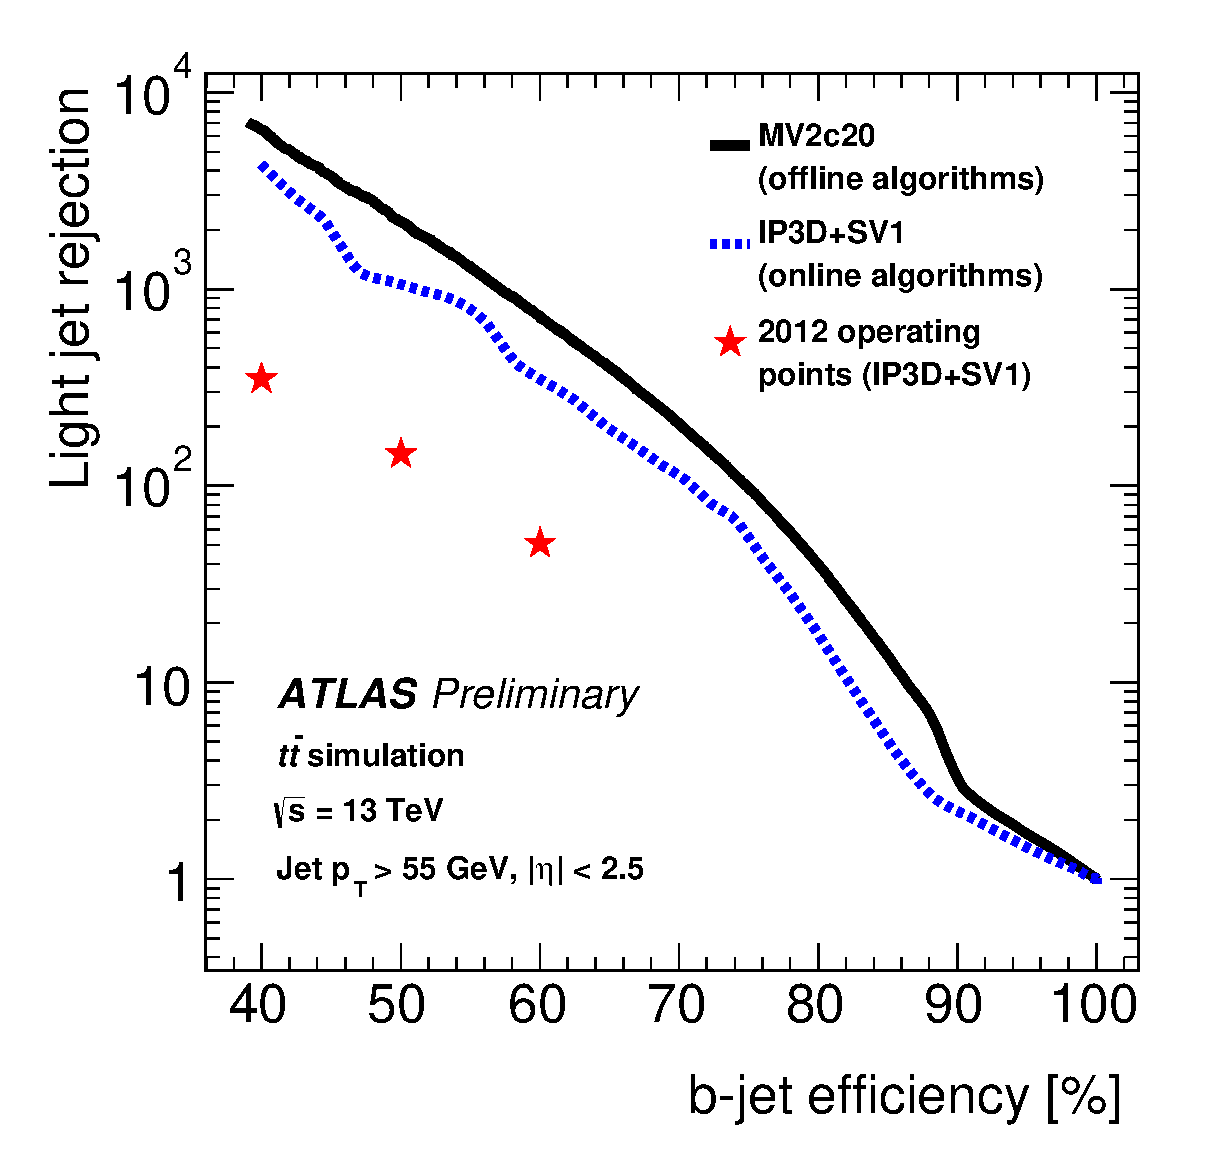
\includegraphics[width=0.48\linewidth, angle=0]{figs/Trigger/trig-bTrig_perf_light.eps}
    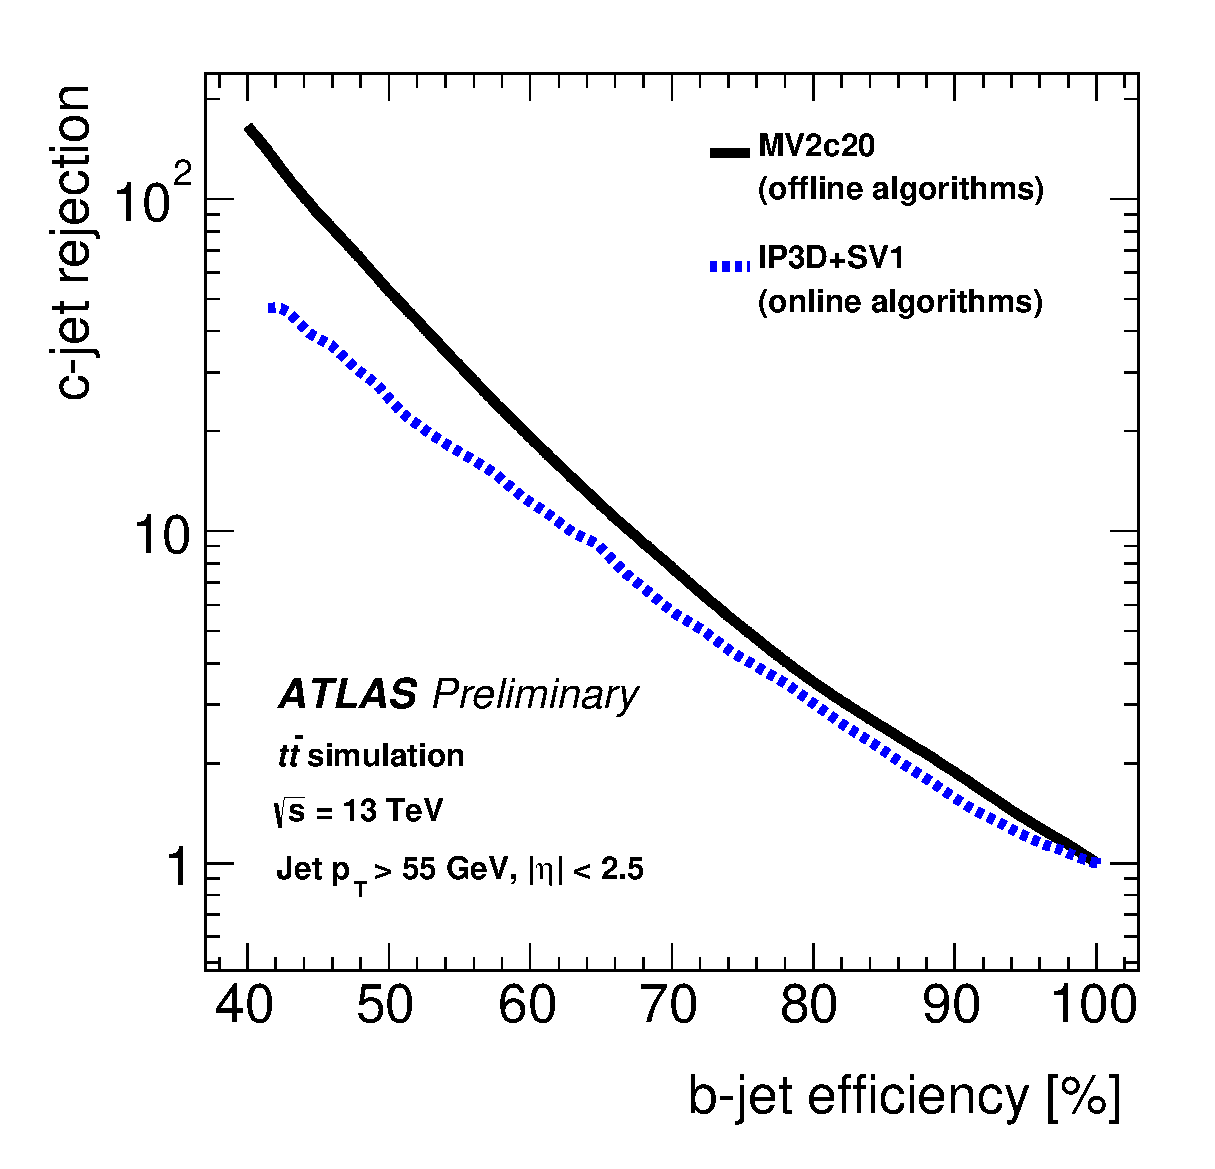
\includegraphics[width=0.48\linewidth, angle=0]{figs/Trigger/trig-bTrig_perf_charm.eps}
  \end{center}
  \caption{The expected $b$-jet efficiency of $b$-jet triggers with respect to (a) light-jet and (b) $c$-jet rejection
    in the case where the $b$-tagging algorithm used is MV2c20 (Black), IP3D+SV1 (Blue) and for the set-up used in Run-1 (red stars).}
  \label{fig:trig-bTrig_perf}
\end{figure}

There are few subtleties worth commenting on the $b$-jet trigger configuration, which affect decisions taken in this analysis.
One is that on this figure there are two lines corresponding to different $b$-tagging algorithms used in $b$-jet trigger;
IP3D+SV1 was used in 2015 data-taking,
whilst the MV2c20 was used in 2016 data-taking.
Another difference between 2015 and 2016 is the primary vertex finding algorithm used;
2016 data-taking employed a more complicated algorithm based on what is used offline, know as \verb|xPrmVtx|,
whilst in 2015 an algorithm using a simple histogram based approach was employed, known as \verb|EFHist|. 

Finally it is worth noting that there are  differences between online and offline $b$-tagging that will have an impact on what is to follow.
Firstly, coarser tracking information is available online, notably online tracks are not reconstructed from the whole range of the detector.
Secondly, a slightly different training setup is used for the multi-variate algorithm, mainly that a different fraction of $c$-jets were present in the training sample
(10\% offline vs. 20\% online).

In this analysis a double $b$-jet trigger is used,
\begin{center}
\verb|HLT_j150_bmc2c2060_split_j50_bmv2c2060_split|
\end{center}
which triggers on two jets with $p_T >$ 150 and 50 GeV respectively,
which have been $b$-tagged at the 60\% efficiency working point.

\newpage

\section{Efficiency Measurement of the $b$-Jet Trigger}
\label{sec:trig-bjet_eff}

Any part of the ATLAS detector framework needs to be understood and calibrated with data for use in an analysis;
and this includes the trigger which can have a large impact on the analysis.
In this section I discuss the strategy and results of the $b$-jet trigger efficiency measurement in 2016,
which is an important input to the low-mass channel of the di-$b$-jet analysis.

For clarity in this section I would like to make two definitions clear.
Online refers to any algorithms run or objects reconstructed at the trigger level,
offline refers to algorithms run after events have passed the trigger at the data-processing level. 

\subsection{Strategy}
The $b$-jet trigger is always used in tandem with offline $b$-tagging which is calibrated independently of the $b$-trigger.
Hence, to do this measurement whilst making use of the offline $b$-tagging calibrations already available,
$b$-jet trigger efficiency with respect to offline $b$-tagging, $\epsilon_{bTrig}$, is measured.
This is defined as the number of offline-tagged true $b$-jets that match an online-tagged trigger-jet
divided by the number of offline tagged $b$-jets that match a trigger jet.
Or to put this in an equation;
\begin{equation}
 \epsilon_{bTrig} = \frac{N(\text{Offline-tagged, online-tagged, true $b$-jets)}}{N(\text{Offline-tagged, trigger-matched, true $b$-jets)}}
\end{equation}
This quantity can be interpreted as the probability that a true $b$-jet is tagged at the trigger-level,
given that it there is a jet at the trigger level and that it would be $b$-tagged at the offline stage.

To measure $\epsilon_{bTrig}$ sample that has high $b$-jet purity is required,
such that jets uses to calculate this ratio are true $b$-jets.
It is also necessary to trigger on this sample in such a way that there is no bias from using $b$-tagging online;
or simply put the $b$-jet trigger cannot be used to select events.
The sample used to fill these criteria is a di-lepton $t\bar{t}$ sample containing a muon and an electron.
Top-quarks decay to a $W$-boson and a $b$-quark with almost 100\% branching ratio meaning that this sample provides a good source of $b$-quarks,
but also the electron and muon give a distinct signature which allows us to select this process with good purity and gives a non-$b$-jet object to trigger on.
The exact event selection is described below. 

The $b$-jet trigger efficiency is determined in data and is compared to the efficiency found in a 
simulated $t\bar{t}$ sample which is used to extrapolate the efficiency to 
higher jet-$p_T$ where the data-derived efficiency loses statistical precision.
The efficiency in data, including the simulation based extrapolation, can then be
compared to simulation to derive a Data/Monte-Carlo scale factor, which is used as the input to the analysis.


$\epsilon_{bTrig}$ and Data/Monte-Carlo scale factors are derived for all combinations of offline and online $b$-tagging working points.
However, only the process for the 70\% offline and 60\% online working point is shown
as this is set of working points used in this analysis.

\subsection{Datasets}
The data used for this analysis is the full 2016 ATLAS data-set.
In addition to the usual data-quality requirements applied,
as discussed in Section~\ref{sec:evtSel_GRL}\textit{(sec:evtSel\_GRL)},
a $b$-jet trigger aware Good Run List (GRL)
\footnote{A GRL is effectively a list of lumi-blocks that pass certain data-quality requirements.
 As mentioned in the text a further discussion is held here in Section~\ref{sec:evtSel_GRL}\textit{(sec:evtSel\_GRL)}}
applies the requirement that the online beamspot $z$-position is within 2mm of the origin in Periods A-I of the data.
This means that the data-set contains 24.5~\ifb of data.
A discussion of the requirement for this GRL is in Section~\ref{sec:trig-inv}. 

For the simulated $t\bar{t}$ sample, the generation is performed with
a Powheg-Box v2~\cite{trig-powheg} generator with the CT10 PDF sets in the matrix element calculations.
Also considered is a simulated single-top sample;
electroweak t-channel, s-channel and $Wt$-channel single top-quark events are generated using the Powheg-Box v1 generator.
This generator uses the 4-flavour scheme for the NLO matrix elements calculations together with the fixed four-flavour PDF set CT10f4.
%For all top processes, top-quark spin correlations are preserved (for t-channel, top quarks are decayed using MadSpin[10a]).
For both processes the parton shower, fragmentation, and the underlying event are simulated using Pythia6.428~\cite{trig-pythia6} with the CTEQ6L1~\cite{trig-CTEQ6L1} PDF sets
and the corresponding Perugia 2012 tune (P2012)~\cite{trig-perugia}.
The top mass is set to 172.5 GeV.
The EvtGen v1.2.0 program~\cite{trig-evtGen} is used for properties of the bottom and charm hadron decays. 
\newpage

\subsection{Event Selection}
\label{sec:trig-evtSel}

A high-purity sample of $b$-jets is selected using a di-lepton $t\bar{t}$ selection.

\noindent
The event selection is summarised as follows:

\begin{itemize}
\item The event fired a single lepton bperf trigger which are:
    \begin{itemize}[label={$-$}]
      \item\verb|HLT_mu26_imedium_2j35_bperf|
      \item\verb|HLT_e26_tight_iloose_2j35_bperf|
      \item\verb|HLT_e26_lhtight_iloose_2j35_bperf|
    \end{itemize}
\item At least 1 medium muon: $\pT>25~\GeV$, which has no jet within a $\Delta R$ of 0.4.
\item At least 1 medium electron: $\pT>25~\GeV$.
\item 2 offline $b$-tagged jets, defined as:
   \begin{itemize}[label={$-$}]
     \item Offline R=0.4 anti-$k_T$ jets.
     \item $\pT>35~\GeV$ and $|\eta|<2.5$.
     \item Offline $b$-tagged at the 85\%~operating point.
     \item Jet must be matched to a trigger-jet.
    \end{itemize}
\end{itemize}
\vspace{1em}

Descriptions of the object-definitions of muons, electrons, jets and $b$-tagged can be found in
Sections~\ref{sec:object_muon}\textit{(sec:object\_muon)},~\ref{sec:object_electron}\textit{(sec:object\_elec)},~\ref{sec:object_jet}\textit{(sec:object\_jet)}
and \ref{sec:object_bjet}\textit{(sec:object\_bjet)} respectively.
Online trigger jets are matched exclusively to offline jets using $\Delta R$ matching, requiring for a match the jets must have $\Delta R<0.6$.

The triggers used are bperf trigger, which are special triggers used in data-taking specifically for monitoring the $b$-jet trigger performance.
They fire if a muon or an electron with $\pT > 26$~\GeV is reconstructed at the trigger level.
The bperf triggers then run the online $b$-tagging algorithm on all trigger jets with $|\eta|<2.5$ and
$p_{T}>35$~\GeV without performing any cuts on the output of the multi-variate algorithm; ensuring there is no bias in the efficiency measurement. 


\newpage

\subsection{The Initial Problem}
\label{sec:trig-initProb}

To give context to the following section;
the first discussion will be what was first observed when measuring the $b$-jet efficiency.
To show the problems observed clearly, in this section original event selection is replicated;
hence  no $b$-jet trigger aware GRL is applied, offline jets are not required to match a trigger jet in the denominator
and the triggers required are single lepton triggers without the additional $b$-perf functionality
\footnote{Specifically HLT\_mu26\_imedium, HLT\_e26\_tight\_iloose and HLT\_e26\_lhtight\_iloose. }.
In addition, for this and the following two sections simulation refers to $t\bar{t}$ only,
but it will be shown later that the effect of single-top production is small so the conclusions here are still valid. 

Figure~\ref{fig:trig-Full_noGRL_eff_noHLTMatch} shows $\epsilon_{bTrig}$ against jet-\pT~and jet-$\eta$;
the efficiency in data is substantially below the efficiency expected from simulation and shows a clear shape in jet-$\eta$ distributions.
This substantial difference need to be investigated and understood. 

\begin{figure}[!ht]
  \begin{center}
    \captionsetup[subfigure]{aboveskip=0pt,justification=centering}
    \subcaptionbox{Jet-\pT}{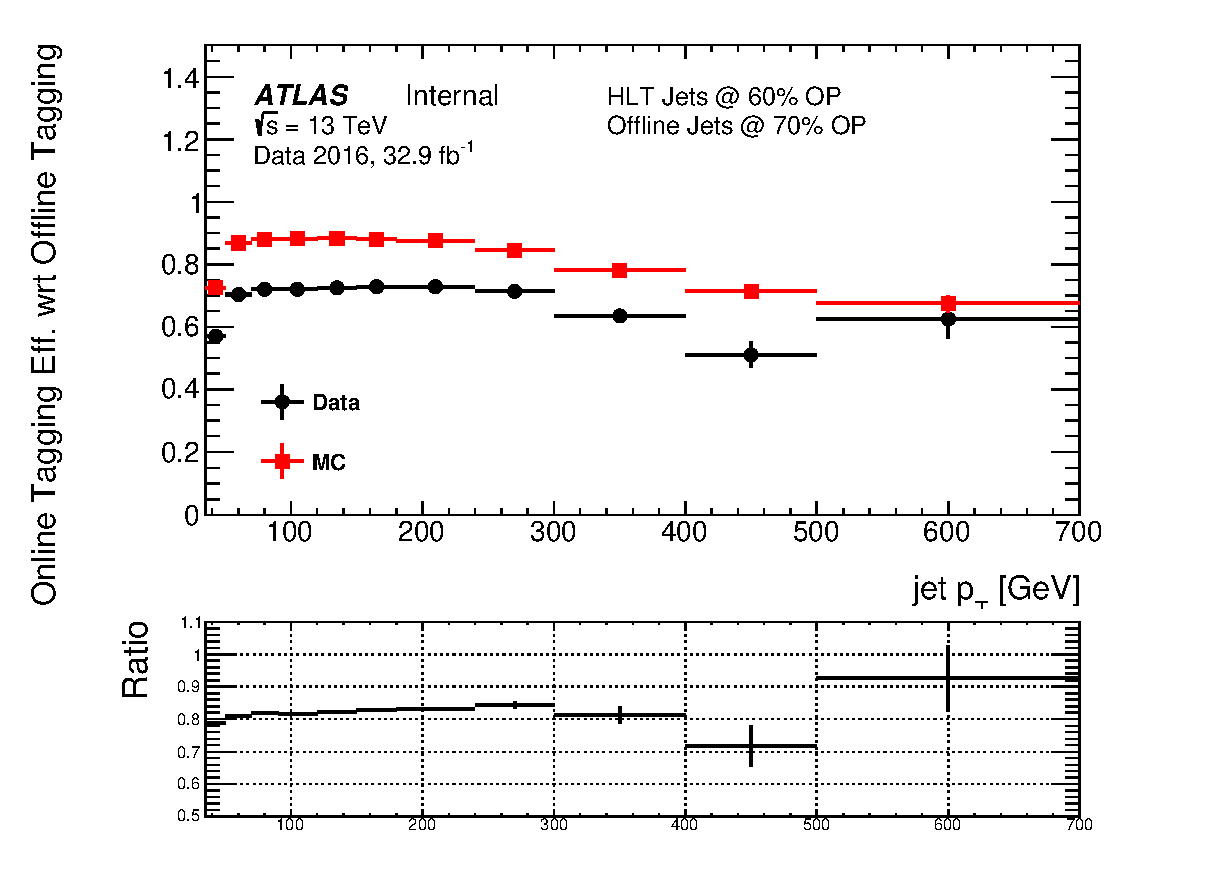
\includegraphics[width=0.48\linewidth, angle=0]{figs/trigger/Full_noGRL_eff_noHLTMatch_jetPt.eps} }
    \subcaptionbox{Jet-$\eta$}{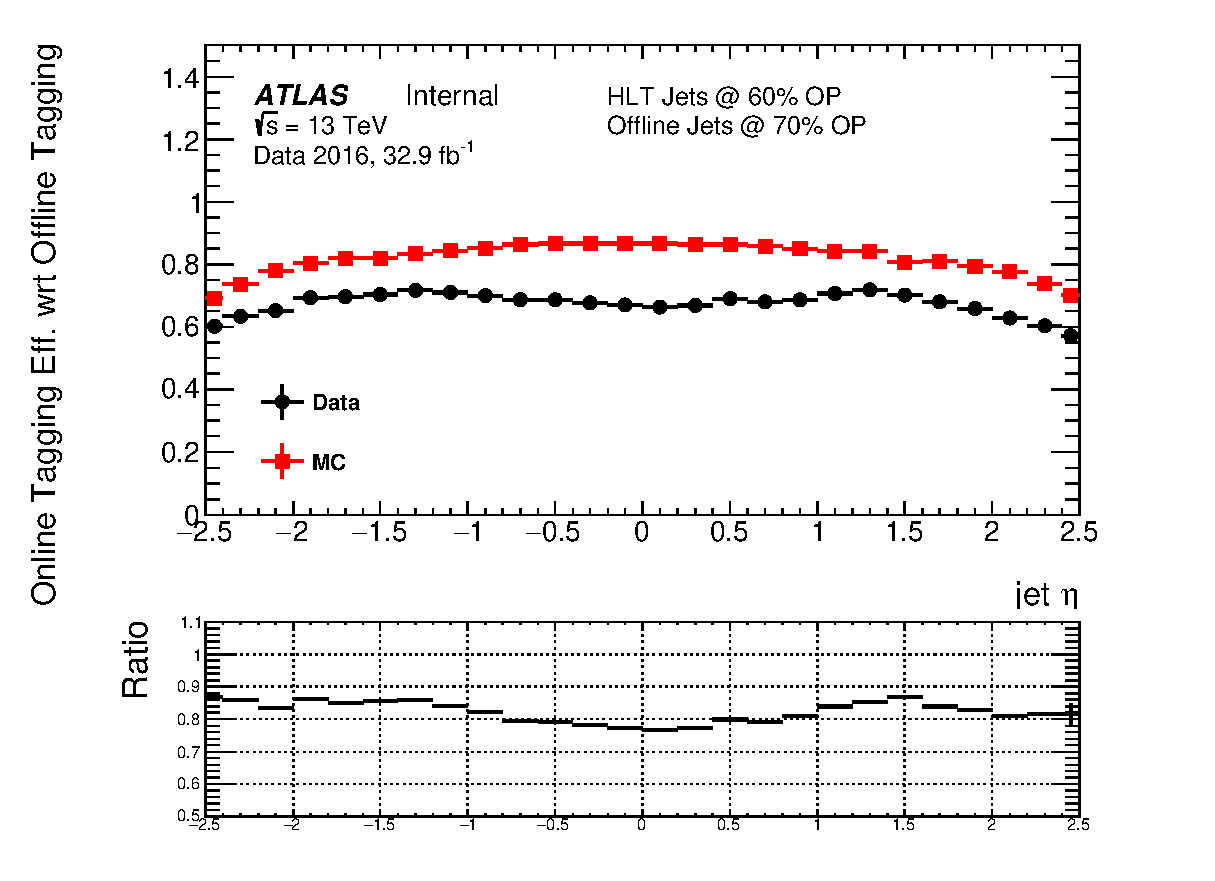
\includegraphics[width=0.48\linewidth, angle=0]{figs/trigger/Full_noGRL_eff_noHLTMatch_jetEta.eps}}
  \end{center}
  \caption{The 60\% $b$-jet trigger efficiency with respect to an offline 70\% operating point tag
    for Data (black) and simulation (red) against jet-\pT~(a) and jet-$\eta$ (b).
    The $b$-trigger aware GRL is not applied and trigger matching is not required.}
  \label{fig:trig-Full_noGRL_eff_noHLTMatch}
\end{figure}

\subsection{Investigation}
\label{sec:trig-inv}

Given the disagreements between data and simulation shown above
a number of cross-checks were performed to understand this discrepancy,
including checking for performance dependence on period,
detector performance, pile-up conditions and online beamspot position.
In this section, I summarise the results of the investigation
and our understanding of the $b$-trigger performance in 2016 data.
For this, set-up as described in \ref{sec:trig-evtSel} is used
with the exception that $b$-jet aware GRL is not applied to allow us to see the problems clearly.

The major problem that was discovered to be causing the large discrepancies was related to Primary Vertex finding.
As described above, in 2016 data an algorithm known as \verb|xPrmVtx| was used to find the primary vertex.
It has since been uncovered that there was a bug in the code used to implement this algorithm;
effectively different co-ordinates were used by different components of the code.
Online tracks passed to \verb|xPrmVtx| use position with respect to online beam-spot position,
where the \verb|xPrmVtx| algorithm assumed track position with respect to the origin.
This means that when the online beamspot $z$-position is far from from the origin,
a vertex with position at the origin is passed to the $b$-tagging algorithms,
This leads to sub-optimal performance, as will be shown below.
For ease of reading online beamspot $z$-position is henceforth referred to as $z_{bs}^{online}$.  

The exact setup for the $b$-jet trigger has changed as data has taken, to respond to performance issues as they are noticed and patches are applied
As such the relevant conditions of the $b$-jet trigger can be split into three regions of data-taking, which I will refer to as epochs.
The effect of \verb|xPrmVtx| returning a dummy vertex on $b$-jet trigger performance is different in each of these epochs,
the details are summarised Table~\ref{tab:trig-epochs}.
As a result of these differences in trigger performance, each epoch is now considered independently.

\begin{table}[!htb]
  \begin{tabular}{ | c || c | c | c |}
    \hline			
    Epoch & Runs & Periods & Effect if no \verb|xPrmVtx| PV is found \\ \hline
    1 & \parbox[t]{2.5cm} {296939-300571,\\ 300655 \\}  & A,B(part)             & \parbox[t]{5cm} {\hspace{1mm}An invalid vertex is passed to the online b-tagging } \\
    \hline
    2 & \parbox[t]{2.5cm} {300600,\\ 300784-308084\\}  & B(part),C,D,E,F,G,I,J & \parbox[t]{5cm} {\hspace{1mm}The b-jet trigger is not fired\\ } \\
    \hline
    3 & \parbox[t]{2.5cm} {309331-311481\\}       & K,L                     & \parbox[t]{5cm} {\hspace{1mm}A back-up primary vertex \\ finding algorithm is used.\\} \\
    \hline
  \end{tabular}
  \vspace{10pt}
  \caption{A table describing the effect of not finding a valid xPrmVtx primary vertex on different epochs of data.}
  \label{tab:trig-epochs}
\end{table}
%For Epoch 1, the $\epsilon_{bPerf}$ is 100\% as shown in Figure~\ref{fig:Epoch1_bperf} for Period A.Figure~\ref{fig:Epoch1_eff} shows the $\epsilon_{bTrig}$ in Epoch 1,
Firstly let us consider Epoch 1;
Figure~\ref{fig:Epoch1_eff}(a) shows that efficiency against jet-\pT~is ~80-90\% of that in simulation, similar to that shown in the previous section.
However, Figure~\ref{fig:Epoch1_eff}(b) shows that $\epsilon_{bTrig}$ in Epoch 1 has a strong dependence of  $z_{bs}^{online}$;
when  $z_{bs}^{online}$ is close to zero $\epsilon_{bTrig}$ in data and simulation are comparable
\footnote{In simulation the  $z_{bs}^{online}$ is always set to zero.}
but as $|z_{bs}^{online}|$ increases efficiency falls off steeply.
To understand this performance the variable `vertex class' is studied, which is defined as 0 when a valid \verb|xPrmVtx| vertex is found and 1 if not.
Figure~\ref{fig:Epoch1_vtxClass}(a) shows that when an \verb|xPrmVtx| vertex is found $\epsilon_{bTrig}$ is reasonably high ($\sim$ 0.8) and is comparable between data and simulation (within 5\%),
whilst if no valid \verb|xPrmVtx| vertex is found then efficiency is very low in both simulation and data.
However, Figure~\ref{fig:Epoch1_vtxClass}(b) shows that a \verb|xPrmVtx| is found in simulation in $> 99$ \% of the jets,
whilst in data there is $\sim$ 16\% of events where no \verb|xPrmVtx| is found.
Hence, combining the information in Table~\ref{tab:trig-epochs}, Figure~\ref{fig:Epoch1_eff} and Figure~\ref{fig:Epoch1_vtxClass}
it can be concluded that in Epoch 1 in events where the  $|z_{bs}^{online}|$ is far from 0
then \verb|xPrmVx| returns an invalid vertex which results in a low $\epsilon_{bTrig}$, explaining the data/simulation differences in Epoch 1. 

\begin{figure}[!ht]
  \begin{center}
    \captionsetup[subfigure]{aboveskip=0pt,justification=centering}
    \subcaptionbox{Jet-\pT}{\includegraphics[width=0.48\linewidth, angle=0]{figs/Trigger/btrigger_old/Epoch1_trigReq_eff_jetPt.pdf} }
    \subcaptionbox{ $z_{bs}^{online}$}{\includegraphics[width=0.48\linewidth, angle=0]{figs/Trigger/btrigger_old/Epoch1_trigReq_eff_bs_online_vz.pdf} }
  \end{center}
  \caption{The 60\% $b$-jet trigger efficiency with respect to an offline 70\% operating point tag
    for data from Epoch 1 (black) and simulation (red) against jet-\pT~(a) and online beamspot $z$-position (b).
    The $b$-jet trigger aware GRL has not been applied.}
  \label{fig:Epoch1_eff}
  \begin{center}
    \captionsetup[subfigure]{aboveskip=0pt,justification=centering}
    \subcaptionbox{$\epsilon_{bTrig}$ against Vertex Class}{\includegraphics[width=0.48\linewidth, angle=0]{figs/Trigger/btrigger_old/Epoch1_trigReq_eff_vtxClass.pdf}}
    \subcaptionbox{Freq. of Offline Jets against Vertex Class}{\includegraphics[width=0.48\linewidth, angle=0]{figs/Trigger/btrigger_old/Epoch1_trigReq_nOff_vtxClass.pdf}}
    \end{center}
  \caption{(a) The 60\% $b$-jet trigger efficiency with respect to an offline 70\% operating point tag
    and  (b) the number of offline jets passing 70\% operating point tag and matching a HLT trigger jet
    against vertex class for data from Epoch 1 (black) and simulation (red). 
    The $b$-jet trigger aware GRL has not been applied.}
    \label{fig:Epoch1_vtxClass}
\end{figure}

\FloatBarrier


%\begin{figure}[!ht]
%\begin{center}
%  \includegraphics[width=0.47\linewidth, angle=0]{figs/Trigger/btrigger_old/Epoch1_trigReq_bPerfEff_jetPt.pdf}
%  \includegraphics[width=0.47\linewidth, angle=0]{figs/Trigger/btrigger_old/Epoch1_trigReq_bPerfEff_bs_online_vz.pdf}
%\end{center}
%\caption{$b$-perf efficiency, $\epsilon_{bPerf}$, for data from Period A (black) and simulation (red) against jet-pT~(left) and online beamspot $z$-position (right).}
%\label{fig:Epoch1_bperf}
%\end{figure}

In Epoch 2, there is a similar problem to Epoch 1, but there is a subtle difference which requires us to look at this region in a
different way.
As in Epoch 1, when  $z_{bs}^{online}$ is far from zero then a \verb|xPrmVtx| PV is not found.
However in Epoch 2 this means that the  $b$-jet trigger was discovered to falsely terminate whilst processing the event,
meaning that there are no online $b$-jets are available in the event, and therefore the trigger will not fire.
However, the additional complication compared to Epoch 1 is this means that the  $b$-perf triggers used to measure the efficiency
are also not fired when no valid \verb|xPrmVtx| PV is available.
Hence, measuring $\epsilon_{bTrig}$ using the set-up as described will not capture the cases where a valid \verb|xPrmVtx| PV is found
and thus $\epsilon_{bTrig}$ should be consistent in data and simulation;
Figure~\ref{fig:Epoch2_eff} shows the $\epsilon_{bTrig}$ is measured in data to be in agreement with simulation within 5\%.


For Epoch 2, in addition to measuring $\epsilon_{bTrig}$ it is necessary
to also account for the cases when a false \verb|xPrmVtx| PV is found.
This is done by measuring the $b$-perf efficiency, $\epsilon_{bPerf}$,
the efficiency that there is a valid primary vertex in the event.
$\epsilon_{bPerf}$ is calculated by dividing the number of events that pass the trigger
\verb|HLT_mu26_imedium_2j35_bperf| by the number that pass the trigger \verb|HLT_mu26_imedium|,
such that the denominator has no $b$-trigger dependency so is unaffected by \verb|xPrmVtx| PV.
This is an event level quantity and as such is measured with respect other event level quantity, such as leading jet-\pT.
Figure~\ref{fig:Epoch2_bperf} shows that:
$\epsilon_{bPerf}$ has a data/simulation ratio of around 80\%  which is similar to that in Section~\ref{sec:trig-initProb} and
$\epsilon_{bPerf}$ shows similar behaviour with respect to  $z_{bs}^{online}$ as observed in Epoch 1.
Finally it is observed that $\epsilon_{bPerf}$ has a lower efficiency at smaller values of absolute leading jet-$\eta$;
this is due to the fact that at high-$\eta$ tracks have a larger error on the longitudinal impact parameter, $z_0$,
meaning that the mis-match of co-ordinates can in the \verb|xPrmVtx| algorithm is covered by the errors, mitigating this issue.
This effect must be accounted for in the final efficiency measurement.

\begin{figure}[!ht]
\begin{center}
  \captionsetup[subfigure]{aboveskip=0pt,justification=centering}
  \subcaptionbox{Jet-\pT}{\includegraphics[width=0.47\linewidth, angle=0]{figs/Trigger/btrigger_old/Epoch2_trigReq_eff_jetPt.pdf}}     
  \subcaptionbox{Jet-$\eta$}{\includegraphics[width=0.47\linewidth, angle=0]{figs/Trigger/btrigger_old/Epoch2_trigReq_eff_bs_online_vz.pdf}}
  %\subcaptionbox{??}{\includegraphics[width=0.47\linewidth, angle=0]{figs/Trigger/btrigger_old/Epoch2_trigReq_eff_jetEta.pdf}} \\
  %\subcaptionbox{??}{\includegraphics[width=0.47\linewidth, angle=0]{figs/Trigger/btrigger_old/Epoch2_trigReq_eff_vtxClass.pdf}}
\end{center}
\caption{The 60\% $b$-jet trigger efficiency with respect to an offline 70\% operating point tag
         for data from epoch 2 (black) and simulation (red) against jet-\pT~(a), jet-$\eta$ (b) and online beamspot $z$-position (c).}
\label{fig:Epoch2_eff}
\begin{center}
  \captionsetup[subfigure]{aboveskip=0pt,justification=centering}
  \subcaptionbox{Leading Jet-\pT}{\includegraphics[width=0.47\linewidth, angle=0]{figs/Trigger/btrigger_old/Epoch2_trigReq_bPerfEff_jetPt.pdf}}
  \subcaptionbox{$z_{bs}^{online}$}{\includegraphics[width=0.47\linewidth, angle=0]{figs/Trigger/btrigger_old/Epoch2_trigReq_bPerfEff_bs_online_vz.pdf}}
  \subcaptionbox{Leading Jet-$\eta$}{\includegraphics[width=0.47\linewidth, angle=0]{figs/Trigger/btrigger_old/Epoch2_trigReq_bPerfEff_jetEta.pdf}}
\end{center}
\caption{$b$-perf efficiency, $\epsilon_{bPerf}$, for data from Epoch 2 (black) and simulation (red) against leading-jet \pT~(a), online beamspot $z$-position (b) and leading jet-$\eta$ (c).}
\label{fig:Epoch2_bperf}
\end{figure}
Epoch 3, when no \verb|xPrmVtx| PV is found then a backup PV finding algorithm is used, known as \verb|EFHist|, which finds the PV through a basic histogramming of the tracks,
the simplicity of the algorithm means that a PV can be found as long as 1 track is present.
Figure~\ref{fig:Epoch3_eff} shows $\epsilon_{bTrig}$ for Epoch 3 for jet-\pT, jet-$\eta$,  $z_{bs}^{online}$ and vertex class (as defined above).
In Epoch 3 $\epsilon_{bTrig}$ measured in data is within 5\% of simulation and there is no shape difference between the two with respect to jet-$\eta$.
In addition it is shown that in Epoch 3 there is no strong dependence on  $z_{bs}^{online}$,
and that efficiency in data is consistent if a valid \verb|xPrmVtx| vertex or not (vertex class = 0 or 1 respectively).
This demonstrates that the success of the backup vertex approach.

\begin{figure}[!ht]
\begin{center}
  \captionsetup[subfigure]{aboveskip=0pt,justification=centering}
  \subcaptionbox{Jet-\pT}{\includegraphics[width=0.47\linewidth, angle=0]{figs/Trigger/btrigger_old/Epoch3_trigReq_eff_jetPt.pdf}}
  \subcaptionbox{Jet-$\eta$}{\includegraphics[width=0.47\linewidth, angle=0]{figs/Trigger/btrigger_old/Epoch3_trigReq_eff_jetEta.pdf}} \\
  \subcaptionbox{$z_{bs}^{online}$}{\includegraphics[width=0.47\linewidth, angle=0]{figs/Trigger/Epoch3_eff_bs_online_vz.eps}}
  \subcaptionbox{Vertex Class}{\includegraphics[width=0.47\linewidth, angle=0]{figs/Trigger/btrigger_old/Epoch3_trigReq_eff_vtxClass.pdf}}
\end{center}
\caption{The 60\% $b$-jet trigger efficiency with respect to an offline 70\% operating point tag
  for data from Epoch 3 (black) and simulation (red) against (a) jet-\pT, (b) jet-$\eta$,
  (c) online beamspot $z$-position and (d) vertex class.}
\label{fig:Epoch3_eff}
\end{figure}

\FloatBarrier

\subsection{Solution: $b$-Jet Trigger GRL}
\label{sec:trig-inv}

To summarise, in the previous section it is shown that at large values of absolute online beamspot $z$-position
the measured $\epsilon_{bTrig}$ in Epoch 1 and $\epsilon_{bPerf}$ in Epoch 2 is lower in data than in MC, due to poor \verb|xPrmVtx| PV finding performance.
In Epoch 3 there is reasonable data/simulation agreement due to the use of a backup vertex finding algorithm. 

The solution employed is to apply a $b$-jet trigger aware GRL 
that removes events where the  absolute  $z_{bs}^{online}$ of greater than 2mm in Epoch 1 and 2,
such that the events with low efficiency are removed.
The cost of this approach is the luminosity of our data-set is reduced, specifically the data-set falls from  32.9~\ifb to 24.3~\ifb.
However there are three key reasons why use of a $b$-jet trigger GRL was chosen over simply applying an overall efficiency.
Firstly, as there is no beamspot position distribution in simulation it is not clear that kinematics of events at high  $z_{bs}^{online}$ can be well understood and modelled;
the sculpting of the efficiency with respect to jet-$\eta$ is an example of this.
Secondly, the efficiencies are quite low at high beamspot $z$-position,
so the loss in luminosity x acceptance is relatively small
and finally the use of a GRL means a more realistic estimate of the actual luminosity used in an analysis is used. 

For the choice of which value of beamspot $z$ position to use for in the GRL,
it was required to select the widest cut where the efficiency had not significantly declined,
such that as much luminosity as possible is retained, while removing most of the affected region.
This \SI{2}{\mm} cut was chosen from examining Figure~\ref{fig:Epoch1_eff}(b) and Figure~\ref{fig:Epoch2_bperf}(b),
and from studying a variety of cuts from \SI{2}{\mm} to \SI{1}{\mm}.

After the GRL is applied, $\epsilon_{bTrig}$ for Region 1 becomes approximately 90-95\% of the efficiency measured in simulation,
as shown in Figure~\ref{fig:Epoch1_bslt2mm_eff},
and $\epsilon_{bPerf}$ for Region 2 becomes approximately 95\% of the efficiency measured in simulation,
as shown in Figure~\ref{fig:Epoch2_bslt2mm_bperf}. 

\begin{figure}[!ht]
  \begin{center}
    \captionsetup[subfigure]{aboveskip=0pt,justification=centering}
    \subcaptionbox{Jet-\pT}{\includegraphics[width=0.47\linewidth, angle=0]{figs/Trigger/btrigger_old/Epoch1_GRL_bslt2mm_trigReq_eff_jetPt.pdf} }
    \subcaptionbox{Jet-$\eta$}{\includegraphics[width=0.47\linewidth, angle=0]{figs/Trigger/btrigger_old/Epoch1_GRL_bslt2mm_trigReq_eff_jetEta.pdf}}
  \end{center}
  \caption{The 60\% $b$-jet trigger efficiency with respect to an offline 70\% operating point tag
    for data from Region 1 (black) and simulation (red) against jet-\pT~(a) and jet-$\eta$ (b).
    The $b$-jet trigger aware GRL has been applied.}
  \label{fig:Epoch1_bslt2mm_eff}
  \begin{center}
    \captionsetup[subfigure]{aboveskip=0pt,justification=centering}
    \subcaptionbox{Leading Jet-\pT}{\includegraphics[width=0.47\linewidth, angle=0]{figs/Trigger/btrigger_old/Epoch2_GRL_bslt2mm_trigReq_bPerfEff_jetPt.pdf} }
    \subcaptionbox{Leading Jet-$\eta$}{\includegraphics[width=0.47\linewidth, angle=0]{figs/Trigger/btrigger_old/Epoch2_GRL_bslt2mm_trigReq_bPerfEff_jetEta.pdf}}
  \end{center}
  \caption{$b$-perf efficiency, $\epsilon_{bPerf}$, for data from Region 2 (black) and simulation (red) against leading (a) jet-\pT~and (b) jet-$\eta$.
    The $b$-jet trigger aware GRL has been applied.}
  \label{fig:Epoch2_bslt2mm_bperf}
\end{figure}

\newpage

Figure~\ref{fig:Full_bslt2mm_bperf} and ~\ref{fig:Full_bslt2mm_eff} shows measured
$\epsilon_{bPerf}$ and $\epsilon_{bTrig}$
for the full 2016 data-set, combining Regions 1, 2 and 3,
with the $b$-jet trigger aware GRL applied.
This represents the raw observed data/simulation efficiencies when the full event selection has been applied.

\begin{figure}[!ht]
  \begin{center}
    \captionsetup[subfigure]{aboveskip=0pt,justification=centering}
    \subcaptionbox{Jet-\pT}{\includegraphics[width=0.47\linewidth, angle=0]{figs/Trigger/btrigger_old/Full_GRL_bslt2mm_trigReq_eff_jetPt.pdf}}
    \subcaptionbox{Jet-$\eta$}{\includegraphics[width=0.47\linewidth, angle=0]{figs/Trigger/btrigger_old/Full_GRL_bslt2mm_trigReq_eff_jetEta.pdf}}\\
    \subcaptionbox{$z_{bs}^{online}$}{\includegraphics[width=0.47\linewidth, angle=0]{figs/Trigger/btrigger_old/Full_GRL_bslt2mm_trigReq_eff_bs_online_vz.pdf}}
    \subcaptionbox{Vertex Class}{\includegraphics[width=0.47\linewidth, angle=0]{figs/Trigger/btrigger_old/Full_GRL_bslt2mm_trigReq_eff_vtxClass.pdf}}
  \end{center}
  \caption{The 60\% $b$-jet trigger efficiency with respect to an offline 70\% operating point tag
    for the full 2016 data-set (black) and simulation (red) against jet-\pT~(a), jet-$\eta$ (b), online beamspot $z$-position (c) and vertex class (d).}
  \label{fig:Full_bslt2mm_eff}
  \begin{center}
    \captionsetup[subfigure]{aboveskip=0pt,justification=centering}
    \subcaptionbox{Leading Jet-\pT}{\includegraphics[width=0.47\linewidth, angle=0]{figs/Trigger/btrigger_old/Full_GRL_bslt2mm_trigReq_bPerfEff_jetPt.pdf}}
    \subcaptionbox{Leading Jet-$\eta$}{\includegraphics[width=0.47\linewidth, angle=0]{figs/Trigger/btrigger_old/Full_GRL_bslt2mm_trigReq_bPerfEff_jetEta.pdf}}
  \end{center}
  \caption{$b$-perf efficiency, $\epsilon_{bPerf}$, for the full 2016 data-set (black) and simulation (red) against (a) leading jet-\pT~and (b) jet-$\eta$.
    The $b$-jet trigger aware GRL has been applied.}
  \label{fig:Full_bslt2mm_bperf}
\end{figure}
  

\FloatBarrier
\newpage

\subsection{Efficiency Measurement and Systematic Derivation}
In the previous two sections it has been shown that when applying a $b$-jet aware GRL,
the $b$-jet trigger performance is understood and the data/simulation agreement is within 5\%.
In this section the measurement of data efficiency and data/simulation scale factors (SFs)
and associated systematics to account for the 5\% are described.

As discussed above, there are two factors considered in this section.
Firstly there is the $\epsilon_{bTrig}$ measurement
that accounts for differences in online and offline $b$-tagging given that a valid primary vertex has been found.
Sections~\ref{sec:trig-purity}~to~\ref{sec:trig-highPtExtrap} describes the derivation of a set of systematics and corrections to the raw measurement
and Section~\ref{sec:trig-jetLevelEff} presents the final measurement, which is applied as a jet-level efficiency in the final analysis.
Secondly, in Section~\ref{sec:trig-eventLevelEff}, is a description the measurement of the $\epsilon_{bPerf}$ that accounts
for the efficiency of finding a valid primary vertex and the relevant systematics, which is applied as an event level efficiency.

In this section describing the final measurement, the full 2016 data set is used,
the simulated ${t\bar{t}}$ sample includes single-top processes
and the full event selection from Section~\ref{sec:trig-evtSel} is applied.

% This section got cut and moved to jetLevelEff
%\subsubsection{$\eta$ Dependence on Efficiency}
%\label{sec:trig-etaDep}
%\begin{figure}[!ht]
%  \begin{center}
%    \includegraphics[width=0.47\linewidth, angle=0]{figs/Trigger/btrigger_old/Full_GRL_bslt2mm_trigReq_eff_jetPt.pdf}
%    \includegraphics[width=0.47\linewidth, angle=0]{figs/Trigger/btrigger_old/Full_GRL_bslt2mm_trigReq_eff_jetEta.pdf}
%  \end{center}
%  \caption{The 60\% $b$-jet trigger efficiency with respect to an offline 70\% operating point tag
%    for data from Periods A-L (black) and simulation (red) against jet-\pT~(a), jet-$\eta$ (b).}
%  \label{fig:Full_bslt2mm_eff_eta}
%\end{figure}

\subsubsection{Purity Error}
\label{sec:trig-purity}

It is known that despite the strict event selection there will inevitably be non b-jet contamination in our sample.
To estimate the b-jet purity simulation is used, where the true flavour of the jet is available.
Jets as categorised as true $b$-jets, meaning that a $B$-hadron was found with in a cone of R = 0.4, or true non-b-jets if not.
Then distributions for inclusive jets to the truth matched b-jets in the simulation sample are compared.
Figure~\ref{fig:Purity} shows the b-jet purity for jet-\pT~and jet-$\eta$;
showing that the b-jet purity is $>$ 95\% up to jet-\pT$\sim$300~\GeV~and $>$ 90\% for higher values of jet-\pT.

To estimate the effect of these impurities on the efficiency measurement simulation is again used.
Firstly, the efficiency in our nominal inclusive simulation is compared
to the efficiencies if only true-b-jets or true non-b-jets are selected,
this is shown if Figure~\ref{fig:Eff_Purity}(a).
The ratio is applied as a correction to the final efficiency measurement.
Then any mismodelling of the  $b$-jet fraction is simulation is also considered,
to account for this the efficiency for the simulated inclusive sample is compared to the efficiency when the non b-jet content has been doubled, as shown in Figure~\ref{fig:Eff_Purity}(b).
The maximum difference from the efficiency measured in the inclusive simulated sample and the cases
where there is only true b-jets and where the non b-jet content has been doubled,
shown in the two ratio plots in Figure~\ref{fig:Eff_Purity}, is taken as a symmetric systematic.

\begin{figure}[!ht]
  \begin{center}
    \captionsetup[subfigure]{aboveskip=0pt,justification=centering}
    \subcaptionbox{Jet-\pT}{\includegraphics[width=0.47\linewidth, angle=0]{figs/Trigger/btrigger_old/PurityMC_jetPt.pdf}}
    \subcaptionbox{Jet-$\eta$}{\includegraphics[width=0.47\linewidth, angle=0]{figs/Trigger/btrigger_old/PurityMC_jetEta.pdf}}
  \end{center}
  \caption{A comparison of offline jets tagged at the 70\% operating point
    for inclusive jets (red) and truth-matched b-jets (blue)
    against jet-\pT~(a) and jet-$\eta$ (b) in a simulated $t\bar{t}$ sample.}
  \label{fig:Purity}
  \begin{center}
    \captionsetup[subfigure]{aboveskip=0pt,justification=centering}
    \subcaptionbox{}{\includegraphics[width=0.47\linewidth, angle=0]{figs/Trigger/btrigger_old/EffMC_jetPt_trueB.pdf}}
    \subcaptionbox{}{\includegraphics[width=0.47\linewidth, angle=0]{figs/Trigger/btrigger_old/EffMC_jetPt_2nonB.pdf}}
  \end{center}
  \caption{The 60\% $b$-jet trigger efficiency with respect to an offline 70\% operating point tag
    for inclusive jets (black) compared to truth matched b-jets and non b-jets (a) and the case where non b-jet content has been doubled (b) for a simulated $t\bar{t}$ sample.
    The lower panel in both plots show the ratio to the inclusive efficiency.
  }
  \label{fig:Eff_Purity}
\end{figure}

\subsubsection{Non-b-jet trigger efficiency error}
\label{sec:trig-lightTrigEff}

As one would expect and as shown in left plot of Figure~\ref{fig:Eff_Purity}, non b-jets (shown in blue) have a different b-jet trigger efficiency to that of b-jets.
However the exact efficiency is not known well in data and could be mismodelled in simulation.
To account for this uncertainty the nominal efficiency in simulation is compared
to the cases where the non-b-jet efficiency has been halved and doubled in simulation, as shown in Figure~\ref{fig:Eff_LTrigEff}.
When doubling the non-b-jet trigger efficiency this is limited at the upper end to being no greater than the true b-jet trigger efficiency.
The maximum bin-by-bin difference between the nominal and the two cases, as shown in the two ratio plots, is taken as a systematic.

\begin{figure}[!ht]
  \begin{center}
    \captionsetup[subfigure]{aboveskip=0pt,justification=centering}
    \subcaptionbox{}{\includegraphics[width=0.47\linewidth, angle=0]{figs/Trigger/btrigger_old/effMC_jetPt_lowLTrigEff.pdf}}
    \subcaptionbox{}{\includegraphics[width=0.47\linewidth, angle=0]{figs/Trigger/btrigger_old/effMC_jetPt_upLTrigEff.pdf}}
  \end{center}
  \caption{The 60\% $b$-jet trigger efficiency with respect to an offline 70\% operating point tag
    for nominal inclusive case (black) compared to varied inclusive case (red) and just non b-jets (blue)
    in the case where non b-jet efficiency has been halved (a) and doubled (b) for a simulated $t\bar{t}$ sample.
    The lower panel in both plots show the ratio of the varied inclusive efficiency to the nominal inclusive efficiency.
  }
  \label{fig:Eff_LTrigEff}
\end{figure}

\FloatBarrier

\subsubsection{High-\pT~extrapolation}
\label{sec:trig-highPtExtrap}

Measuring $b$-jet trigger efficiency for high-\pT~jets is limited by the statistics in the simulated $t\bar{t}$ sample,
so the shape from simulation will be used to extrapolate the efficiency for jet-\pT $>$ 240 GeV.
The point from which to extrapolate from was chosen as this is when data statistic error starts to become large. 

The procedure is made of two sequential fits (normalisation and correction) to the data/simulation ratio,
which are used to create a ``corrected  $\epsilon_{bTrig}$'' distribution.
For jet-$pT$ $>$ 240 GeV, the corrected $\epsilon_{bTrig}$ is used in place of data when measuring the data $\epsilon_{bTrig}$ efficiency
and when calculating data/MC scale factors.
A final quadratic fit is used to assign a systematic. 

\noindent
In more detail:
\begin{itemize}
  \setlength\itemsep{1em}
\item \textbf{Flat Normalisation Fit}: \\
  The measured $\epsilon_{bTrig}$, in both data and simulation are compared,
  and a horizontal fit is performed to the ratio of the two.
  The fit range is set at $\pT > 50\GeV$ to discount the first bin, which has a larger purity uncertainty.
  This is then used to normalise the simulated efficiency distribution to match data.
  This fit is shown in the lower plot  of panel (a) in Figure~\ref{fig:bTrig_mcExtrap}.
  The error on the one parameter of this fit is taken as a systematic error.
  
\item \textbf{Linear Correction Fit}:  \\
  The measured $\epsilon_{bTrig}$, in both data and the normalised simulation are compared,
  and a linear fit is performed to the ratio of the two from jet-\pT $>$ 240 GeV.
  This is then used to correct the simulated efficiency distribution to match data.
  This fit is shown in the lower plot of panel (b) in Figure~\ref{fig:bTrig_mcExtrap}.
  The simulated $\epsilon_{bTrig}$, after both the normalisation and linear correction is referred to as the corrected simulation.
  To assign a systematic on the fit parameters, the slope of this fit is varied up and down within errors,
  whilst the point at which the fit crosses 1 is kept constant.
  The maximum difference between the nominal fit and the varied fits is taken as the error on the linear correction fit.
  Panel (c) of Figure~\ref{fig:bTrig_mcExtrap} shows the data compared to the corrected simulation.
  The lower panel shows the ratio of the two, and the blue lines represent the errors on the linear correction fit.
  
\item \textbf{Quadratic Systematic Fit}: \\
  Finally to assess an error on the choice of a linear fit as the functional form above,
  a fit is performed to the data and corrected simulation ratio using a quadratic function.
  This ratio and the fit is shown in panel (d) of Figure~\ref{fig:bTrig_mcExtrap}.
  The difference of the fit from 1 is considered as the functional form error when assigning as systematic.
  
\end{itemize}

The systematic error on the extrapolation is defined as the error from normalisation fit
added to the bin-by-bin maximum of the error from the linear correction fit and the error from the quadratic systematic fit.
The errors on the high-\pT~extrapolation procedure are summarised in Table~\ref{tab:bTrig_extrapSyst}
  
\begin{figure}[!ht]
\begin{center}
\captionsetup[subfigure]{aboveskip=0pt,justification=centering}
  \subcaptionbox{Data/MC with normalisation fit} {\includegraphics[width=0.47\linewidth, angle=0]{figs/Trigger/btrigger_old/Full_GRL_bslt2mm_trigReq_effFit_jetPt.pdf} }
  \subcaptionbox{Data/normalised MC with linear correction fit} {\includegraphics[width=0.47\linewidth, angle=0]{figs/Trigger/btrigger_old/Full_GRL_bslt2mm_trigReq_effNormFit_jetPt.pdf}} \\
  \subcaptionbox{Data/corrected MC with linear correction fit errors} {\includegraphics[width=0.47\linewidth, angle=0]{figs/Trigger/btrigger_old/Full_GRL_bslt2mm_trigReq_effCorrShapeErr_jetPt.pdf}}
  \subcaptionbox{Data/corrected MC with quadratic fit } {\includegraphics[width=0.47\linewidth, angle=0]{figs/Trigger/btrigger_old/Full_GRL_bslt2mm_trigReq_effCorrFitQuad_jetPt.pdf}}
\end{center}
\caption{A figure to demonstrate the high-\pT~extrapolation procedure for the 60\% $b$-jet trigger efficiency with respect to an offline 70\% operating point tag.
  Data (black) is compared against simulation (red) after various corrections have been applied  as a function of jet-\pT.
  Panel (a) shows the the flat normalisation fit uncorrected simulation, panel (b) shows the linear correction fit to normalised simulation,
  panel (c) shows the linear correction fit errors to the corrected simulation and panel (d) shows the quadratic fit to the corrected simulation.
  }
\label{fig:bTrig_mcExtrap}
\end{figure}

\begin{table}[!ht]
\begin{tabular}{|c||c||c|c|c|c|}
  \hline
  Jet pT [GeV] & MC Extrap. Error (\%) & Norm Fit Err. (\%) & Lin. Fit (\%) & Quad. Fit (\%)\\
  \hline
  240.0-300.0 & 0.8 & 0.0  & 0.8 & 0.3\\
  300.0-400.0 & 4.0 & 0.0  & 2.9 & 4.0\\
  400.0-500.0 & 5.6 & 0.0  & 5.6 & 1.7\\
  500.0-700.0 & 18.0 & 0.0 & 9.6 & 18.0\\
  \hline
\end{tabular}
  \vspace{10pt}
\caption{A table showing the systematic assigned for the high-\pT~extrapolation.}
\label{tab:bTrig_extrapSyst}
\end{table}

\FloatBarrier


\subsubsection{Jet-Level Efficiency and Scale Factor Measurement}
\label{sec:trig-jetLevelEff}

Now the raw measurements of $\epsilon_{bTrig}$ from Figure~\ref{fig:Full_bslt2mm_eff}
and the additional corrections and systematics described above can be brought together.
In Figure~\ref{fig:Full_bslt2mm_eff} it is shown that, whilst $\epsilon_{bTrig}$ does depend on jet-$\eta$,
the data to simulation ratio is flat with respect to jet-$\eta$.
However there is no significant dependence on jet-\pT~hence data/simulation scale factors are derived as a function of only jet-\pT. 

The full jet-level $\epsilon_{bTrig}$ measurement is shown in Figure~\ref{fig:bTrig_jetSys_eff}.
For use in combination with the simulation, a data/simulation scale factor as a
function of jet-\pT~is also derived and will be applied at the jet-level, which is also shown in Figure~\ref{fig:bTrig_jetSys_SF}.

The errors considered for the jet-level efficiency account for:
mismodelling of the b-jet purity in simulation, mismodelling of the b-jet trigger efficiency for non b-jets,
simulation statistical error , data statistical error (jet-$p_T <$ 240 \GeV) and simulation based extrapolation (jet-$p_T >$ 240 \GeV).
Table~\ref{tab:bTrig_jetSys} summarises the errors on the jet-level scale factor.
These errors are taken as a symmetric error in each jet-\pT~bin and the scale factors are applied to each b-tagged jet.\\

As a final sanity check Figure~\ref{fig:bTrig_jetSys_effComp} shows $\epsilon_{bTrig}$ measured in data to
that from corrected simulation, in the lower panel a ratio of data to corrected simulation is shown
and the extrapolation and total errors are overlaid in red and green respectively.
The derivation of the corrected simulation and associated extrapolation errors is described in Section~\ref{sec:trig-highPtExtrap}
This shows that the corrected simulation lies within the total errors for the whole range of jet-\pT
and at high-\pT, as one might expect, the error is dominated by the extrapolation uncertainties.
Note that the corrected simulation is only used to represent data for jet-\pT $>$ 240 \GeV.

\begin{figure}[!ht]
  \begin{center}
    \includegraphics[width=0.8\linewidth, angle=0]{figs/Trigger/btrigger_old/fullSyst_Efficiency_jetPt.pdf}
  \end{center}
  \caption{
    The measured 60\% $b$-jet trigger efficiency with respect to an offline 70\% operating point tag
    as measured in data as a function of offline jet-\pT.
    The central values are shown in black with the statistical error and the green bands represent the total error including systematic errors.
    \label{fig:bTrig_jetSys_eff}
  }
  \begin{center}
    \includegraphics[width=0.8\linewidth, angle=0]{figs/Trigger/btrigger_old/fullSyst_ScaleFactor_jetPt.pdf}
  \end{center}
  \caption{
    Data/simulation scale factors for the 60\% $b$-jet trigger efficiency with respect to an offline 70\% operating point tag
    as a function of offline jet-\pT.
    The central values are shown in black with the statistical error and the green bands represent the total error including systematic errors.
    \label{fig:bTrig_jetSys_SF}
  }
\end{figure}

\begin{table}[!ht]
  \begin{tabular}{|c||c|c||c|c|c|c|}
    \hline
    Jet $p_T$ [GeV] & SF & Total Err. (\%) & Stat. (\%) & Extrap. (\%) & Pur. (\%) & L. Trig. Eff. (\%)\\
    \hline
    35.0-50.0 & 95.9 & 1.0 & 0.1 & - & 0.7 & 0.7\\
    50.0-70.0 & 96.8 & 0.7 & 0.1 & - & 0.5 & 0.5\\
    70.0-90.0 & 96.9 & 0.6 & 0.1 & - & 0.5 & 0.5\\
    90.0-120.0 & 96.9 & 0.7 & 0.1 & - & 0.5 & 0.5\\
    120.0-150.0 & 96.7 & 0.6 & 0.2 & - & 0.4 & 0.4\\
    150.0-180.0 & 96.6 & 0.9 & 0.2 & - & 0.6 & 0.6\\
    180.0-240.0 & 95.7 & 1.1 & 0.5 & - & 0.7 & 0.7\\
    \hline
    240.0-300.0 & 95.3 & 2.6 & 0.4 & 0.8 & 1.8 & 1.7\\
    300.0-400.0 & 92.4 & 5.6 & 1.1 & 4.0 & 2.8 & 2.5\\
    400.0-500.0 & 88.8 & 8.1 & 2.6 & 5.6 & 4.2 & 3.3\\
    500.0-700.0 & 83.4 & 19.4 & 4.0 & 18.0 & 4.9 & 3.1\\
    \hline
\end{tabular}
  \caption{A table showing the jet-level Data/simulation scale factor (SF) as a function of jet-$p_{T}$
    with total error and the contributions of the different systematics considered;
    specifically statistical, high-\pT~extrapolation, non-$b$-jet purity and non-$b$-jet trigger efficiency.}
\label{tab:bTrig_jetSys}
\end{table}

\begin{figure}[!ht]
  \begin{center}
    \includegraphics[width=0.8\linewidth, angle=0]{figs/Trigger/fullSys_EfficiencyComp_jetPt.eps}
  \end{center}
  \caption{
    The measured 60\% $b$-jet trigger efficiency with respect to an offline 70\% operating point tag
    as measured in data (black) and from the corrected simulation (red) as a function of offline jet-\pT.
    In the ratio plot on the lower panel the extrapolation errors is represented by the red band, whilst the total error is overlaid in green.
    \label{fig:bTrig_jetSys_effComp}
  }
\end{figure}

\FloatBarrier
\newpage

\subsubsection{Event-Level Efficiency and Systematic}
\label{sec:trig-eventLevelEff}

As is discussed in some regions of data-taking the performance
b-jet trigger efficiency itself
depends on the online beamspot position.
Hence, a b-jet trigger aware GRL is applied to remove a large fraction of
events where poor b-jet trigger performance is observed.

However, even after the application of this GRL,
there remains a bias with respect to leading jet-$\eta$ in the
probability of finding a valid primary vertex, which is notated as $\epsilon_{bPerf}$.
This bias is shown in Figure~\ref{fig:Full_bslt2mm_bperf}.
This efficiency is measured differently in each epoch,
in Epoch 1 it can be found as the number of events with vertex class = 0 divided by the number of events,
in Epoch 2 it is defined as the dividing the number of events that pass the trigger
\verb|HLT_mu26_imedium_2j35_bperf| by the number that pass the trigger \verb|HLT_mu26_imedium|
and in Epoch 3, due to the back-up vertex 
It should be noted that this measurement made in each of the three regions separately and is then combined with each region weighted by its luminosity.

The value of $\epsilon_{bPerf}$ is extremely close to 1 in simulation, in this case the efficiency in data and the scale factor are the same.
To assign a systematic for this correction the statistical error in data and simulation in addition to a shape systematic are used.
The shape systematic,to account for possible variations of the shape with respect to jet-$\eta$,
is defined as half of the difference between the maximum efficiency and the minimum efficiency in any jet-$\eta$ bin,
which effectively covers a flat distribution with respect to jet-$\eta$ to one where the shape is twice is extreme as observed.

Table~\ref{tab:bTrig_eventEff} and Figure~\ref{fig:bTrig_eventSys}
summarises the event-level efficiency correction and the associated systematics.

\begin{figure}[!ht]
  \begin{center}
    \includegraphics[width=0.8\linewidth, angle=0]{figs/Trigger/btrigger_old/fullSyst_EventEfficiency_leadingJetEta.pdf}
  \end{center}
  \caption{
    The measured $\epsilon_{bPerf}$ as measured in data as a function of offline leading jet-$\eta$.
    The central values are shown in black with the statistical error and the green bands represent the total error including systematic errors.
  }
  \label{fig:bTrig_eventSys}
\end{figure}

\begin{table}[!ht]
\begin{tabular}{|c||c|c||c|c|c||c|}
Leading Jet $\eta$ & SF & Total Error (\%) & Data Stat. (\%) & MC Stat. (\%) & Shape Syst. (\%)\\
\hline
-2.5--1.5 & 97.3 & 1.9 & 0.3 & 0.1 & 1.9 \\
-1.5--1.0 & 97.4 & 1.9 & 0.1 & 0.0 & 1.9 \\
-1.0--0.5 & 95.5 & 1.9 & 0.1 & 0.0 & 1.9 \\
-0.5-0.0 & 93.8 & 1.9 & 0.2  & 0.0 & 1.9 \\
0.0-0.5 & 93.9 & 1.9 & 0.2   & 0.0 & 1.9 \\
0.5-1.0 & 95.5 & 1.9 & 0.2   & 0.0 & 1.9 \\
1.0-1.5 & 97.3 & 1.9 & 0.1   & 0.0 & 1.9 \\
1.5-2.5 & 96.4 & 1.9 & 0.3   & 0.1 & 1.9 \\
\end{tabular}
\caption{A table showing the event-level Data/MC scale factor (SF) as a function of leading jet-$\eta$ with total error and the contributions of the different systematics considered.}
\label{tab:bTrig_eventEff}
\end{table}

\FloatBarrier
\newpage

\subsection{Cross-checks}
\subsubsection{Simulation checks}
- Ttbar alone vs ttbar+tW\\
- Try powheg
\subsubsection{Electron/Muon overlap checks}
\subsubsection{Event Level Eff: Showing correlation with $z_{bs}^{online}$}
- Show that it comes from high beamspot z-position only.\\
- i.e. $\epsilon_{bPerf}$ vs eta for different bs regions.
\subsubsection{Event Level Eff: Re-weighting of sub-leading jet}
- We did a test where we applied correction to leading and showes the subleading was flat within systematics (2\%)

Any others that are good?

Cross-checks can be moved to appendix

%\chapter{Di-$b$-jet Search: Outline and Event Selection}
\label{sec:evt}

In Chapter~\ref{sec:theo} it was shown that many Beyond Standard Model theories
predict new particles decaying to one or two $b$-quarks that could be produced by the LHC.
Chapters~\ref{sec:det},~\ref{sec:obj}~and~\ref{sec:trig}
described the detectors and reconstruction techniques used to observe such an event in the ATLAS detector.
Hence, I have now outlined the motivation and the tools required to perform
a search for resonances decaying to one or two $b$-jets,
an analysis that is called a di-$b$-jet search.

In Chapters~\ref{sec:evt},~\ref{sec:bkg}~and~\ref{sec:lim}
I will describe the di-$b$-jet search analysis using the ATLAS detector.
Each chapter will describe a separate part of the analysis,
the different parts are outlined Section~\ref{sec:evt-outline}.
The di-$b$-jet analysis is performed using three different data-sets,
the data-sets are described in Section~\ref{sec:evt-datasets}.

\section{Analysis Outline}
\label{sec:evt-outline}

The strategy used for the di-$b$-jet analysis
can be split up into broadly three parts.
A brief outline of the parts is given here,
and full detail can be fround in the relevant chapter.

\begin{itemize}[leftmargin=*]
\item\textbf{Di-$b$-jet Event Selection:} (\textit{Chapter~\ref{sec:evt}})\\
  The first step is to select events that are consistent with a resonance decaying to one or two $b$-quarks.
  Briefly, we will require two high-momentum jets and consider two $b$-tag categories;
  one where both jets have been $b$-tagged (2 $b$-tag) or where at least one jet has been $b$-tagged ($\geq$ 1 $b$-tag).
  The remainder of the chapter will focus on details of analysis selection;
  Section~\ref{sec:evt-datasets} will describe the data-sets used,
  Section~\ref{sec:evt-s+b} will describe the signal and backgrounds
  considered when defining the selections
  and Section~\ref{sec:evt-sel} will set out
  the details of the event selection used for each of the data-sets.
  \\
\item\textbf{Search Phase:} (\textit{Chapter~\ref{sec:bkg}})\\
  Once events have been selected the next part of the analysis aims to determine if there is
  is a new particle in the selected events; this step is known as the `search phase'.
  For this we will use the \mjj~spectrum, where \mjj~is the invariant mass of the two highest \pT~jets.
  A new particle will appear as a resonance (or `bump') on the smoothy falling
  \mjj~distibution from QCD multi-jet, as illustrated in Figure~\ref{fig:evt-dijet_schem}.
  A fit function is used to model the smoothly falling QCD background and a
  a model-independant search for for resonances is performed using the BumpHunter algorithm.
  Chapter~\ref{sec:bkg} contains a full description of the search phase strategy.
  %including tests of the fitting functions used and the results of the search phase in the data-sets considered.
  \\
  
  \begin{figure}[!hbt]
  \begin{center}
    \includegraphics[width=0.5\linewidth, angle=0]{figs/Dibjet/Gen/dijet_schem.pdf}
  \end{center}
  \caption[A cartoon illustrating the use of dijet invariant mass (\mjj) distribution in the search phase of the di-$b$-jet analysis.
    Shown is the expected smoothly falling  distribution of multijet QCD (labelled as SM)
    and a resonance shape due to Beyond Standard Model particle (labelled as BSM)]
          {A cartoon illustrating the use of the dijet invariant mass (\mjj) distribution in the search phase of the di-$b$-jet analysis.
            Shown is the smoothly falling distribution from multijet QCD (SM)
            and a resonance shape caused by a Beyond Standard Model particle (BSM)~\textit{Reference Lene}.}
          \label{fig:evt-dijet_schem}
  \end{figure}
 
\item\textbf{Limit Setting:} (\textit{Chapter~\ref{sec:lim}})\\
  If, in the search phase stage of the analysis, no significant evidence of signal is
  found then it is desirible to quantify what cross-sections can be excluded as a result.
  95\% confidence lower mass limits are set on the two benchmark signals considered.
  The limit-setting methodology, description of systematics considered
  and final limit results in the data sets considered is contained in Chapter~\ref{sec:lim}.

\end{itemize}

\section{List of Datasets Used}
\label{sec:evt-datasets}

The di-$b$-jet analysis is performed in several iterations
as data is being collected, where each iteration uses a different data-set.
This is done for two reasons;
firstly it is important to know as soon as possible
if there is evidence of a new resonance as
this would affect our strategy moving forward and that of other analyses at ATLAS.
Secondly, this allows us to incrimentally
expand, adapt and improve this strategy in each iteration of the analysis.

In this thesis three different data-sets are considered by the di-$b$-jet analysis.
The overall analysis strategy is the same for each data-set,
so the interations are described together.
However, there are some significant differences in the details;
as such the during the analysis description it will be clearly labelled
which data-set is being referred to.

The data-sets are listed below,
and the trigger and Good Run List (GRL) used in each data-set is described.
The GRL is applied to remove events of low data-quality,
which is typically because an element of the detector was not operating optimally.
For example, data-taking periods where the inner-most layer of the inner detector,
the IBL, was not operating are removed as
this data-taking period had a lower $b$-tagging performance.
All quoted luminosities are given after the GRL has been applied.

\noindent
The data-sets are:

\begin{itemize}[leftmargin=*]
\item\textbf{Summer16+15}: \\
  The \verb|Summer16+15| data-set contains 13 TeV $pp$ collision data collected
  between January 2015 to July 2016 which has an intergrated luminosity 13.3~\ifb.
  The trigger used in this data-set, known as \verb|HLT_j380|,
  requires a trigger-level jet with $p_T >$ 380 GeV
  \footnote{\label{foot1} Further details of single-jet triggers is in Section~\ref{sec:trig-jet}.}.
  The analysis on this data-set was made published as a conference note~\cite{dibjet-ichep_conf}. \\
  
\item\textbf{Full16+15\_HighMass}:\\
  The \verb|Ful16+15_HighMass| data-set contains 13 TeV $pp$ collision data collected
  between January 2015 to December 2016, which has an intergrated luminosity of 36.1~\ifb.
  The trigger used in this data-set, known as \verb|HLT_j380|,
  requires a trigger-level jet with $p_T >$ 380 GeV
  \footnote{Again, see  Section~\ref{sec:trig-jet} for details on single-jet triggers.}.
  The analysis on this data-set has yet to be published.\\
  
\item\textbf{Full16\_LowMass}: \\
  The \verb|Full16_LowMass| data-set contains 13 TeV $pp$ collision data collected
  between January 2016 to December 2016, which has an intergrated luminosity of 24.3~\ifb.
  The trigger used in this data-set is known is a double $b$-jet trigger 
  which requires two trigger-level jets with $p_T >$ 150 GeV and $p_T >$ 50 GeV
  where both jets have been $b$-tagged at the trigger level
  \footnote{Further details of $b$-jet triggers and this particular trigger used in this analysis is in Section~\ref{sec:trig-bjet}.}.
  The \verb|Full16_LowMass| uses a $b$-jet trigger as the lower \pT~thresholds allow
  the analysis to probe a lower range of \mjj.
  This analysis did not combine data from 2015 as this used a significatly different $b$-trigger configuration.
  the \verb|Full16_LowMass| uses a $b$-jet trigger aware GRL, which in addition to the normal GRL,
  removed periods of data where the $b$-jet trigger was performing in a sub-optimal way,
  the GRL is described in Section~\ref{sec:trig-grl}.
  As the trigger uses is a double $b$-jet trigger, only the 2 $b$-tag category is considered.
  The analysis on this data-set has yet to be published.

\end{itemize}

\section{Backgrounds and Signal}
\label{sec:evt-s+b}

In the di-$b$-jet analysis selection we consider two
benchmark signal models and one background which will be dominant.
The signal models and dominant background are
used to optomise event selection, so I will describe
the signal and backgrounds considered here.

\begin{itemize}[leftmargin=*]
\item\textbf{Background: QCD Di-jet}: \\
  Section~\ref{sec:theo-qcd} discussed the details of QCD dijet production.
  In particular in Section~\ref{sec:theo-qcd-dijet_features} we noted that the
  relative strength of the strong force compared to other forces
  of the Standard Model means that
  QCD di-jet production would dominate other backgrounds in a di-$b$-jet event selection.
  Hence, this will be considered as our only background.
  A description of how the QCD di-jet background is modelled in this analysis is described in Chapter~\ref{sec:bkg}.\\

\item\textbf{Signal: $Z'$ Boson}: \\
  The $Z'$ boson is an additional gauge boson that can decay to two $b$-quarks,
  the theoretical $Z'$ models considered are
  described in detail in Section~\ref{sec:theo-bsm_zprime}.
  The $Z'$ boson provides a benchmark model in the 2 $b$-tag category.
  %in the case that both jets have been $b$-tagged.

  In the \verb|Summer16+15| data-set analysis we consider two $Z'$ boson models.
  The first is the Sequential Standard Model (SSM) $Z'$ where couplings to fermions
  are the same as the Standard Model and a leptophobic $Z'$ which couples to quarks
  as the Standard Model $Z'$, but does not couple to leptons.
  Monte-Carlo simulation is used to produce \mjj~signal templates;
  this is done using \textsc{Pythia8} ~\cite{dibjet-pythia8} with the A14~\cite{dibjet-a14} tune and the NNPDF23LO PDF set~\cite{dibjet-nnpdf}.
  Only decays to $b\bar{b}$ are simulated;
  other decays of the  $Z'$  are ignored such that our
  results are easier to interpret for other signal models decaying to pairs of $b$-quarks.
  Simulated $Z'$ boson templates are produced at mass points of
  1250, 1500, 1750, 2000, 2500, 3000, 4000 and 5000 GeV.
  
  \textbf{LM Fix Full addition}
  In the \verb|Full16+15_HighMass| data-set...
  Similarly the same models are considered in the \verb|Full16+15_LowMass|... \\

\item\textbf{Signal: $b^*$ Quark}: \\
  The $b^*$ quark is the third generation excited quark which results from
  quark compositeness models.
  The dominant decay mode of the  $b^*$ quark is to $bg$.
  The model considered is
  described in detail in Section~\ref{sec:theo-bsm_bstar}.
  The $b^*$ quark provides a benchmark model in the $\geq$1~$b$-tag category.
  %case that at least one of the jets has been $b$-tagged.
    
  
  In the \verb|Summer16+15| and \verb|Full16+15_HighMass|
  data-sets the same $b^*$ model is considered.
  Monte-Carlo simulation is used to produce a $b^*$ \mjj~signal template;
  again \textsc{Pythia8}~\cite{dibjet-pythia8} with the A14~\cite{dibjet-a14} tune and the NNPDF23LO PDF set~\cite{dibjet-nnpdf} is used.
  Decays to $bg$, $b\gamma$, $bZ_0$ and $tW^{-}$ are simulated.
  In the \verb|Full16+15_LowMass| data-set
  only the 2 $b$-tag category is used
  and as such that the $b^*$ model is not considered,
  further details can be found in Section~\ref{sec:evt-sel-btag}.
  Simulated $b^*$ quark templates are produced at mass points of
  1250, 1500, 1750, 2000, 2500, 3000, 4000 and 5000 GeV.
\end{itemize}

\section{Event Selection}
\label{sec:evt-sel}

The overall aim when designing the di-$b$-jet analysis event selection
is two-fold.
Firstly, events are selected to
maximise sensitivity to signal;
which we approximate in terms of $S$/$\sqrt{B}$,
where $S$ is the number of benchmark signal events and $B$ is the number of background events.
Secondly, we need to maintain the smoothly falling nature of the background,
which is the basic assumption of the background estimation strategy
described in Chapter~\ref{sec:bkg}.

The di-$b$-jet event selection is split up into three sections each described separately.
Firstly we select the jets to be considered (Section~\ref{sec:evt-sel-jets}),
then we apply a set of event-level kinematic cuts using the selected jets (Section~\ref{sec:evt-sel-event})
and finally we apply $b$-tagging to the jets (Section~\ref{sec:evt-sel-btag}).
In section~\ref{sec:evt-sel-acc} the total signal acceptance of the
event selection is evaluated.

Table~\ref{tab:evt} summarises the event selection for each of the
data-sets considered, for details refer to the text below.

\subsection{Jet Selection}
\label{sec:evt-sel-jets}

Jets are reconstructed using the anti-$k_T$ algorithm with $R=0.4$
and calibrated using the EM+JES scheme;
a full description of this is found in Section~\ref{sec:obj-jets}.

At least two jets are required in an event.
The two highest \pT~jets, referred to as the leading and subleading jet,
are the jets used throughout this analysis.
To reduce the number of fake jets from sources such as calorimeter noise
both jets are required to pass \textit{loose} jet cleaning cuts
based on the properties and distributions of the energy deposits in the calorimeter associated to the jet;
details can be found in~\cite{evt-jet_cleaning}.

Cuts are applied to the leading and subleading jet-\pT~such that events are on the trigger plateau;
the region where all events passing the offline jet-\pT~selection
would also pass the online jet-\pT~requriements of the trigger
\footnote{Using the definition from Section~\ref{sec:trig-bjet_eff}. Online refers to reconstructed objects used in the trigger decision,
  whilst offline refers to algorithms run after events have passed the trigger at the data-processing level. }.

For the \verb|Summer16+15| data-set; it is required that the leading jet has $p_T >$ 430 GeV to be on the trigger plateau of \verb|HLT_j380|.
This cut is derived by comparing the leading jet-\pT~distibutions of jets that pass the trigger, \verb|HLT_j380|,
relative to a benchmark trigger with a lower jet-\pT~threshold, \verb|L1_J75|.
Figure~\ref{fig:evt-jet_pt} shows this comparison in one run of data where \verb|L1_J75| was un-prescaled
\footnote{Un-prescaled means that the trigger accepts every event passing the trigger criteria};
in the ratio plot it is shown that for leading jet-$p_T >$ 430 GeV events are on the trigger plateau.
The subleading jet is required to have jet-$p_T >$ 60 GeV,
to avoid contamination from pile-up jets.
Both jets  are required to have $|\eta| <$ 2.4
such that the jets lies within the volume of the ATLAS pixel detector,
which is essential for optimal $b$-tagging performance.

\begin{figure}[!ht]
  \begin{center}
    \includegraphics[width=0.8\linewidth, angle=0]{figs/Dibjet/ICHEP/evt-jet_pt.pdf}
  \end{center}
\caption[The comparisions of the leading jet-\pT~using unprescaled L1\_J75 trigger (black dots) to the HLT\_J360 trigger (red dots),
  HLT\_J380 trigger (green dots) and HLT\_J400 trigger (blue dots) in one run of 2016 data.
  The ratio with respect to L1\_J75 is shown in the lower panel.]
        {The comparisions of the leading jet-\pT~using an unprescaled L1\_J75 trigger (black dots) to the HLT\_J360 trigger (red dots),
          HLT\_J380 trigger (green dots) and HLT\_J400 trigger (blue dots) in one run of 2016 data.
          The ratio with respect to L1\_J75 is shown in the lower panel~\cite{dibjet-ichep_conf}.}
  \label{fig:evt-jet_pt}
\end{figure}

\subsection{Event Level Cuts}
\label{sec:evt-sel-event}

With two jets selected we can now consider event-level cuts,
which are in three parts.
Firstly, events are required to have good reconstruction quality;
specifically the primary vertex must have at least two tracks associated with it
and events with problematic reconstruction in the Tile calorimeter, LAr calorimeter or SCT are rejected.

\noindent
Secondly, we increase sensitivy to signal using the 
variable $y^*$, defined as
\begin{equation}
  y^* = \frac{(y_1-y_2)}{2}
\end{equation}
where $y_1$ and $y_2$ are the rapidities of the leading and subleading jet respectively.
As discussed in Section~\ref{sec:theo-qcd-dijet_features}, QCD dijet production can occur through $t$-channel and $u$-channel processes leading to more background events at large values of $|y^*|$,
whilst signal production occurs only through $s$-channel processes so will have no dependence on $y^*$.
Therefore, requiring $|y^*|$ below some threshold value will lead to an increased $S/\sqrt{B}$.

In the \verb|Summer16+15| data-set we require $|y^*| <$ 0.6.
This value has been shown to maximise $S/\sqrt{B}$ when no $b$-tagging is applied
at previous inclusive dijet searches at ATLAS~\ref{dijet_mori16_paper}
\footnote{Inclusive dijet analysis means a dijet analysis where no $b$-tagging is applied}.
The effect of $b$-tagging on the optimal value of this cut is likely to be small,
as $t$-channel processes still dominate the background.

Thirdly, there is a lower bound on the invariant mass of the two leading jets, \mjj.
This cut ensures that there is no kinematic bias on the \mjj~distribution
from the trigger or jet-\pT~requirements described in Section~\ref{sec:evt-sel-jets}.
In addition, it is also required that the background is smooth in the \mjj~region chosen
such that it can be described using our background modelling strategy.

In the \verb|Summer16+15| data-set we require \mjj~\gt~1378 GeV;
which ensures the two conditions listed above are met.
Firstly, Figure~\ref{fig:evt-mjj} shows the comparison of \mjj~distributions for events
that pass the analysis jet-\pT~requirements and  trigger, \verb|HLT_j380|, compared to events that pass a reference trigger, \verb|L1_J75|
in one run of data where \verb|L1_J75| was un-prescaled.
The ratio plot demonstrates that for \mjj~\gt~1100 GeV there is no kinematic bias from the trigger or jet-\pT~cuts.
%therefore we conclude that for \mjj~\gt~1378 GeV there is also no kinematic bias.
Secondly, it has been shown using simulated events that
\mjj~\gt~1378 GeV is required such that the \mjj~distribution from QCD dijet production
can be described by our background modelling strategy;
this study is presented in Section~\ref{sec:bkg-ichep_fitRegion}.

\begin{figure}[!ht]
  \begin{center}
    \includegraphics[width=0.8\linewidth, angle=0]{figs/Dibjet/ICHEP/evt-mjj.pdf}
  \end{center}
  \caption[The comparisions of the \mjj~distribution of events that pass an unprescaled L1\_J75 trigger (black dots) to the
    events that pass the HLT\_J380 trigger with leading jet-\pT~\gt~430 GeV (red dots) and 
    the HLT\_J400 trigger with a leading jet-\pT~\gt~450 GeV (green dots) in one run of 2016 data.
    The ratio with respect to L1\_J75 is shown in the lower panel.]
        {The comparisions of the \mjj~distribution of events that pass an unprescaled L1\_J75 trigger (black dots) to the
    events that pass the HLT\_J380 trigger with leading jet-\pT~\gt~430 GeV (red dots) and 
    the HLT\_J400 trigger with a leading jet-\pT~\gt~450 GeV (green dots) in one run of 2016 data.
    The ratio with respect to L1\_J75 is shown in the lower panel~\cite{dibjet-ichep_conf}.}
  \label{fig:evt-mjj}
\end{figure}

\subsection{$b$-Tagging}
\label{sec:evt-sel-btag}

The selection of $b$-jets, known as $b$-tagging,
and forms an essential technique in the di-$b$-jet event selection.
A detailed description of $b$-tagging is found in Section~\ref{sec:obj-bjets}.
$b$-tagging is performed using a multi-variate algorithm known as MV2c10 which has been described in~\ref{sec:obj-bjets_MV2}.

Two $b$-tagging categories are used for the two different types of signal model considered.
The 2 $b$-tag category requires that the both jets are $b$-tagged,
and is used to search for resonances decaying to 2 $b$-quarks such as the $Z'$ boson.
The $\geq 1$ $b$-tag category requires that at least one jet is tagged,
and is used to search for resonances decaying to 1 $b$-quark such as the $b^*$ quark.
The exclusive 1 $b$-tag category was also considered but was found to be less sensitive to the $b^*$ model.

In the \verb|Summer16+15| and \verb|Full16+15_HighMass| data-sets
$b$-tagging is performed using the fixed cut 85\% operating point of the MV2c10 algorithm
\footnote{Details on the operating points of MV2c10 are found in~\ref{sec:obj-bjets_MV2}}.
This operating point was chosen to maximise $S/\sqrt{B}$ for a range of signal mass points in the 2 $b$-tag category.

Below are details of the $b$-tagging optimisation study for the \verb|Full16+15_HighMass| data-set are shown,
the results validate the \verb|Summer16+15| data-set event selection.
The number of background events, $B$, is estimated in
a narrow mass window around
each mass point considered using a
18.9~\ifb~subset of data for the 2 $b$-tag category.
The number of signal events, $S$, is estimated
in the same narrow mass windows using 
the simulated SSM $Z'$-boson signal template
described in Section~\ref{sec:evt-bkg} scaled to 18.9~\ifb.
The full \verb|Full16+15_HighMass| event selection has been applied.
Table~\ref{tab:evt-btag_hm} summarises the $S/\sqrt{B}$ for each operating point;
the 85\% operating point is selected as it performs well across the full range of mass points considered.
The conclusions of this study are luminosity independant
as $S/\sqrt{B} \propto 1/\sqrt{L}$ such that the relative sensitivity
between operating points will be the same for all luminosites.

\begin{table}[ht]
\begin{center}
\begin{tabular}{|c||c|c|c|}
  \hline
  Mass of $Z'$ boson [GeV]        &  1500  &   2000  &  2500  \\
  \hline
  Mass window [GeV]               & 1378-1573       &  1785-2114   &  2267-2659 \\
  \hline
  $S/\sqrt{B}$ for 85\% OP        &  2.02           &  0.72        &  0.21          \\
  $S/\sqrt{B}$ for 77\% OP        &  2.12           &  0.64        &  0.17          \\
  $S/\sqrt{B}$ for 70\% OP        &  1.73           &  0.47        &  0.12          \\
  $S/\sqrt{B}$ for 60\% OP        &  0.96           &  0.21        &  0.07          \\ \hline
\end{tabular}
\caption{The estimated $S/\sqrt{B}$ at 18.9~\ifb~for 4 different MV2c10 operating points (OP).
  $S$ is estimated using a SSM $Z'$-boson and $B$ is estimated using a 18.9~\ifb~subset of 2 $b$-tag category data.
  The \textit{Full16+15\_HighMass} data-set event selection has been applied.
  Three different mass points are considered and the mass windows used
  to estimate $S$ and $B$ for each mass point are shown in the table~\cite{dibjet-ichep_conf}.}
\label{tab:evt-btag_hm}
\end{center}
\end{table}




\subsection{Acceptance}
\label{sec:evt-sel-acc}

\begin{table}[!htb]
  \begin{tabular}{|c||c|c|c|}
    \hline
\thead{Cut}              &  \thead{Summer16+15} & \thead{Full16+15\_HighMass} & \thead{Full16+15\_LowMass} \\
\hline
%Trigger          & HLT\_380 & HLT\_380 & \makecell{ HLT\_j150\_bmv2c2060\_split\\\_j50\_bmv2c2060\_split} \\
Trigger                 & Single-jet       & Single-jet       & Double $b$-jet (60\% OP) \\
Online LJ Req.          & \pT~\gt~380 GeV  & \pT~\gt~380 GeV  & \pT~\gt~150 GeV  \\
Online SLJ Req.          & -  & -  & \pT~\gt~50 GeV \\

\hline
Leading Jet-$p_T >$    &  430 GeV & 430 GeV &  GeV\\
Subleading Jet-$p_T >$ & 60 GeV & 60 GeV  &  GeV\\
Jet-$|\eta| <$   & 2.4 & 2.0 & 2.0 \\
\hline
$m_{jj} >$  & 1378 GeV & \makecell{1200 GeV (2 $b$-tag)\\ 1341 GeV ($\geq1$ $b$-tag)} & 500 GeV \\
$|y^*| <$ & 0.6 & 0.8 & 0.6  \\
\hline
$b$-Tagging OP & 85\% & 85\% & 70\%\\
$b$-Tag Categories & 2 and $\geq$1 & 2 and $\geq$1 & 2 \\
\hline
\end{tabular}
\centering
\caption{A summary of the key event selections applied in the di-$b$-jet analysis for each of the data-sets considered.
For full details refer to the text.}
\label{tab:evt}
\end{table}

%\addtocontents{toc}{\protect\pagebreak}
\chapter{Di-$b$-Jet Search: Search Phase}
\label{sec:bkg}

\vspace{-0.5em}
The role of the search phase is to determine if there is any evidence of Beyond Standard Model (BSM)
physics in the form of a resonance (or a bump) in the dijet mass spectra of the di-$b$-jet events selected.
This is performed in two parts; firstly a background fit is used to estimate
the dijet mass spectrum of the QCD dijet background.
Then, the difference between the data and the background estimation is used 
to search for a significant excess that would be evidence of BSM physics.


This chapter presents
the details of the dijet mass  spectra used in the analysis (Section~\ref{sec:bkg-mjj}),
the background estimation strategy (Section~\ref{sec:bkg-fit}) and
the technique used to search for excesses (Section~\ref{sec:bkg-bh}).
Then the specific details, validation and results of the search phase for each of the data-sets are
then shown in Section~\ref{sec:bkg-summer} and \ref{sec:bkg-full}.

\section{Dijet Mass Spectrum}
\label{sec:bkg-mjj}

The dijet mass (\mjj) spectrum
is the distribution of the invariant mass of the leading and subleading jet
of events that have passed the di-$b$-jet event selection.
The dijet mass spectrum is analysed in a binned histogram,
the bin width is chosen to be approximately the same size as the dijet mass resolution
whilst still giving a smooth dijet mass spectrum~\cite{dijet-mori16_paper}.
The exact bins chosen are shown in Appendix~\ref{app:dijet_bins}.

Searching for resonances using the dijet mass spectrum is effective
for narrow resonances where the majority of signal events have a narrow distribution in dijet mass,
such that a significant excess will be created.
The benchmark models considered for this analysis are examples of narrow resonances.
For signals that are much wider than the dijet mass resolution,
signal is hard to distinguish from the background using a dijet mass spectrum.
Inclusive dijet searches for wide signals have been performed using angular distributions~\cite{dijet-mori16_paper}~\footnote{Inclusive
  dijet analysis means a dijet analysis where no $b$-tagging is applied.}.

%There is a different dijet mass spectrum for each
%$b$-tagging category considered,
%and an independent search phase will be performed for both.

%Which is defined as;
%begin{equation}
% \mjj{} = \sqrt{ p^\mu_{L}^2 + p^\mu_{SL}^2 }
%end{equation}
%here $p^\mu_{L}$ and $p^\mu_{SL}^2$ are the four vectors of the leading and su

\section{Background Estimation}
\label{sec:bkg-fit}

A di-$b$-jet search requires an estimation of the dijet mass spectrum of events from background processes,
which, as discussed in Section~\ref{sec:evt-s+b}, is totally dominated by QCD dijet production.
Many analyses at ATLAS use Monte-Carlo simulation
to provide a background estimation~\cite{obj-Hbb}.
However, simulation is not used to estimate the
background in the di-$b$-jet search due to three problems~\cite{theo-dijet_harris}.
Firstly, due to the large cross-section of QCD dijet production it is difficult to produce Monte-Carlo simulation with the required statistical precision.
Secondly, there are large theoretical uncertainties associated with simulations of QCD dijet production,
such as hadronisation modelling and PDF uncertainties.
Finally, there are experimental uncertainties affecting
data-simulation comparisons, such as jet energy scale and $b$-tagging uncertainties.

Instead, the background is estimated using a smooth fit function.
This approach utilises the fact that the dijet mass spectrum
from QCD dijet production is smoothly falling,
as discussed in Section~\ref{sec:theo-qcd-dijet_features}.
Smoothly falling functions have been widely used to model smoothly falling backgrounds in a wide range of searches for resonances:
including inclusive dijet, di-$b$-jet and di-photon searches~\cite{dijet-mori16_paper,dibjet-mori16_paper,bkg-higgs_gammagamma}.

This approach sets two requirements on a fit function;
firstly the fit function must be able to describe the dijet mass spectrum from QCD dijet production
including the impact of any detector or reconstruction effects that could change the dijet mass spectrum, such as $b$-tagging.
If the fit function is unable to adequately describe QCD dijet production then the background estimate may
create false signal or hide a true signal, neither of these occurrences are allowed.
Secondly, the fit function used must be constrained enough such that there is not a
significant change in the background estimate if a resonance is present in the dijet mass spectrum,
such a change is referred to as a signal induced fit bias.
As evidence of such a resonance is found when the data diverges from the background estimate,
a signal induced fit bias would reduce the sensitivity to signal.
The fit functions considered in this analysis will be described in the following section.

For any given fit function, the parameters of the function are chosen to maximise the likelihood;
where the likelihood is defined as the probability of obtaining the observed dijet mass spectrum under the assumption that
the number of observed events in each dijet mass bin follows a Poisson probability distribution about the background estimation.
Hence, the likelihood is calculated as:
\begin{equation}
  \large {\Like =  \Pi_i \left(  \frac{b_i^{\,n_i\,}~e^{\,-b_i\,}}{n_i!} \right)}
  \label{eqn:bkg-like}
\end{equation}
where $n_i$ is the number of data events observed in bin $i$,
$b_i$ is the number events predicted by the background estimation in bin $i$,
and the product is over all bins in the dijet mass spectrum.
%It should be noted that in practice the negative log-likelihood is minimised,
%which gives the same result as maximising likelihood but is computationally easier.

%\vfill
\subsection{Functional Form}
\label{sec:bkg-func}

%\begin{equation}
%  f(x)=p_1(1-x)^{p_2}(x)^{p_3+p_4\ln{x}+p_5(\ln{x})^{2}}
%  %p_6(\ln{x})^{3}%},
%\label{eqn:bkg-fit}
%\end{equation}
%where $p_i$ are fit parameters, and $x=m_{jj}/\sqrt{s}$.

%Degrees of freedom can be removed to give a family of dijet fit functions which have a number of parameters ranging from 3 to 6.
%The 3 parameter dijet fit function is defined by setting $p_{i} = 0$ for $i > 3$ in Table~\ref{tab:bkg-fit}
%and the definition is equivalent for the 4 and 5 parameter dijet fit function.
%There is in addition a 6 parameter dijet fit function where $x=m_{jj}/p_6$.

The dijet mass spectrum of the di-$b$-jet events will be described by dijet fit functions,
a family of functions with a varying number of parameters.
The dijet fit functions used in this analysis are listed in Table~\ref{tab:bkg-fit}.

\vspace{-0.5em}
{\renewcommand{\arraystretch}{1.3}
\begin{table}[!thb]
\centering
\begin{tabular}{|c||l|c|}
  \hline
  \textbf{Function Name} & \hspace{2cm} \textbf{Equation}                & \textbf{$x$} \\
  \hline
  3 parameter   & $f(x)=p_1\,(1-x)^{p_2}\,x^{\,p_3}$                       & $m_{jj}/\sqrt{s}$ \\
  4 parameter   & $f(x)=p_1\,(1-x)^{p_2}\,x^{\,p_3+p_4\ln{x}}$               & $m_{jj}/\sqrt{s}$\\
  5 parameter   & $f(x)=p_1\,(1-x)^{p_2}\,x^{\,p_3+p_4\ln{x}+p_5(\ln{x})^{2}}$  & $m_{jj}/\sqrt{s}$\\ 
  6 parameter   & $f(x)=p_1\,(1-x)^{p_2}\,x^{\,p_3+p_4\ln{x}+p_5(\ln{x})^{2}}$  &  $m_{jj}/p_6$\\ 
  \hline
\end{tabular}
\caption
    [The functional form of the dijet fit functions.]
    {The functional form of the dijet fit functions.
      The fit functions are named by the number of free parameters used. $p_{i}$ are the free parameters of the fit function.
      $\sqrt{s}$ is the centre-of-mass energy of the collisions.}
\label{tab:bkg-fit}
\end{table}}
\vspace{-1em}

The dijet fit functions are motivated using a theoretical understanding of QCD dijet production
and experience from previous dijet searches~\cite{theo-dijet_harris}.
The 3 parameter dijet fit function has been used in dijet searches beginning with CDF~\cite{dijet-CDF_3par}
and the three components are motivated as follows:
the $p_1$ term gives the normalisation,
the $(1-x)^{p_2}$ term is a common parameterisation for the behaviour of the PDFs with the property of vanishing as $x$ approaches unity,
and the $x^{p_3}$ term is motivated by the $1/m_{kl}^2$ term in the matrix element (shown in Equation~\ref{eq:theo-qcd_dijet_xs}).
The $\sqrt{s}$ term is the centre-of-mass energy of the $pp$ collisions, which is 13 TeV for the analyses in this thesis.
Additional parameters of $x^{p_4\ln{x}}$ and $x^{p_5(\ln{x})^{2}}$ have been considered in dijet searches to give an adequate description of
high dijet mass region when large mass ranges are considered~\cite{dijet-mori16_paper,dijet-CDF_4par}.
Finally, the $x=m_{jj}/p_6$ term is added as an additional degree of freedom~\cite{det-thesis_kate}.
%These functions have been found to provide a satisfactory fit to the leading and next-to-leading-order QCD Monte-Carlo simulation.

The dijet fit functions are `nested functions',
which are defined as a sequence of functions where each function can be formed from the next function in the sequence by fixing the value of one parameter.
For example, the 3 parameter dijet fit function can be formed from the 4 parameter dijet fit function by setting $p_4$ = 0 and so on.

The dijet fit functions have been developed for and used in inclusive dijet analyses~\cite{theo-dijet_harris},
using the dijet mass spectrum of events with no requirements on $b$-tagging.
The effect of $b$-tagging on the dijet mass spectrum has been found to be smooth,
therefore the dijet mass spectrum of di-$b$-jet events can still be described by the dijet fit functions~\cite{dibjet-mori16_paper}.
Validation studies are performed to show that dijet fit functions are able
to adequately describe the dijet mass spectrum of the data-sets considered in this thesis;
the search phase validation studies are presented in Sections~\ref{sec:bkg-summer}~and~\ref{sec:bkg-full}.

Functions with higher numbers of parameters may be required to describe the dijet mass spectrum from QCD dijet production;
especially in large data-sets where small statistical uncertainties reveal finer details of the dijet mass shape
and large mass ranges where stronger constraints are applied to the fit function.
However, additional parameters also allow for more flexibility in the background estimation,
which may allow a signal induced fit bias to occur.
Hence, the dijet fit function with the fewest number of parameters
that can adequately describe the background is used, such that sensitivity to signal is maximised.

%\subsection{Determination of Correct Functional Form}
\subsection{Wilks' Test Statistic} 
\label{sec:bkg-wilks}

To determine if a dijet fit function has a sufficient number of parameters to adequately describe the dijet mass spectrum
an approach using the Wilks' test statistic is used,
as employed in previous inclusive dijet and di-$b$-jet searches at ATLAS~\cite{dijet-mori16_paper,dibjet-mori16_paper}.

For this test one considers the null hypothesis that a nominal dijet fit function is the true parameterisation of the dijet mass spectrum
and the alternative hypothesis that a dijet fit function with an additional parameter is required.

\noindent
The Wilks' test statistic, $t_W$, is defined as
\begin{equation}
  t_{W} = -\,2\,\ln{\left(\frac{\Like_{\text{Nom}}}{\Like_{\text{Alt}}}\right)}  \label{eqn:bkg-wilks}
\end{equation}
where $\Like_{\text{Nom}}$ and $\Like_{\text{Alt}}$ are the maximised likelihoods of the nominal and alternative function respectively,
using the definition of likelihood given in Equation~\ref{eqn:bkg-like}.
A Wilks' test statistic close to zero indicates that the observed data is compatible with the null hypothesis.

Wilks' theorem states that for nested functions, such as the dijet fit functions,
in the null hypothesis the Wilks' test statistic will follow a $\chi^2$ distribution with 1 degree of freedom~\cite{dibjet-wilks}.
As a result the Wilks' $p$-value can be calculated, which is defined as the probability of obtaining a
Wilks' test statistic of the same value or larger than the one observed in data under the assumption of the null hypothesis.
If the \mbox{$p$-value} $<$ 0.05 it is concluded that the nominal dijet fit function does not have sufficient
parameters to provide an adequate description of the data.

The Wilks' p-value is employed to determine the background estimation strategy
in both the \summer{} and \lm{} data-set analyses in different ways,
which will be described below in Sections~\ref{sec:bkg-summer_wilks}~and~\ref{sec:bkg-full_windowSel} respectively.

%\vfill
\section{Resonance Search Strategy}
%\section{\bh{} Algorithm}
\label{sec:bkg-bh}

After a background estimation is created, the next step is to determine
if there is evidence of a resonance in the dijet mass spectra of the selected di-$b$-jet events.
A resonance can be observed if there is a discrepant excess in the dijet mass spectrum, as illustrated in Figure~\ref{fig:evt-dijet_schem};
an excess is defined as any set of consecutive bins that contains
more events in data than the background estimation,
and discrepant describes how inconsistent an excess is with the background estimation.

To put this in terms of hypothesis testing,
the null hypothesis states that the dijet mass spectrum contains only events created by QCD dijet production
which are modelled by the background estimation,
this is referred to as the background-only hypothesis.
The alternate hypothesis states that there is also a resonance at some
unknown mass point causing an excess in the dijet mass spectrum.

Due to statistical fluctuations in the number of background events,
excesses in the dijet mass spectrum are expected in the background-only hypothesis.
Therefore, to discover a new resonance a significant excess is required,
which is an excess that is highly unlikely to have occurred from such a fluctuation.
A \mbox{$p$-value} is used to quantify the significance of an excess,
where a \mbox{$p$-value} is defined as the probability of an excess which is at least as discrepant as the excess found in data
occurring in the background-only hypothesis.
Hence, a small \mbox{$p$-value} indicates that the excess is inconsistent with the background-only hypothesis and that new physics might be present;
in particle physics it is conventional to consider a \mbox{$p$-value} below $\sim$0.001 (3\sigma) as evidence of new physics
whilst a \mbox{$p$-value} below 1 in $\sim$3.5~million (5\sigma) is considered as the discovery of new physics.

In this analysis the \bh{} algorithm~\cite{dibjet-bh} is employed;
this algorithm uses the \bh{} test statistic to 
search for the most discrepant excess in the data
and calculate the \mbox{$p$-value} of such an excess.
The \bh{} test statistic gives a quantitative measure of how discrepant any given excess is.
To derive the test statistic let's consider a set of consecutive bins in which
a total of $d$ data events are found and $b$ background events are expected.
As this is a search for excesses we will consider the case where $d > b$.
Using Poisson statistics one can calculate the probability that an excess which is at least as discrepant
would occur in the background-only hypothesis in this set of bins:

\begin{equation}
  P(d,b) = \sum_{n=d}^{\infty} \left(\,\frac{b^{\,n}~e^{\,-b}}{n!}\,\right)
\end{equation}

%\vfill
%\newpage

%\noindent
From this probability, the \bh{} test statistic, $t$, is defined such that its size represents how discrepant an excess is.
The \bh{} test statistic is defined as:
\begin{equation}
 t = -\ln{\big(P(b,d)\big)}
\end{equation}
%\vspace{-1em}
%The size of the test statistic represents how discrepant an excess is.
The \bh{} algorithm calculates the value of $t$ for all excesses in the dijet mass spectrum
by scanning over all possible combinations of consecutive bins.
The narrowest excess allowed is two bins and the widest excess allowed contains half the number of bins in the spectrum.
The excess with the largest \bh{} test-statistic is the most discrepant excess and the value of $t$ observed is labelled $t_{obs}$.

To calculate the \mbox{$p$-value} of the most discrepant excess,
Poisson fluctuations are applied to the background estimation to create pseudo-experiments
which represent the range of dijet mass spectra possible under the background-only hypothesis.
In each pseudo-experiment the \bh{} scan is performed to find the most discrepant excess and corresponding value of $t$.
This is done for many pseudo-experiments to estimate the probability density function of $t$ under the assumption of the null hypothesis, $f_{PE}(t| H_{Bkg})$.
%By comparing the observed test-statistic in data, $t_{obs}$, to the distribution in the pseudo-experiments,
The \bh{} \mbox{$p$-value} of the most discrepant excess in data is then calculated using
\begin{equation}
  \text{\bh{}}~p\text{-value} = \int_{t_{obs}}^\infty f_{PE}(t | H_{Bkg})
\end{equation}
An example of this calculation is illustrated in Figure~\ref{fig:DataLikeStatPlots_bh},
the details of this example will be described in Section~\ref{sec:bkg-summer_spusig}.
Using the same logic, except requiring that $d < b$, it is possible to also search for deficits,
this is referred to as the \dhunt{} \mbox{$p$-value} throughout this thesis.

The \bh{} algorithm is chosen to search for excesses due to two important features.
Firstly, the \bh{} \mbox{$p$-value} is model independent;
the algorithm makes no prior assumptions about the nature of the new physics model that could be present
other than it would produce extra di-$b$-jet events and that the extra events would occur in consecutive dijet mass bins.
%This means that the \bh{} algorithm is agnostic to the shape of the signal, the width of the signal and the location of the signal.
Secondly, the \bh{} \mbox{$p$-value} is naturally global;
this means that the \mbox{$p$-value} accounts for the fact that under the background-only hypothesis
an excess such as the one observed could have occurred at any mass point in the dijet mass spectrum.
The \bh{} $p$-value is global due to the fact that in the \bh{} scan for each of the pseudo-experiments, there is no prior assumption on the location of the most discrepant excess.


%The procedure for calculating a \bh{} $p$-value described above only considers statistical uncertainties,
%meaning that no other systematic uncertainties, such as uncertainties of the background estimation strategy, are not considered.
%A statistical only $p$-value is used as it is easy to calculate and interpret.
%If a statistical-only \bh{} $p$-value is found to be non-significant,
%it can also be concluded that there would also not be a significant excess
%if the full systematic uncertainties are accounted for.

The combined process of creating a background estimate and then
finding the most discrepant excess and associated $p$-value using the \bh{} algorithm
is referred to as the search phase throughout this Chapter.

\clearpage
\section{\summer{} Search Phase}
\label{sec:bkg-summer}

%\textbf{Laurie Edit}
This section presents strategy, validation and results of the search phase for the \summer{} data-set.
As described in Chapter~\ref{sec:evt}
there are two $b$-tag categories considered for the \summer{} data-set 
(2 $b$-tag and $\geq1$ $b$-tag) giving two dijet mass spectra.
Hence, an independent search phase is performed for both categories.

For the \summer{} data-set, the background estimate is created using
a single dijet fit function (described in Table~\ref{tab:bkg-fit})
for the full range of the dijet mass spectra
This strategy, known as the global fit strategy,
%A global fit strategy
has been used in previous inclusive dijet and di-$b$-jet
searches at ATLAS~\cite{dijet-mori16_paper,dibjet-mori16_paper}.

The \summer{} data-set search phase will be presented as follows:
Section~\ref{sec:bkg-summer_fitCR} describes the data-sets used for validation studies,
Section~\ref{sec:bkg-summer_range} presents the selection of the dijet mass range,
Section~\ref{sec:bkg-summer_wilks} presents the selection of the dijet fit function,
Sections~\ref{sec:bkg-summer_spusig} and \ref{sec:bkg-summer_sigInj} present validation studies of the search phase using the chosen fit function and dijet mass range,
and Section~\ref{sec:bkg-summer_results} presents the results of the search phase.

%\subsection{Background Modelling Strategy}
%\label{sec:bkg-summer_global}

%\vfill
%\newpage


\subsection{Validation Studies: Background-Only Data-Set}
\label{sec:bkg-summer_fitCR}

It is important to perform search phase validation studies to demonstrate
that the dijet fit functions are a valid description of the background dijet mass spectrum caused by QCD dijet production.
In this and the following sections the validation studies for the \summer{} data-set are presented.

To perform the validation studies a dijet mass spectrum that represents the shape of the background with no signal contamination is required.
The simulated QCD dijet sample described in Section~\ref{sec:evt-s+b} is used as the representative background-only data-set.
The simulation sample is produced in several slices of leading jet $p_{T}$, where each slice contains the same number of events.
A weight is applied to each event such that the dijet mass spectrum from the merged slices is representative of the smoothly falling dijet mass spectrum that is expected,
whilst still maintaining the same statistical precision across the full mass range.
The weighted dijet mass spectrum is then scaled to 10~\ifb{}
\footnote{
  \ The search phase validation studies were performed during data-taking
  and as such the final integrated luminosity of the data-set had to be estimated,
  10~\ifb{} was used in the validation studies whereas the final data-set is 13.3~\ifb{}.
},
this is referred to as the \textit{`scaled'} dijet mass spectrum, and is the expected number of background events in a specific dijet mass bin. 
The statistical precision of the scaled spectrum in each dijet mass bin is represented by the number of \textit{`effective entries'};
defined as the number of events in data that would be required to give the same statistical precision.

\noindent
The number of effective entries, $N_{\text{eff}}$, can be calculated from the event weights:
\begin{equation}
  N_{\text{eff}} = (\sum{w_i})^2 / \sum{w_i^2}
  \label{eq:effEnt}
\end{equation}
Figure~\ref{fig:effEnt} shows the scaled and effective entries distributions of the simulated QCD dijet sample
as a function of dijet mass for the 2 $b$-tag and $\geq$1 $b$-tag categories.
The number of effective entries is larger than the number of scaled entries,
meaning that the scaled spectrum contains smaller statistical fluctuations than are present in the final data-set.
The oscillating pattern in the effective entry distribution is caused by the merging of the different jet-\pT{} slices of the simulated sample. 

\begin{figure}[!ht]
  \begin{center}
    \captionsetup[subfigure]{aboveskip=0pt,justification=centering}
   \subcaptionbox{2 $b$-tag}{\includegraphics[width=0.5\linewidth, angle=0]{figs/Dibjet/ICHEP/FitRange/mbb_fix_8585_effEntries_Logx_10fb.pdf}}
   \hspace{-2mm}
   \subcaptionbox{$\geq$1 $b$-tag}{\includegraphics[width=0.5\linewidth, angle=0]{figs/Dibjet/ICHEP/FitRange/mbj_inc_fix_8585_effEntries_Logx_10fb.pdf}}
  \end{center}
  \vspace{-0.8em}
  \caption
      [The scaled and effective entries dijet mass spectra
        from QCD dijet simulation when the \summer{} data-set event selection has been applied.]
      {The scaled dijet mass spectrum (red) compared to the
        effective entries dijet mass spectrum (green)
        from QCD dijet simulation for the (a) 2 and (b) $\geq$1 $b$-tag category.
        The \summer{} data-set event selection has been applied.}
  \label{fig:effEnt}
\end{figure}

\subsection{Validation Studies: Dijet Mass Range Studies}
\label{sec:bkg-summer_range}

The first validation study performed is to show that the dijet fit functions are able to describe the dijet mass spectra in the mass range considered.
To perform this study the search phase is applied to the scaled dijet mass spectra from simulation, as described in the previous section.

For this validation study the dijet mass spectrum uses 
the statistical uncertainties of the simulated sample,
which are given by the square root of the number of effective entries.
10,000 pseudo-experiments are used to calculate \bh{} and \dhunt{} $p$-values, as will be done in all \summer{} search phase validation studies.
The initial dijet mass spectra are considered with the lower edge of the dijet mass spectrum at $m_{jj}$~=~1100~GeV,
selected such that there is no kinematic bias from the single jet trigger,
and an upper mass edge at the lowest dijet mass bin which contains less than one entry.

When performing the dijet mass range validation studies,
the dijet fit function that would be used in the final data-set was not known.
Therefore, it was necessary to select a dijet fit function to perform this study;
the 4 dijet fit function was chosen.
The 3 parameter dijet fit function was not selected as it represents a special case
of the 4 parameter dijet fit function when one parameter ($p_4$) is set to zero;
hence if the 4 parameter dijet fit function cannot adequately describe the background neither can the 3 parameter dijet fit function.
The 5 parameter dijet fit function was not chosen as, at the time,
it had not been used or validated at previous di-$b$-jet searches.

%Figure~\ref{fig:Short_4para_1100_figure1} and \ref{fig:Short_5para_1100_figure1} show the search phase
Figure~\ref{fig:Short_4para_1100_figure1} shows the search phase
for both $b$-tag categories, using the 4 parameter dijet fit function and the lower edge of the dijet mass spectrum at $m_{jj}$ = 1100 GeV.
The most discrepant excess is indicated by the blue lines and the \bh{} \mbox{$p$-value} of the excess is shown on the plot.
The lower panel shows the significance in each~dijet mass bin,
defined as the difference between the data and the background estimate divided by the statistical uncertainty of number of data events.
%Similarly, the \mbox{$p$-value} of the most discrepant deficit is calculated using the same process, which is referred to as \dhunt{},
%and an overall quality of fit \mbox{$p$-value} is also calculated by the same process using the $\chi^{2}$ test statistic.

\begin{figure}[!htb]
 \vspace{-0.2em}
  \begin{center}
   \captionsetup[subfigure]{aboveskip=0pt,justification=centering}
   \subcaptionbox{2 $b$-tag}{\includegraphics[width=0.45\linewidth, angle=0]{figs/Dibjet/ICHEP/FitRange/mbb_fix_8585_Short_4para_1100_figure1_10fb.pdf}}
   \subcaptionbox{$\geq$1 $b$-tag}{\includegraphics[width=0.45\linewidth, angle=0]{figs/Dibjet/ICHEP/FitRange/mbj_inc_fix_8585_Short_4para_1100_figure1_10fb.pdf}}
  \end{center}
  \vspace{-1em}
  \caption
      [The scaled dijet mass spectrum from QCD dijet simulation
        fitted to using the 4 parameter dijet fit function, with the lower edge of the dijet mass spectrum at 1100 GeV.
        The \summer{} data-set event selection has been applied.]
      {The scaled dijet mass spectrum from QCD dijet simulation for the (a) 2 and (b) $\geq$1 $b$-tag category,
        fitted to using the 4 parameter dijet fit function, with the lower edge of the dijet mass spectrum at 1100 GeV.
        The most discrepant excess as found by the \bh{} algorithm is indicated by the vertical blue lines and the \mbox{$p$-value} of this excess is printed on the plot.         
        The \summer{} data-set event selection has been applied.}
 \label{fig:Short_4para_1100_figure1}
 \vspace{-0.5em}
\end{figure}


In Figure~\ref{fig:Short_4para_1100_figure1} it is shown that, in the $\geq$1 $b$-tag category,
a discrepant excess is observed which has been assigned a \bh{} \mbox{$p$-value} of $<$0.0001
\footnote{This means that the observed \bh{} test-statistic was greater than in all 10,000 pseudo-experiments.}.
The search phase was also performed using the 5 parameter dijet fit function to confirm
that this would not produce a significantly different result,
again a \bh{} \mbox{$p$-value} of $<$0.0001 is found.
This shows that the 4 and 5 parameter dijet fit functions provide a poor description
of the background dijet mass spectrum in the $\geq1$ $b$-tag category.
It can also be concluded that the 3 parameter dijet fit function will also be inadequate, as it is a subset of the 4 parameter dijet fit function.


%
%
%\begin{figure}[!ht]
%  \begin{center}
%    \captionsetup[subfigure]{aboveskip=0pt,justification=centering}
%   \subcaptionbox{2 $b$-tag}{\includegraphics[width=0.4\linewidth, angle=0]{figs/Dibjet/ICHEP/FitRange/mbb_fix_8585_Short_5para_1100_figure1_10fb.pdf}}
%   \subcaptionbox{$\geq$1 $b$-tag}{\includegraphics[width=0.4\linewidth, angle=0]{figs/Dibjet/ICHEP/FitRange/mbj_inc_fix_8585_Short_5para_1100_figure1_10fb.pdf}}
%  \end{center}
%  \caption{ The dijet mass spectrum from QCD dijet simulation for the (a) 2 and (b) $\geq$1 $b$-tag
%    category, fitted to using the 5 parameter dijet fit function, with the lower edge of the dijet mass spectrum at $m_{jj}$ = 1100 GeV.
%    The \bh{} algorithm is run to identify the most discrepant excess, as indicated by the blue lines.
%    Pseudo-experiments are used to assign the excess a \mbox{$p$-value}, which is shown on the plot.
%    The \summer{} data-set event selection has been applied.}
%  \label{fig:Short_5para_1100_figure1}
%\end{figure}

However, by changing the lower edge of the dijet mass spectrum,
a region can be found where the dijet fit functions are able to describe the background accurately.
To find the largest region with a stable fit quality, the simulated dijet mass spectrum is
fitted to using the 4 parameter dijet fit function with the lower edge of the dijet mass spectrum increased one bin at a time from 1100 to 1500 GeV.
%As before the upper edge of the dijet mass spectrum is the lowest mass bin that contains less than one entry.
For each lower edge considered
the \mbox{$p$-value} of the most discrepant excess is calculated using the \bh{} algorithm as before,
the \mbox{$p$-value} of the most discrepant deficit is calculated using the \dhunt{} algorithm,
and an overall quality of fit is represented using a $\chi^{2}$~\mbox{$p$-value}.
Figure~\ref{fig:mjjGraphs} shows the distributions of the
\bh{}, \dhunt{} and $\chi^{2}$ \mbox{$p$-value}s as the lower edge of the dijet mass spectra is increased
for both $b$-tag categories.
In both categories the background estimations are stable if the lower mass edge of the dijet mass spectrum is $m_{jj}$~=~1378 GeV or above.
This demonstrates that at low mass there are features in the background dijet mass spectrum that are causing a poor fit quality,
which can be removed by requiring that $m_{jj}~>$~1378 GeV. 

Figure~\ref{fig:Short_4para_1378_figure1} shows the search phase applied to the dijet mass spectra
of the simulated QCD dijet sample with a lower edge at $m_{jj}$~=~1378 GeV for both $b$-tag categories
 using the 4 parameter dijet fit function.
The most discrepant excess, as found by the \bh{} algorithm, is indicated by the blue lines
and the \mbox{$p$-value} of the excess is shown on the plot.
The study presented in this section motivates the requirement that $m_{jj}~>$~1378 GeV in the \summer{} data-set event selection.

\begin{figure}[!ht]
 \vspace{-0.2em}
  \begin{center}
    \captionsetup[subfigure]{aboveskip=0pt,justification=centering}
   \subcaptionbox{2 $b$-tag}{\includegraphics[width=0.45\linewidth, angle=0]{figs/Dibjet/ICHEP/FitRange/mbb_fix_8585_Short_4para_1378_figure1_10fb.pdf}}
   \subcaptionbox{$\geq$1 $b$-tag}{\includegraphics[width=0.45\linewidth, angle=0]{figs/Dibjet/ICHEP/FitRange/mbj_inc_fix_8585_Short_4para_1378_figure1_10fb.pdf}}
  \end{center}
  \vspace{-1em}
  \caption
      [The scaled dijet mass spectrum from QCD dijet simulation
        fitted to using the 4 parameter dijet fit function, with the lower edge of the dijet mass spectrum at 1378 GeV.
        The \summer{} data-set event selection has been applied.]
      { The scaled dijet mass spectrum from QCD dijet simulation for the (a) 2 and (b) $\geq$1 $b$-tag  category,
       fitted to using the 4 parameter dijet fit function, with the lower edge of the dijet mass spectrum at 1378 GeV.
       The most discrepant excess as found by the \bh{} algorithm is indicated by the vertical blue lines and the \mbox{$p$-value} of this excess is printed on the plot.
       The \summer{} data-set event selection has been applied.}
  \label{fig:Short_4para_1378_figure1}
\end{figure}

\begin{figure}[!htb]
  \begin{center}
    \captionsetup[subfigure]{aboveskip=0pt,justification=centering}
    \subcaptionbox{\bh{} $p$-value,\\2 $b$-tag}{\includegraphics[width=0.45\linewidth, angle=0]{figs/Dibjet/ICHEP/FitRange/mbb_fix_8585_mjjGraph_bumpHunter_10fb.pdf}}
    \subcaptionbox{\bh{} $p$-value,\\$\geq1~b$-tag}{\includegraphics[width=0.48\linewidth, angle=0]{figs/Dibjet/ICHEP/FitRange/mbj_inc_fix_8585_mjjGraph_bumpHunter_10fb.pdf}}\\\vspace{0.3em}
    \subcaptionbox{\dhunt{} $p$-value,\\2 $b$-tag}{\includegraphics[width=0.45\linewidth, angle=0]{figs/Dibjet/ICHEP/FitRange/mbb_fix_8585_mjjGraph_deficitOnlyHunter_10fb.pdf}}
    \subcaptionbox{\dhunt{} $p$-value,\\$\geq1~b$-tag}{\includegraphics[width=0.48\linewidth, angle=0]{figs/Dibjet/ICHEP/FitRange/mbj_inc_fix_8585_mjjGraph_deficitOnlyHunter_10fb.pdf}}\\\vspace{0.3em}
    \subcaptionbox{$\chi^{2}$ $p$-value,\\2 $b$-tag}{\includegraphics[width=0.45\linewidth, angle=0]{figs/Dibjet/ICHEP/FitRange/mbb_fix_8585_mjjGraph_chi2_10fb.pdf}}
    \subcaptionbox{$\chi^{2}$ $p$-value,\\$\geq1~b$-tag}{\includegraphics[width=0.48\linewidth, angle=0]{figs/Dibjet/ICHEP/FitRange/mbj_inc_fix_8585_mjjGraph_chi2_10fb.pdf}}
  \end{center}
  \vspace{-1em}
  \caption
      [The \bh{},  \dhunt{}  and $\chi^{2}$ \mbox{$p$-value}s
      for search phases performed to the scaled dijet mass spectrum from QCD dijet simulation
      as a function of the lower edge of the dijet mass spectrum.
      The \summer{} data-set event selection has been applied.]
      {The \bh{} (top row),  \dhunt{} (middle row) and $\chi^{2}$ (bottom row) \mbox{$p$-value}s
       for search phases performed to the scaled dijet mass spectrum from QCD dijet simulation
       using the 4 parameter dijet fit function
       for the 2 $b$-tag category (left column) and $\geq1~b$-tag category (right column)
       as a function of the lower edge of the dijet mass ($m_{jj}$) spectrum.
       The \summer{} data-set event selection has been applied.}
  \label{fig:mjjGraphs}
\end{figure}


\FloatBarrier
\vfill
\clearpage
\subsection{Fit Function Selection}
\label{sec:bkg-summer_wilks}

With the range of the dijet mass spectrum selected using Monte-Carlo, shown in the previous section,
the dijet fit function is then selected using the final dijet mass spectrum from data and the Wilks' $p$-value described in Section~\ref{sec:bkg-wilks}.
The exact function selection procedure is as follows:
using the dijet mass spectrum the Wilks' \mbox{$p$-value} is calculated with
the 3 parameter dijet function as the nominal function and the 4 parameter dijet fit function as the alternate function.
If the Wilks' \mbox{$p$-value} is less than 0.05, the nominal fit function is rejected and the alternate function becomes the nominal.
The process is iteratively run until a dijet fit function with a Wilks' \mbox{$p$-value} \gt{} 0.05 is selected.

For the \summer{} data-set the choice of the dijet fit function was fixed using a 8.8~\ifb{} subset of data.
A subset was used such that the function choice could be finalised before the full data-set was collected;
this meant that the analysis strategy and search phase validation studies could be scrutinised by other members of the ATLAS collaboration before the conference note publication.
With hindsight, I think it would have been more rigorous to calculate Wilks' \mbox{$p$-value} on the full data-set.

Figure~\ref{fig:bkg-summer-wilks} shows the Wilks' \mbox{$p$-value} as a function of luminosity
for the $\geq1$ and 2 \mbox{$b$-tag} categories for the 8.8~\ifb{} subset of data.
For both categories the 3 parameter dijet fit function when compared to the 4 parameter dijet fit function
has a Wilks' \mbox{$p$-value} $>$ 0.05,
therefore the 3 parameter dijet fit function is selected in both categories.
Given that the 3 parameter dijet fit function adequately describes the dijet mass spectra of the
majority of the data-set it is concluded that it has sufficient parameters to describe the dijet mass spectrum of the full data-set.

\begin{figure}[!htb]
  \begin{center}
    \captionsetup[subfigure]{aboveskip=0pt,justification=centering}
   \subcaptionbox{2 $b$-tag}{\includegraphics[width=0.8\linewidth, angle=0]{figs/Dibjet/ICHEP/bkg-WilksStat_bb.pdf}}\vspace{2em}
   \subcaptionbox{$\geq$1 $b$-tag}{\includegraphics[width=0.8\linewidth, angle=0]{figs/Dibjet/ICHEP/bkg-WilksStat_b.pdf}}
  \end{center}
  \vspace{-1em}
  \caption
      [The Wilks' \mbox{$p$-value} as a function of luminosity for a 8.8~\ifb{} subset of the \summer{} data-set in the 2 and $\geq1$ $b$-tag category.]
      {The Wilks' \mbox{$p$-value} as a function of luminosity
        in the case that the 3 parameter dijet fit function is the nominal and the 4 parameter is the alternate (blue)
        and the case where the 4 parameter dijet fit function is the nominal and the 5 parameter is the alternate (purple)
        for a 8.8~\ifb{} subset of the \summer{} data-set in the (a) 2 and (b) $\geq1$ $b$-tag category~\cite{dibjet-ichep_conf}.
      }
  \label{fig:bkg-summer-wilks}
\end{figure}

\FloatBarrier

\clearpage
\subsection{Validation Studies: Spurious Signal}
\label{sec:bkg-summer_spusig}

If an inadequate background estimation is used fit biases can occur,
where a fit bias is defined as a difference between the true background
dijet mass spectrum and the background estimation.
Fit biases that are large compared to the statistical fluctuations of the background
can appear as false signal or could hide a true signal, the former is referred to as spurious signal.
For the di-$b$-jet search to be able to observe a new particle with confidence it is
important to demonstrate that spurious signal cannot occur.

To demonstrate that fit biases are not occurring for the 3 parameter dijet fit function
the search phase is performed on the simulated QCD dijet sample,
which is a background-only representative data-set. 
%In Section~\ref{sec:FitStudies:FitRegion}
%the dijet mass spectrum used took the square root of the
%number of effective entries as the uncertainties.
As described in Section~\ref{sec:bkg-summer_fitCR},
the simulated dijet mass spectrum contains smaller statistical fluctuations than are present in the final data-set.
Therefore, to create a dijet mass spectrum representative of the one that is expected in data 
Poisson fluctuations are applied to the scaled spectrum to create `data-like' dijet mass spectra;
Figure~\ref{fig:effEntDataLike} shows the scaled and effective entries spectra for both
$b$-tag categories overlaid with a data-like spectrum in blue.

\vspace{-0.5em}
\begin{figure}[!ht]
  \begin{center}
   \captionsetup[subfigure]{aboveskip=0pt,justification=centering}
    \subcaptionbox{2 $b$-tag}{\includegraphics[width=0.48\linewidth, angle=0]{figs/Dibjet/ICHEP/SpuriousSignal/mbb_fix_8585_dataLike_effEntries_Logx_10fb.pdf}\label{fig:effEntDataLike_bb}}
    \hspace{-0.2cm}
    \subcaptionbox{$\geq$1 $b$-tag}{\includegraphics[width=0.48\linewidth, angle=0]{figs/Dibjet/ICHEP/SpuriousSignal/mbj_inc_fix_8585_dataLike_effEntries_Logx_10fb.pdf}\label{fig:effEntDataLike_bj}}
  \end{center}
  \vspace{-1em}
  \caption
      [The scaled and effective entries dijet mass spectra overlaid with a data-like dijet mass spectrum
        from QCD dijet simulation when the \summer{} data-set event selection has been applied.]
      {The scaled dijet mass spectrum (red) compared to the
        effective entries of the dijet mass spectrum (green)
        for the (a) 2 and (b) $\geq$1 $b$-tag categories.
        Overlaid is a data-like dijet mass spectrum (blue) created by applying Poisson fluctuations to the scaled spectrum.
        The \summer{} data-set event selection has been applied.}
  \label{fig:effEntDataLike}
\end{figure}
\vspace{-0.5em}

The search phase is then applied to the data-like dijet mass spectra
in both $b$-tag categories.
Figure~\ref{fig:DataLikeSearchPhase} shows the search phase 
using the 3 parameter dijet fit function
applied to a  data-like spectrum in both $b$-tag categories.
%The most discrepant excess is indicated by the blue lines and the \bh{} \mbox{$p$-value} of the excess is shown on the plot.
Figure~\ref{fig:DataLikeStatPlots_bh} illustrates the calculation of the \bh{} $p$-value in the search phase.
%Using a similar process, the \mbox{$p$-value} of the most discrepant deficit is calculated using the \dhunt{} test statistic
%and an overall quality of fit \mbox{$p$-value} is calculated by the $\chi^{2}$ test statistic.
For this data-like dijet mass spectrum, in the 2 $b$-tag category
the \bh{}, \dhunt{} and  $\chi^{2}$ \mbox{$p$-value} are found to be
0.57, 0.80 and 0.39 respectively.
Similarly, in the $\geq1$ $b$-tag category the
\bh{}, \dhunt{} and  $\chi^{2}$ \mbox{$p$-value}s are
0.93, 0.77 and 0.86 respectively.
Therefore, a valid background estimation has been found in both $b$-tag categories for this data-like dijet mass spectrum.


\begin{figure}[!ht]
  \begin{center}
   \captionsetup[subfigure]{aboveskip=0pt,justification=centering}
    \subcaptionbox{2 $b$-tag}{\includegraphics[width=0.47\linewidth, angle=0]{figs/Dibjet/ICHEP/SpuriousSignal/mbb_fix_8585_figure1_10fb_v10.pdf}}
    \subcaptionbox{$\geq$1 $b$-tag}{\includegraphics[width=0.47\linewidth, angle=0]{figs/Dibjet/ICHEP/SpuriousSignal/mbj_inc_fix_8585_figure1_10fb_v10.pdf}}
  \end{center}
  \vspace{-1em}
  \caption[A data-like dijet mass spectrum from QCD dijet simulation for the 2 and $\geq$1 $b$-tag
            category, fitted to using the 3 parameter dijet fit function.]
          {A data-like dijet mass spectrum from QCD dijet simulation for the (a) 2 and (b) $\geq$1 $b$-tag
            category, fitted to using the 3 parameter dijet fit function.
            The most discrepant excess as found by the \bh{} algorithm is indicated by the vertical blue lines and the \mbox{$p$-value} of this excess is printed on the plot         
            The \summer{} data-set event selection has been applied.}
  \label{fig:DataLikeSearchPhase}
%\end{figure}
%\begin{figure}[!ht]
  \begin{center}
    \captionsetup[subfigure]{aboveskip=0pt,justification=centering}
    \subcaptionbox{2 $b$-tag}{\includegraphics[width=0.47\linewidth, angle=0]{figs/Dibjet/ICHEP/SpuriousSignal/mbb_fix_8585_bumpHunterStatPlot_10fb_v10_edited.pdf}\label{fig:DataLikeBumpHunterStatPlot_bb}}
    \subcaptionbox{$\geq$1 $b$-tag}{\includegraphics[width=0.47\linewidth, angle=0]{figs/Dibjet/ICHEP/SpuriousSignal/mbj_inc_fix_8585_bumpHunterStatPlot_10fb_v10_edited.pdf}\label{fig:DataLikeBumpHunterStatPlot_bj}}
  \end{center}
  \vspace{-1em}
  \caption
      [An illustration of the calculation of the \bh{} $p$-value for the search phase applied to data-like dijet mass spectra from QCD dijet simulation.
        The \summer{} data-set event selection has been applied.]
      {The observed \bh{} test statistic (red arrow) when the search phase is applied to a data-like dijet mass spectrum from QCD dijet simulation
        compared to the distribution of the \bh{} test statistic for 10,000 pseudo-experiments (blue area) taken from the background estimation for
        the (a) 2 and (b) $\geq$1 $b$-tag categories.
        The fraction of pseudo-experiments with a \bh{} test statistic greater than the observed value is the \bh{} \mbox{$p$-value}.
        The \summer{} data-set event selection has been applied.}
  \label{fig:DataLikeStatPlots_bh}
\end{figure}

However, one data-like dijet mass spectrum does not represent the full range of fluctuations that are possible.
Therefore, the search phase is applied to an ensemble of data-like dijet mass spectra,
each created using a different set of Poisson fluctuations.
Figure~\ref{fig:pValueHists}  shows the distribution of
the \bh{}, \dhunt{} and $\chi^{2}$ \mbox{$p$-value}s for 200 different data-like dijet mass spectra,
for the 2 and $\geq$1 $b$-tag category respectively.
It can be noted that there is no bias towards low \bh{} \mbox{$p$-value}s,
which shows that there is no evidence that a fit bias could cause spurious signal.
Similarly there is no bias towards low \dhunt{} \mbox{$p$-value}s,
which shows that there is no evidence that a fit bias could cause fake deficits.
Furthermore, the distribution of the $\chi^{2}$ \mbox{$p$-value}s also indicates that
there is a good fit quality observed in both $b$-tag categories.

\begin{figure}[!thb]
  \begin{center}
   \captionsetup[subfigure]{aboveskip=0pt,justification=centering}
  \subcaptionbox{\bh{} $p$-value,\\ 2 $b$-tag}{\includegraphics[width=0.45\linewidth, angle=0]{figs/Dibjet/ICHEP/SpuriousSignal/mbb_fix_8585_pValHist_bumpHunter.pdf}}
  \subcaptionbox{\bh{} $p$-value,\\ $\geq1~b$-tag}{\includegraphics[width=0.45\linewidth, angle=0]{figs/Dibjet/ICHEP/SpuriousSignal/mbj_inc_fix_8585_pValHist_bumpHunter.pdf}}
  \subcaptionbox{\dhunt{} $p$-value,\\ 2 $b$-tag}{\includegraphics[width=0.45\linewidth, angle=0]{figs/Dibjet/ICHEP/SpuriousSignal/mbb_fix_8585_pValHist_deficitHunter.pdf}}
  \subcaptionbox{\dhunt{} $p$-value,\\ $\geq1~b$-tag}{\includegraphics[width=0.45\linewidth, angle=0]{figs/Dibjet/ICHEP/SpuriousSignal/mbj_inc_fix_8585_pValHist_deficitHunter.pdf}}
  \subcaptionbox{$\chi^{2}$ $p$-value,\\ 2 $b$-tag}{\includegraphics[width=0.45\linewidth, angle=0]{figs/Dibjet/ICHEP/SpuriousSignal/mbb_fix_8585_pValHist_chi2.pdf}}
  \subcaptionbox{$\chi^{2}$ $p$-value,\\ $\geq1~b$-tag}{\includegraphics[width=0.45\linewidth, angle=0]{figs/Dibjet/ICHEP/SpuriousSignal/mbj_inc_fix_8585_pValHist_chi2.pdf}}
  \end{center}
  \vspace{-1em}
  \caption
      [The normalised distributions of \bh{}, \dhunt{} and $\chi^{2}$  \mbox{$p$-value}s for
        the search phase performed on 200 data-like dijet mass spectra from QCD dijet simulation.
        The \summer{} data-set event selection has been applied.]
      {The normalised distributions of \bh{} (top row),  \dhunt{} (middle row) and $\chi^{2}$ (bottom row) \mbox{$p$-value}s for
        the search phase using the 3 parameter dijet fit function performed on
        200 data-like dijet mass spectra from QCD dijet simulation
        for the 2 $b$-tag category (left column) and $\geq1~b$-tag category (right column).
        The \summer{} data-set event selection has been applied.
        \label{fig:pValueHists}}

\end{figure}

%Hence, it is concluded that the 3 parameter dijet fit function
%provides a valid background estimation for the background-only representative data-set
%and that fit biases and spurious signal cannot occur.

%Similar tests were performed for the 4 parameter dijet fit function but are not presented here because,
%as shown in Section~\ref{sec:bkg-summer_global},
%the 3 parameter dijet fit function is chosen in both categories for this data-set.
\vspace{-0.25em}

\subsection{Validation Studies: Signal Injection}
\label{sec:bkg-summer_sigInj}

\vspace{-0.25em}
If an excess with a  \bh{} $p$-value $<$ 0.01 is observed then the background estimation is
performed again with an exclusion region applied.
The exclusion region is defined as the mass range of the excess with one additional bin on the low mass side.
The fit ignores all bins in the exclusion region, meaning that signal induced fit biases are removed.

It has been shown in previous iterations of the inclusive dijet and di-$b$-jet searches at ATLAS~\cite{dijet-mori16_paper,dibjet-mori16_paper} that,
using the region exclusion procedure, the 3 parameter dijet fit function is able to describe a data-like dijet mass spectrum
taken from a simulated QCD dijet sample when a signal has been injected.
This is because the parameters of the 3 parameter dijet fit function are highly constrained by the QCD background
and the region exclusion procedure will remove any signal induced fit bias cause by a large signal.
Hence, it is concluded that the search phase using the 3 parameter dijet fit function is robust against the presence of signal.

To conclude the search phase validation studies for the \summer{} data-set analysis,
it has been shown that the 3 parameter dijet fit function has a
sufficient number of parameters to provide an adequate background
and that there is no evidence that spurious signal can occur.
It is also known that the search phase using the 3 parameter dijet fit function
will not produce large signal induced fit biases.
Hence, the 3 parameter dijet fit function
provides a valid background estimation in both $b$-tag categories.

\subsection{Search Phase Results}
\label{sec:bkg-summer_results}

\vspace{-0.5em}
Figure~\ref{fig:bkg-summer_searchPhase} shows the dijet mass spectrum of the
\summer{} data-set and the background estimate created using the 3 parameter dijet fit function
in the 2 and $\geq1$ $b$-tag categories.
The upper panel shows the data compared to the background estimation,
in addition the benchmark signal models with enhanced cross sections have been overlaid.
The lower panel shows the significance of the difference between the data and background estimate.

In both cases the \bh{} algorithm has identified the most discrepant excess indicated
in the figure using vertical blue lines;
the \bh{} \mbox{$p$-value} has been calculated using 10,000 pseudo-experiments.
The \bh{} \mbox{$p$-value} is 0.60 in the 2 $b$-tag category
and 0.44 in the $\geq1$ $b$-tag category;
this shows that no significant excess is found in either \mbox{$b$-tag} category and it is therefore concluded
that there is no evidence of a BSM resonance in the \summer{} data-set.
As no significant excess is found, limits on the benchmark signal models are set using the \summer{} data-set,
which will be shown in Chapter~\ref{sec:lim}.


\begin{figure}[!htb]
  \begin{center}
    \captionsetup[subfigure]{aboveskip=0pt,justification=centering}
   \subcaptionbox{2 $b$-tag\vspace{1em}}{\includegraphics[width=0.65\linewidth, angle=0]{figs/Dibjet/ICHEP/bkg-SearchPhase_bb.png}}

   \subcaptionbox{$\geq$1 $b$-tag}{\includegraphics[width=0.65\linewidth, angle=0]{figs/Dibjet/ICHEP/bkg-SearchPhase_b.png}}
  \end{center}
  \caption
      [The dijet mass spectrum of the \summer{} data-set in the 2 and the $\geq$1 $b$-tag category
        compared to the background estimation created using the 3 parameter dijet fit function.
        The most discrepant excess found by the \bh{} algorithm and the associated \mbox{$p$-value} are shown.]        
      {The dijet mass spectrum of the  \summer{} data-set in the (a) 2 and (b) $\geq$1 $b$-tag category
        compared to the background estimation created using the 3 parameter dijet fit function.
        The upper panel shows the data compared to the background estimate,
        benchmark signal models with enhanced cross sections are overlaid.
        The lower panel shows the significance of the difference between the data and the background estimate.
        The most discrepant excess as found by the \bh{} algorithm is indicated by the vertical blue lines and the \mbox{$p$-value} of this excess is printed on the plot~\cite{dibjet-ichep_conf}.
          }
  \label{fig:bkg-summer_searchPhase}
\end{figure}

\clearpage
\section{\lm{} Search Phase}
\label{sec:bkg-full}

This section presents the search phase for the \lm{} data-set:
Section~\ref{sec:bkg-full_fitCR} describes the background-only samples used for the search phase validation studies.
Section~\ref{sec:bkg-full_globalFit} demonstrates that the global fit strategy is not a valid strategy for the \lm{} data-set.
Section~\ref{sec:bkg-full_swift} introduces an alternative background estimation strategy called the Sliding Window Fit (SWiFt)
and Section~\ref{sec:bkg-full_windowSel} describes the strategy used for selecting the parameters of the SWiFt background estimation.
Sections \ref{sec:bkg-full_windowSelTests}~--~\ref{sec:bkg-full_signalInj} show validation studies
of the search phase performed using the SWiFt background estimation.
Sections~\ref{sec:bkg-full_windowSelResults}~--~\ref{sec:bkg-full_results} presents the results of the search phase using the \lm{} data-set.

\subsection{Background-Only Samples}
\label{sec:bkg-full_fitCR}

%The background estimation strategy is tested and developed without using the final data-set, which is known as `blinding'.
%Blinding is required such that no bias from the final data-set is introduced into the background estimation strategy.
%To perform blinded tests a dijet mass spectrum that is representative of the background is required.

To perform the validation studies of the \lm{} search phase
a dijet mass spectrum that represents the shape of the background with no signal contamination is required.
In the \summer{} data-set analysis Monte-Carlo simulation was used,
as described in Section~\ref{sec:bkg-summer_fitCR}.
However, as the \lm{} data-set contains 24.3~\ifb{} of data, Monte-Carlo simulation cannot be produced with a large enough statistical
precision to perform an adequate test of the background estimation strategy.

Instead two background representative data-sets are used:
a 3~\ifb{} subset of data and a high statistical precision fit control region.
The 3~\ifb{} subset of data is created from events drawn at random from the final data spectrum.
Figure~\ref{fig:fittingDataSubset} shows the dijet mass spectrum of the 3~\ifb{} subset and the full \lm{} data-set.
The dijet mass spectrum of the subset represents the shape of the dijet mass spectrum in full data-set,
except with a lower statistical precision.
The luminosity of the subset of data was chosen to be similar to that of a
previous low mass di-$b$-jet search in an equivalent mass range~\cite{dibjet-lhcp_conf},
such that this subset of data is known not to be sensitive to signal.

\begin{figure}[!htb]
\captionsetup[subfigure]{aboveskip=0pt,justification=centering}
\centering
\includegraphics[width=0.7\linewidth, angle=0]{figs/Dibjet/LowMass/FitStudy/subset_dataComp.pdf}
\vspace{-1em}
\caption
    [ The dijet mass spectrum of the full \lm{} data-set and a 3~\ifb{} subset.
      ]
    {\label{fig:fittingDataSubset}
      The dijet mass (\mjj{}) spectrum of the full \lm{} data-set and a 3~\ifb{} subset of \lm{} data.
      The lower panel shows a ratio.}
    \vspace{-1em}
\end{figure}

To create the \lm{} fit control region,
the dijet mass spectrum of events that have passed the
\lm{} event-selection except offline $b$-tagging selection is used,
this is referred to as the 0-tag dijet mass spectrum.
This dijet mass spectrum contains more events than the final dijet mass spectrum
and will have a similar shape as most of the event selection, including online $b$-tagging, has been applied.

To account for the effect of offline $b$-tagging in the fit control region,
the 0-tag data must be multiplied by the event-level offline $b$-tagging efficiency with respect to online $b$-tagging, $\epsilon_b^{\text{offline}}$,
which is defined as the fraction of events that pass offline $b$-tagging requirements given
that the events have passed all other requirements of the \lm{} event selection, including online $b$-tagging.
$\epsilon_b^{\text{offline}}$ is estimated using the ratio
of the dijet mass spectrum from the 0-tag data to the 3~\ifb{} subset of data;
Figure~\ref{fig:fittingCR}(a) shows the two dijet mass spectra and the ratio.
The ratio is then scaled by 24.3/3 to account for the lower luminosity of the subset of data,
and is smoothed using the five parameter dijet fit function.
Figure~\ref{fig:fittingCR}(b) shows the luminosity adjusted ratio (black points) and the fit (red line).
The goodness of fit is estimated by comparing the $\chi^2$ test statistic to a $\chi^2$ distribution with the same number of degrees of freedom;
a $\chi^2$ $p$-value of 0.053 is observed indicating a reasonable fit quality.

The 0-tag spectrum is then scaled by the smoothed estimation of $\epsilon_b^{\text{offline}}$ to create the dijet mass spectrum of the fit control region.
Figure~\ref{fig:fittingCR}(c) shows the dijet mass spectrum from the full \lm{} data-set and the fit control region,
showing that the fit control region gives a reasonable background-only sample for search phase validation studies.

Two types of dijet mass spectra are created using the fit control region for the search phase validation studies.
The first is a \textit{`smooth'} dijet mass spectrum, where the uncertainties on the fit control region are set to be Poisson like,
which means that the uncertainty is the square root of the number of events.
This is done such that the uncertainties represent the size of statistical fluctuations expected in the full \lm{} data-set.
The second type of dijet mass spectrum is a \textit{`data-like'} dijet mass spectrum,
where a random set of Poisson fluctuations are applied to the fit control region,
to represent the statistical fluctuations that are observed in data.
Many data-like dijet mass spectra can be made, each representing a different set of random fluctuations.
Figure~\ref{fig:fittingCR}(d) shows the comparison of the smooth spectrum and a data-like spectrum.

\begin{figure}[!htb]
\captionsetup[subfigure]{aboveskip=0pt,justification=centering}
\centering
\hspace{-2mm}
\subcaptionbox{} {
  \includegraphics[width=0.51\linewidth, angle=0]{figs/Dibjet/LowMass/FitStudy/corrFitCR_0tag_subset.pdf}\vspace{-1mm}
}\hspace{-8mm}
\subcaptionbox{} {
  \includegraphics[width=0.51\linewidth, angle=0]{figs/Dibjet/LowMass/FitStudy/corrFitCR_5parFit.pdf}\vspace{-1mm}
} \hspace{-2mm} \vspace{1.5em}
\hspace{-2mm}
\subcaptionbox{} {
  \includegraphics[width=0.51\linewidth, angle=0]{figs/Dibjet/LowMass/FitStudy/corrFitCR_dataComp.pdf}\vspace{-1mm}
}\hspace{-8mm}
\subcaptionbox{} { \includegraphics[width=0.51\linewidth, angle=0]{figs/Dibjet/LowMass/FitStudy/corrFitCR_smooth_dataLike.pdf}\vspace{-1mm}
}
\hspace{-2mm}
\vspace{-1em}
\caption
    [A figure showing the process of obtaining the fit control region dijet mass spectrum
      used for the \lm{} data-set fit studies.
    ]
    {\label{fig:fittingCR}
      A figure showing the process of obtaining the fit control region dijet mass ($m_{jj}$) spectrum
      used for the \lm{} data-set fit studies.
      Panel (a) shows the dijet mass spectrum of events before $b$-tagging is applied (0-tag) and of a 3~\ifb{} subset of \lm{} data.
      Panel (b) shows the offline $b$-tagging efficiency with respect to online $b$-tagging estimated using the luminosity adjusted ratio of the two spectra in plot (a),
      the lower panel shows the significance of difference between the luminosity adjusted ratio and the fit.
      Panel (c) shows the dijet mass spectrum of the fit control region and the full \lm{} data-set.
      Panel (d) shows the smooth and data-like dijet mass spectra from the fit control region.
}
\end{figure}

%The 0-tag data will be insensitive to signal as no offline $b$-tagging is applied, hence will have larger light and charm jet impurities
As no offline $b$-tagging is applied,
the 0-tag data contains larger light jet and $c$-jet impurities than the full \lm{} data-set
and hence is considered insensitive to signal.
As has been discussed above, the  3~\ifb{} subset of data will not be sensitive to signal.
Therefore the fit control region is insensitive to signal and can be considered a background-only spectrum.

All search phase validation studies for the \lm{} data-set are performed in the mass region outlined by the \lm{} event selection, 566-1533~GeV.
However, the fit control region is created in the dijet mass region 500-1533 GeV
because the fit control region was created before the bias due to non-leading jets, described in Section~\ref{sec:evt-sel_btrigMatch}, was observed.
As the fit control region is created by applying a smoothed efficiency to each independent dijet mass bin,
the bias will not affect events with \mjj{} $>$ 566 GeV.

The use of the subset of data and the fit control region gives two complementary dijet mass spectra to perform search phase validation studies.
The subset is representative of the same underlying dijet mass spectrum as the full \lm{} data-set but has lower precision.
The fit control region, provides a high-statistic background-only spectra with a similar shape to the dijet mass spectrum of the full \lm{} data-set.

%However, as shown above, it does not have an identical shape to the final distribution, hence we also want to consider another test data set with an identical shape. 
%% Add this line if describing subset of data.


%\subsubsection{High Mass}
%\label{sec:bkg-full_highmass_bkgsample}

\subsection{Global Fit Strategy}
\label{sec:bkg-full_globalFit}

Using a single dijet fit function to model the full mass range considered is known as the global fit strategy.
Previous di-$b$-jet searches have used a global fit strategy~\cite{dibjet-mori16_paper}, including the \summer{} analysis described above.
%Hence, the global fit strategy is the first strategy that is tested for the \lm{} data-set.

%\subsubsection{Low Mass}
%\label{sec:bkg-full_lowmass_globalFit}

Figure~\ref{fig:lowmass_globalFit} shows the smooth dijet mass spectrum from the fit control region
fitted to using the global fit strategy with the 3, 4 and 5 parameter dijet fit functions.
The lower panel shows the significance of the difference between the data and the various fits.
One would expect an excellent fit quality when an appropriate background estimation is used
to model the smooth spectrum as the uncertainties are larger than the true statistical fluctuations present.
The 3 parameter dijet fit function has a $\chi^{2}/\text{n.d.f.} = 3.65$,
where $n.d.f.$ represents the number of degrees of freedom, demonstrating an extremely poor fit quality;
hence, the 3 parameter dijet fit function is rejected.
Further to this, there is a fit bias present for all dijet fit functions,
where a fit bias is defined as a difference between the background estimation and the true underlying dijet mass spectrum of the background.
The bias is observed as a set of peaks and troughs in the significance plot.
A fit bias that is similar in size to the statistical fluctuations
may cause a peak to be falsely interpreted as signal or for a trough to mask true signal.

To further quantify the effect of the fit biases in the 4 and 5 parameter case,
Figure~\ref{fig:bhFit_lm_global} shows the two global fits after the \bh{} algorithm has been performed.
The \bh{} algorithm assigns \mbox{$p$-values} of 0.418 and 0.513 to the largest excesses in the 4 parameter and 5 parameter case respectively.
In the case of the smooth dijet mass spectrum, the \bh{} \mbox{$p$-value} cannot be interpreted in the conventional way,
as the smooth spectrum does not contain the Poisson fluctuations that are present in the pseudo-experiments it is being compared to.
Instead, it provides an approximate estimation of the size of the largest fit bias to the size of the largest excesses expected in data due to statistical fluctuations.
The fit biases in the global fit for the 4 and 5 parameter dijet fit functions are large relative to the size of statistical fluctuations expected.
It is therefore concluded that neither fit function provides an adequate description of the background.

\newpage
As a result, the global fit strategy is rejected and an alternative background modelling strategy is used.
It is not unexpected that the global fit strategy is inadequate for large luminosities and wide mass ranges,
as the resulting small statistical uncertainties and large fit ranges mean that any
difference between the underlying shape of the QCD dijet mass spectrum
and the dijet fit functions are significant.

\begin{figure}[!htb]
\centering
\includegraphics[width=0.6\linewidth, angle=0]{figs/Dibjet/LowMass/FitStudy_min566/globalFit_lm_dh.pdf}
\caption
    [ The smooth dijet mass spectrum from the \lm{} fit control region
      fitted to using the 3, 4 and 5 parameter global fits.
    ]
    {\label{fig:lowmass_globalFit}
      The smooth dijet mass spectrum from the \lm{} fit control region
      fitted to using the 3, 4 and 5 parameter global fits.
      The lower panel shows the significance of the difference between the data and the background fits.}
\end{figure}
\begin{figure}[!htb]

\captionsetup[subfigure]{aboveskip=0pt,justification=centering}
\centering
\subcaptionbox{4 parameters, Global} {
  \includegraphics[width=0.45\linewidth, angle=0]{figs/Dibjet/LowMass/FitStudy_min566/globalFit_lm_bH_4para.pdf}
}
\subcaptionbox{5 parameters, Global} {
  \includegraphics[width=0.45\linewidth, angle=0]{figs/Dibjet/LowMass/FitStudy_min566/globalFit_lm_bH_5para.pdf}
}
\caption
    [The global fit performed on the smooth dijet mass spectrum from the \lm{} fit control region
      using the 4 and 5 parameter dijet fit functions.
    ]
    {\label{fig:bhFit_lm_global}
      The global fit and \bh{} algorithm procedure run on the smooth dijet mass spectrum from the \lm{} fit control region
      using the 4 and 5 parameter dijet fit functions.
      The upper panel shows the data compared to the background estimate and the lower panel shows the significance of the difference between the two.
      The most discrepant excess as found by the \bh{} algorithm is indicated by the vertical blue lines and the \mbox{$p$-value} of this excess is printed on the plot. }
\end{figure}


%\subsubsection{High Mass}
%\label{sec:bkg-full_highmass_globalFit}

\newpage
\subsection{Sliding Window Fit Background Estimation (SWiFt)}\label{sec:bkg-full_swift}

As the global fit strategy cannot provide a valid background estimation in the
\lm{} fit control region, an alternate background modelling strategy must be used.

The Sliding Window Fit (SWiFt) background estimation divides the dijet mass spectrum into many overlapping windows,
and performs a local fit in each window to provide one point in the dijet mass background estimate.
This makes the SWiFt method more stable than the global fit at higher luminosities as the mass range of each fit is reduced.
The SWiFt background estimation has been used in the inclusive dijet analysis on the full 2015+2016 ATLAS data-set~\cite{dijet-mori17_paper}.

The windows used by the SWiFt background estimate are centred at each of the
bin boundaries defined by the dijet mass bins, which are shown in Appendix~\ref{app:dijet_bins}.
The window width is defined by fixing the number of bins below the window centre ($n_{\text{Low}}$)
and fixing the number of bins above the window centre ($n_{\text{High}}$).
For this analysis symmetric windows are used, defined by their window half-width ($wHW$); i.e. $n_{\text{Low}}$ = $n_{\text{High}}$ = $wHW$.
Windows are required to have a lower mass bound that is $\geq566$~GeV, which is the dijet mass requirement of the event-selection.
Figure~\ref{fig:bkg-lm_swiftBins} shows the SWiFt windows used in the \lm{} data-set analysis for the window half-widths of 10, 12, 14 and 16.
%The procedure for choosing the window half-width is described in Section~\ref{sec:bkg-full_windowSel}

\vspace{-1em}
\begin{figure}[!htb]
\centering
\includegraphics[width=0.75\linewidth, angle=0]{figs/Dibjet/LowMass/evt-swiftBins_min566_fl0_fh0_tr0.pdf}
\vspace{-0.5em}
\caption[The windows used by the SWiFt background estimate in the \lm{} data-set analysis for a range of window half-widths.]
        {\label{fig:bkg-lm_swiftBins}
  The windows used by the SWiFt background estimate in the \lm{} data-set analysis for a range of window half-widths.
  The bin centre is indicated by the black mark and the corresponding window is indicated by the coloured squares.}
\end{figure}

Windows symmetric in the number of dijet mass bins either side of the centre are chosen
as this ensures that there will be an adequate side band on either side of the window centre where possible
and reduces the number of parameters that have to be tested.
For clarity, it should be noted that because the width of the dijet mass bins is not uniform, the windows used are not exactly symmetric with respect to dijet mass;
this effect can be seen in Figure~\ref{fig:bkg-lm_swiftBins}.
Furthermore, it must be noted that enforcing the requirement that the lower mass bound is $\geq566$~\GeV{}
means that for the lowest mass windows $n_{\text{Low}}$ is less than $n_{\text{High}}$;
again this effect can be clearly seen in Figure~\ref{fig:bkg-lm_swiftBins}.

In each window a fit to the data is performed using one of the dijet fit functions listed in Table~\ref{tab:bkg-fit}.
The same function is used in all windows, with parameters initially seeded from a configuration file and then from the previous fit.
Each of the fits are evaluated at the dijet mass bin which is at the centre of the window, the value is the background estimation for that bin.
The SWiFt background estimation for the full dijet mass spectrum is constructed by combining the single bin background estimations from each of the window fits.

Once, a SWiFt background estimation is constructed,
it is then compared to data using the \bh{} algorithm which finds the most discrepant excess region and assigns a \mbox{$p$-value} to it.
The combination of the SWiFt background estimation and \bh{} algorithm is referred to as the SWiFt search phase.
In the following SWiFt validation studies 1,000 pseudo-experiments are used to calculate the \bh{} \mbox{$p$-value}.

\subsection{Window Selection Strategy}
\label{sec:bkg-full_windowSel}

%As described above, the SWiFt background estimation involves breaking the spectrum up into smaller windows and performing a fit in each window.
%Hence, there are two key input parameters of the SWiFt background estimation:
There are two key input parameters of the SWiFt background estimation:
\begin{enumerate}[leftmargin=*]
\item \textbf{The window width:}\\
  In this analysis symmetric windows are used, therefore the width of the windows is defined by the window half-width ($wHW$) parameter.\vspace{0.5em}
\item \textbf{Fit function:}\\
  The dijet fit functions are used, as used in the global fit strategy. \\
  The functions are listed in Table~\ref{tab:bkg-fit}.
\end{enumerate}
The chosen window half-width and fit function is referred to as the SWiFt configuration.
The best sensitivity to signal is achieved by using the largest window width and the dijet fit function with the fewest number of parameters, whilst still obtaining sufficient fit quality.
Sensitivity studies that demonstrate this statement are shown below in Section~\ref{sec:bkg-full_signalInj}.

\newpage
\noindent
To define `sufficient fit quality' the following fit quality criteria are used:
\begin{itemize}[leftmargin=*]  
\item \textbf{Global $\chi^{2}$ \mbox{$p$-value} $>$ 0.05}:\\
  The $\chi^{2}$ test statistic is calculated by comparing the data to the SWiFt background estimate.
  The global $\chi^{2}$ \mbox{$p$-value} is then calculated by comparing the test statistic
  to a $\chi^{2}$ distribution with the number of degrees of freedom equal to the number of bins
  minus the number of parameters of the fit function.\vspace{0.5em}
\item \textbf{Number of windows with Wilks' \mbox{$p$-value} $<$ 0.1 must be $\leq$ 10:}\\
  The Wilks' \mbox{$p$-value} is used to test if an additional parameter is required in the fit function
  to provide an adequate description of the data, as described in \ref{sec:bkg-wilks}. 
  However, it is not appropriate to require that every window fit passes the Wilks' $p$-value $>$ 0.05 criteria used in the global fit strategy,
  as this does not account for the fact that many fits are performed and it is expected that by chance some fits would fail this requirement.
  Instead, a requirement is placed that the large majority of windows pass a tighter requirement on the Wilks' $p$-value ($>$ 0.1),
  as this indicates that the correct functional form is being used.
\end{itemize}

To select the optimal SWiFt configuration, a predefined iterative window selection procedure is performed on the full \lm{} data-set.
A predefined procedure is used as this means that the most sensitive SWiFt configuration that provides an adequate fit to the final data-set can be selected
in a manner in which no personal bias can be introduced.
%The exact procedure is tuned for the low mass and high mass searches separately so precise descriptions are found below,
%but the principle is the same for both.

%The procedure starts with the SWiFt configuration with the widest window and lowest number or parameters that will not produce spurious signal
%(see Section~\ref{sec:spuriousSignal} for the relevant spurious signal studies).
%The SWiFt background estimation is then tested against the above defined fit quality criteria.
%If the window selection fails the fit quality, then a narrower window or high-order fit function is used and again this window tested against the fit quality criteria.
%If the new window fails then again a narrower window or higher-order fit function is tested, until a window is found that passes the fit quality criteria.


%\subsubsection{Low Mass}
%\label{sec:bkg-full_lowmass_windowSel}

In the \lm{} data-set, the mass range is 566 -- 1533 \GeV{}. This contains 32 bins, which in turn requires 32 windows and 32 fits.
A window half-width of 16 is  the widest window that is considered,
as this configuration is similar to the size of the dijet mass spectrum.
A window half-width of 10 is the narrowest window considered for the purposes of the SWiFt search phase validation studies,
as at this point the windows are becoming excessively narrow.
Figure~\ref{fig:bkg-lm_swiftBins} shows the SWiFt windows when the window half-width is 16, 14, 12 and 10.

The 5 parameter dijet fit function is used for the SWiFt background estimation.
The 3 parameter dijet fit function was not considered due to its exceptionally poor performance in the global fit, as noted in Section~\ref{sec:bkg-full_globalFit}.
The 4 parameter dijet fit function was rejected for two reasons.
Firstly, the SWiFt background estimation using the 4 parameter dijet fit function shows evidence of spurious signal for most window widths,
as will be demonstrated below in Section~\ref{sec:bkg-full_spuriousSignal}.
Secondly, the SWiFt background estimate for the 4 parameter dijet fit function is less sensitive to signal than
using the SWiFt background procedure with the 5 parameter dijet fit function and wider windows, as is demonstrated in Section~\ref{sec:bkg-full_signalInj}.

\newpage
\noindent
Given the quality requirements outlined above, the strategy for selecting a window width is:

\begin{enumerate}
\vspace{-0.5em}
\item Perform the SWiFt background estimate using a window half-width of 16.
\item Use the \bh{} algorithm to search for any significant excesses\\
  (\mbox{$p$-value} $<$ 0.01),  if one is found then a region exclusion procedure is applied.
\item If the fit quality criteria outlined above are passed, select this window width.
\item If not then drop the window half-width by 2, and repeat step (2).
\vspace{-0.5em}
\end{enumerate}

\noindent
This procedure is repeated until a window half-width is found where the fit quality criteria are passed.

The region exclusion procedure is introduced if the \bh{} \mbox{$p$-value} $<$ 0.01 as a large signal can cause a signal induced fit bias.
To remove this bias the region containing the excess is excluded when creating the SWiFt background estimation.
The exact region exclusion procedure is outlined in Section~\ref{sec:bkg-full_signalInj}.
A threshold of 0.01 is used as this signifies an excess that is greater than 2~$\sigma$ in significance,
and is consistent with the threshold used in previous dijet searches~\cite{det-thesis_kate}.
Therefore, the observation of a \bh{} \mbox{$p$-value} of 0.01 becomes a critical point in this analysis,
and as such will be considered as the point at which signal becomes significant for the purposes of the following SWiFt search phase validation studies.

The results of the window selection procedure applied to the full data-set are shown in Section~\ref{sec:bkg-full_windowSelResults};
after the SWiFt search phase validation studies are presented.

%\noindent
%The tests of the window selection procedure using the background-only data sets are shown in Section~\ref{sec:bkg-full_windowSelTests}\vspace{-1.2em}

%\subsubsection{High Mass} 
%\label{sec:bkg-full_highmass_windowSel}

\subsection{SWiFt Validation Studies: Window Selection}
\label{sec:bkg-full_windowSelTests} 

The SWiFt window selection strategy, described in Section~\ref{sec:bkg-full_windowSel}, has been tested in the fitting test data-sets, described in Section~\ref{sec:bkg-full_fitCR}.
%The tests have been performed in both the low and high mass searches, which are described separately below.

%\subsubsection{Low Mass}
%\label{sec:bkg-full_lowmass_windowSelTests} 

Firstly, let's examine the results from the SWiFt window selection procedure applied to 100 different data-like spectra from the fit control region
when a range of window half-widths and the 5 parameter dijet fit function are used.
Table~\ref{tab:windowSel_dataLike} shows the fraction of data-like spectra that pass the two fit quality criteria used in the window selection procedure.
%Figure~\ref{fig:windowSel_dataLike} shows the cumulative probability of the two fit quality variables used in the window selection procedure,
%the fraction of seeds that pass the fit quality requirements for each window half-width is printed on the bottom right of the plot.
It is shown that in $99\%$ of cases a window half-width in the range considered would pass the Wilks' \mbox{$p$-value} requirement
and that in $>80\%$ of cases a window half-width in the range considered would pass the global $\chi^{2}$ \mbox{$p$-value} requirement.

The window selection procedure is also tested using the 3~\ifb{} subset of data.
Figure~\ref{fig:windowSel_subset} shows the fit quality measures used in the window width selection procedure,
using a range of window half-widths of 16 to 10, for both the 4 and 5 parameter dijet fit function.
%The requirements placed on each fit quality measure by the window selection procedure are indicated by dotted lines on the figure.
According to the window selection procedure the 5 parameter dijet fit function with a window half-width of 16 would have been selected,
although the 4 parameter dijet fit function with window half-width of 16 has also passed the fit quality criteria.

{\renewcommand{\arraystretch}{1.3}
\begin{table}[!htb]
\centering
\begin{tabular}{|c||c|c|c|c|}
\hline
 \multirow{2}{*}{\textbf{Fit Quality Criteria}} & \multicolumn{4}{c|}{\textbf{Window Half-Width}} \\ \cline{2-5} 
                                                & 16 & 14 & 12 & 10 \\ \hline
\multirow{2}{*}{Global $\chi^2$ $p$-value $>$ 0.05} & \multirow{2}{*}{0.82} & \multirow{2}{*}{0.79} & \multirow{2}{*}{0.83} & \multirow{2}{*}{0.84} \\
 &  &  &  &  \\ \hline
Number of windows with Wilks' & \multirow{2}{*}{0.64} & \multirow{2}{*}{0.83} & \multirow{2}{*}{0.98} & \multirow{2}{*}{0.99} \\
\mbox{$p$-value} $<$ 0.1 must be $\leq$ 10 &  &  &  &  \\ \hline
\end{tabular}
\caption
    [The fraction of data-like spectra that pass the fit quality requirements when the SWiFt background estimation procedure is performed for
      100 data-like dijet mass spectra taken from the \lm{} fit control region.]
    {The fraction of data-like spectra that pass the fit quality requirements when the SWiFt background estimation procedure is performed for
      100 data-like dijet mass spectra taken from the \lm{} fit control region.
      The SWiFt procedure has been performed using the 5 parameter dijet fit function
      for the range of window half-widths of 10 to 16.}
\label{tab:windowSel_dataLike}
\end{table}
\vspace{-1em}
}

%\begin{figure}[!htb]
%\captionsetup[subfigure]{aboveskip=0pt,justification=centering}
%\centering
%\subcaptionbox{Global $\chi^{2}$ \mbox{$p$-value}} {
%  \includegraphics[width=0.49\linewidth, angle=0,page=7]{figs/Dibjet/LowMass/FitStudy_min566/windowSel_corrFitCR_dataLike_5para.pdf}
%}  \hspace{-8mm}
%\subcaptionbox{Number of window fits with\\Wilks' \mbox{$p$-value} $<$ 0.1} {
%  \includegraphics[width=0.49\linewidth, angle=0,page=9]{figs/Dibjet/LowMass/FitStudy_min566/windowSel_corrFitCR_dataLike_5para.pdf}
%}
%
%\vspace{-1em}
%\caption{\label{fig:windowSel_dataLike}
%  The cumulative probability of the global $\chi^{2}$ \mbox{$p$-value}, %global Kolmogorov-Smirnov \mbox{$p$-value}
%  and number of window fits with Wilks' \mbox{$p$-value} $<$ 0.1 of the SWiFt background estimation for
%  100 data-like dijet mass spectra taken from the \lm{} fit control region.
%  The SWiFt procedure has been performed using the 5 parameter dijet fit function
%  for the range of window half-widths ($wHW$) of 10 to 16.
%  The fraction of seeds that pass the fit quality requirements for each swift configuration is shown in the bottom right of the plot.
%}
%\end{figure}


\begin{figure}[!htb]
\captionsetup[subfigure]{aboveskip=0pt,justification=centering}
\centering
\subcaptionbox{Global $\chi^{2}$ \mbox{$p$-value}} {
  \includegraphics[width=0.45\linewidth, angle=0,page=2]{figs/Dibjet/LowMass/FitStudy_min566/windowSel_subset.pdf}
}\hspace{-8mm}
%\subcaptionbox{Global Kolmogorov Smirnov \mbox{$p$-value}} {
%  \includegraphics[width=0.49\linewidth, angle=0,page=1]{figs/Dibjet/LowMass/FitStudy_min566/windowSel_subset.pdf}
%} \\
\subcaptionbox{Number of window fits with\\ Wilks' \mbox{$p$-value} $<$ 0.1} {
  \includegraphics[width=0.42\linewidth, angle=0,page=4]{figs/Dibjet/LowMass/FitStudy_min566/windowSel_subset_edited.pdf}
}

\vspace{-0.5em}
\caption
    [The window selection procedure for a 3~\ifb{} subset of \lm{} data.]
    {\label{fig:windowSel_subset}
      An illustration of the window selection procedure for a 3~\ifb{} subset of \lm{} data.
      It shows the global $\chi^{2}$ \mbox{$p$-value}
      and number of window fits with Wilks' \mbox{$p$-value} $<$ 0.1 for the SWiFt background estimate
      using a range of window half-widths ($wHW$) and number of parameters (nPars) of the dijet fit function.
      The dotted lines indicate thresholds that are used in the window selection procedure.
    }
\vspace{-1em}
\end{figure}

%It is notable that the window selection procedure for the subset of data has chosen a wide window and
%could have chosen the lower order function, in contrast to the fit control region case. 
%This shows that either the fit control region often selects narrower windows
%because it is not a perfect representation of the true dijet mass spectra
%or because at the higher precision of the 24.3~\ifb{} narrower windows are required than at 3~\ifb{}.
%Either way, this shows the utility of choosing the window width on the final data-set using a pre-defined procedure.

%\subsubsection{High Mass}
%\label{sec:bkg-full_highmass_windowSelTests} 

\subsection{SWiFt Validation Studies: Spurious Signal}
\label{sec:bkg-full_spuriousSignal}

As described in Section~\ref{sec:bkg-summer_spusig}, it is important to demonstrate that
fit biases and spurious signal will not occur for the SWiFt background estimation strategy,
where a fit bias is a difference between the background estimation
and the true background dijet mass spectrum, and
spurious signal is a false excess caused by a fit bias.

To demonstrate that fit biases are not occurring the SWiFt search phase is performed to background-only representative data-sets
and the \bh{} $p$-values are studied for evidence of spurious signal.
The SWiFt configurations considered use the 4 and 5 parameter dijet fit function
and window half-widths of 10, 12, 14 and 16; giving 8 different configurations.
Only SWiFt configurations that show no evidence of spurious signal are considered in the window selection procedure.

Firstly, we consider the results from the subset of data.
Figure~\ref{fig:bhFit_lm_subset} shows the SWiFt search phase performed on the dijet mass spectrum of the 3~\ifb{} data subset,
for the 4 and 5 parameter dijet fit function for a window half-width of 16.
The blue lines indicate the largest excess found by the \bh{} algorithm and the \mbox{$p$-value} assigned is printed on the plot. 
In both cases the background is well modelled and there is no evidence of spurious signal;
similar results are found for all window half-widths considered.
However, searches for spurious signal using the subset of data are limited by the 
small statistical precision of the subset relative to the final data-set.

\begin{figure}[!htb]
  \vspace{-1.5mm}
\captionsetup[subfigure]{aboveskip=0pt,justification=centering}
\centering
\subcaptionbox{4 parameter function,\\ $wHW$ = 16} {
  \includegraphics[width=0.42\linewidth, angle=0]{figs/Dibjet/LowMass/FitStudy_min566/bhFit_subset_4para_low16_high16.pdf}
}
\subcaptionbox{5 parameter function,\\ $wHW$ = 16} {
  \includegraphics[width=0.42\linewidth, angle=0]{figs/Dibjet/LowMass/FitStudy_min566/bhFit_subset_5para_low16_high16.pdf}
}
%\vspace{-1em}
\caption
    [The SWiFt search phase run on a 3~\ifb{} subset of the \lm{} data-set.]
    {\label{fig:bhFit_lm_subset}
      The SWiFt search phase run on a 3~\ifb{} subset of the \lm{} data-set using the 4 and 5 parameter dijet fit function for a window half-width ($wHW$) of 16.
      The upper panel shows the data compared to the background estimate and the lower panel shows the significance of the difference between the two.
      The most discrepant excess as found by the \bh{} algorithm is indicated by the vertical blue lines and the \mbox{$p$-value} of this excess is printed on the plot. }
\end{figure}

Next, the SWiFt search phase is applied to the smooth dijet mass spectrum from the fit control region
where the uncertainties are set to be Poisson like,
as described in Section~\ref{sec:bkg-full_fitCR}.
Performing the SWiFt search phase to the smooth dijet mass spectra gives a direct comparison
of any fit biases relative to the background fluctuations expected in data.
Figure~\ref{fig:bhFit_lm_corrFitCR_smooth} shows the SWiFt search phase
performed on the smooth dijet mass spectrum taken from the fit control region,
for a SWiFt configuration using the 4 and 5 parameter dijet fit functions and a window half-width of 16 and 10;
the full set of plots for all SWiFt configurations considered are in Appendix~\ref{app:lowMass_Swift}.
%The blue lines indicate the largest excess found by the \bh{} algorithm and the \mbox{$p$-value} assigned is printed on the plot. 

\begin{figure}[!htb]
\vspace{-0.5em}
\captionsetup[subfigure]{aboveskip=0pt,justification=centering}
\centering
\subcaptionbox{4 parameter function,\\ $wHW$ = 16} {
  \includegraphics[width=0.42\linewidth, angle=0]{figs/Dibjet/LowMass/FitStudy_min566/bhFit_corrFitCR_smooth_4para_low16_high16.pdf}
}
\subcaptionbox{4 parameter function,\\ $wHW$ = 10} {
  \includegraphics[width=0.42\linewidth, angle=0]{figs/Dibjet/LowMass/FitStudy_min566/bhFit_corrFitCR_smooth_4para_low10_high10.pdf}
}
\subcaptionbox{5 parameter function,\\ $wHW$ = 16} {
  \includegraphics[width=0.42\linewidth, angle=0]{figs/Dibjet/LowMass/FitStudy_min566/bhFit_corrFitCR_smooth_5para_low16_high16.pdf}
}
\subcaptionbox{5 parameter function,\\ $wHW$ = 10} {
  \includegraphics[width=0.42\linewidth, angle=0]{figs/Dibjet/LowMass/FitStudy_min566/bhFit_corrFitCR_smooth_5para_low10_high10.pdf}
}

\caption
    [The SWiFt search phase run on the smooth dijet mass spectrum from the \lm{} fit control region.]
    {\label{fig:bhFit_lm_corrFitCR_smooth}
      The SWiFt search phase run on the smooth dijet mass spectrum from the \lm{} fit control region
      using the 4 and 5 parameter dijet fit function for a window half-width ($wHW$) of 10 and 16.
      The upper panel shows the data compared to the background estimate and the lower panel shows the significance of the difference between the two.
      The most discrepant excess as found by the \bh{} algorithm is indicated by the vertical blue lines and the \mbox{$p$-value} of this excess is printed on the plot. }
\vspace{-1em}
\end{figure}

As was discussed in Section~\ref{sec:bkg-full_globalFit}, in the case of the smooth spectrum the \bh{} \mbox{$p$-value} provides an approximate estimation
of the size of the largest fit bias relative to the size of the largest excesses expected in data due to statistical fluctuations,
therefore a low $p$-value is an indication that a spurious signal can occur. 
For the 4 parameter dijet fit function with a window half-width of 16 a \bh{} $p$-value of 0.298 is observed indicating that
there is a fit bias which is large relative to the expected statistical fluctuations.
It is also notable that for the 4 parameter dijet fit function there is a large deficit observed in the middle of the mass range for both window half-widths shown.
In the 5 parameter dijet fit function \bh{} $p$-values of 0.826 and 0.987 are observed in the window half-width of 16 and 10 respectively,
which indicates that the largest fit bias is not larger than the size of the excesses expected from statistical fluctuations.

The SWiFt search phase performed on the smooth dijet mass spectrum provides a good visual representation and approximate size of possible fit biases.
However, it is possible that fit biases could enhance statistical fluctuations to create spurious signal in data-sets containing Poisson fluctuations.
To demonstrate that this is not occurring, the SWiFt search phase is applied to many data-like dijet mass spectra,
where Poisson fluctuations are applied to the fit control region as described in Section~\ref{sec:bkg-full_fitCR}.
Figure~\ref{fig:bhFit_lm_corrFitCR_dataLike} shows an example of the SWiFt search phase performed on a data-like dijet mass spectrum taken from the fit control region.
%Again, all 8 window width and fit function choice combinations studied are considered
The SWiFt configurations with a window half-width of 16 for the 4 and 5 parameter dijet fit function are shown, the full set can be found in Appendix~\ref{app:lowMass_Swift}.
%Again, the largest excess found by the \bh{} algorithm and the \mbox{$p$-value} assigned is indicated on the plot.
The fit biases noted in Figure~\ref{fig:bhFit_lm_corrFitCR_smooth} are still visible in the 4 parameter case.
In the 5 parameter case the \bh{} algorithm has not identified a discrepant excess indicating
there is no spurious signal for this particular data-like spectrum.

\begin{figure}[!htb]
\captionsetup[subfigure]{aboveskip=0pt,justification=centering}
\centering
\subcaptionbox{4 parameter function,\\ $wHW$ = 16} {
  \includegraphics[width=0.45\linewidth, angle=0]{figs/Dibjet/LowMass/FitStudy_min566/bhFit_corrFitCR_dataLike_v13_4para_low16_high16.pdf}
}
\subcaptionbox{5 parameter function,\\ $wHW$ = 16} {
  \includegraphics[width=0.45\linewidth, angle=0]{figs/Dibjet/LowMass/FitStudy_min566/bhFit_corrFitCR_dataLike_v13_5para_low16_high16.pdf}
}
\caption
    [The SWiFt search phase run on a data-like dijet mass spectrum of the \lm{} fit control region.]
    {\label{fig:bhFit_lm_corrFitCR_dataLike}
      The SWiFt search phase run on a data-like dijet mass spectrum of the \lm{} fit control region.
      The SWiFt procedure has been run for the 4 and 5 parameter dijet fit function for a window half-width ($wHW$) of 16.
      The upper panel shows the data compared to the background estimate and the lower panel shows the significance of the difference between the two.
      The most discrepant excess as found by the \bh{} algorithm is indicated by the vertical blue lines and the \mbox{$p$-value} of this excess is printed on the plot. 
}
\end{figure}

The SWiFt search phase is performed on 100 data-like dijet mass spectra and the distribution of \bh{} \mbox{$p$-value}s is studied to search for evidence of spurious signal.
500 data-like spectra are used in the case of the 5 parameter fit for window half-widths of 14 and 16
as increased statistical precision is required to make the necessary conclusion for these configurations.
Each data-like spectrum is referred to as a `seed'. %, which denotes the seed used in the random Poisson fluctuation generator.
%In the case of the 5 parameter dijet fit function with a window half-width of 16, which is the widest window that will be used in data and hence the most
%challenging fit that will be performed, this procedure was performed with 450 different data-like distributions to increase statistical precision.

\newpage
Figure~\ref{fig:bumpH_spuriousSignal} shows the normalised distribution of \mbox{$p$-value}s for the ensemble of data-like dijet mass spectra
for a subset of the SWiFt configurations considered, the full range of plots can be found in Appendix~\ref{app:lowMass_Swift}.
Table~\ref{tab:bumpH_lm_spuriousSignal} shows the percentage of data-like spectra (or seeds)
that have a \bh{} \mbox{$p$-value} less than %0.1,
0.05 and 0.01 for the full range of SWiFt configurations considered;
in particular 0.01 is important as it is the threshold for an excess region to be considered significant enough
to exclude from the background estimation procedure.

For the 4 parameter dijet fit function and a window half-width of 12, 14 and 16
there is a clear bias towards low \bh{} \mbox{$p$-value}s;
in particular significantly more than 1\% of seeds have a \bh{} \mbox{$p$-value} of less than 0.01.
Hence, it is concluded that all SWiFt configurations with the 4 parameter dijet fit function with window half-width greater than 10
show evidence of spurious signal.
For the 4 parameter dijet fit function with a window half-width of 10, there is no evidence of spurious signal;
however this SWiFt configuration is not used as it is less sensitive to signal than SWiFt configurations
using the 5 parameter dijet function with wider windows, as will be shown in Section~\ref{sec:bkg-full_signalInj}.
In the case of all SWiFt configurations using the 5 parameter dijet fit function
there is no significant bias towards low \bh{} \mbox{$p$-value}s,
specifically the number of seeds with a \bh{} \mbox{$p$-value} of less than 0.01 is consistent with expectations.
There is a deficit of seeds with a \bh{} $p$-value $>$ 0.9 for all SWiFt configurations;
this is because the dijet mass spectrum of the fit control region is not perfectly smooth,
as there are small statistical fluctuations present in the 0-tag dijet mass spectrum.

Therefore, it is concluded that for SWiFt configurations using the 5 parameter dijet fit function
there is no evidence that spurious signal can occur in the window half-widths considered.

\begin{table}[!htb]
\centering
\begin{tabular}{|c|c||c|c|c|c|}
  \hline
   \textbf{Dijet Fit}  & \multirow{2}{*}{\textbf{\textit{wHW}}} &\multicolumn{2}{c|}{\textbf{Fraction of Seeds with BH \mbox{$p$-value} \textless}} &   \textbf{Number}   \\ \cline{3-4} 
   \textbf{Function}   &                        & \textbf{0.05}                & \textbf{0.01}                                               &  \textbf{of Seeds}  \\ 
  \hline
  \multirow{4}{*}{4 parameter} &   16 &  31\%   (26-35\%)   &  7.0\% (4-10\%)  & 100  \\
   &   14 &  13\%   (9-16\%)    &  4.0\% (2-6\%)   & 100  \\
   &   12 &  10\%   (7-13\%)    &  4.0\% (2-6\%)   & 100  \\
   &   10 &  2\%   (1-4\%)      &  1.0\% (0-3\%)   & 100  \\
  \hline
  \multirow{4}{*}{5 parameter} &   16 &  4.0\% (3.2-4.9\%)  &  1.2\% (0.8-1.8\%) & 500  \\
  &   14 &  2.4\% (1.8-3.1\%)  &  0.8\% (0.5-1.3\%) & 500  \\
  &   12 &  1\%   (0-3\%)      &  0.0\%  (0-1\%)  & 100  \\
  &   10 &  2\%   (1-4\%)      &  1.0\%  (0-3\%)  & 100  \\
  \hline
\end{tabular}
\caption
    [ The fraction of data-like dijet mass spectra
      with a \bh{} \mbox{$p$-value} less than 0.05 and 0.01,
      for the SWiFt search phase performed on an ensemble of data-like spectra
      taken from the \lm{} fit control region.]
    {\label{tab:bumpH_lm_spuriousSignal}
      The fraction of data-like dijet mass spectra (seeds) 
      with a \bh{} (BH) \mbox{$p$-value} less than 0.05 and 0.01,
      when the SWiFt search phase with the 4 and 5 parameter dijet fit function
      and various window half-widths ($wHW$) is performed on an ensemble of data-like spectra
      taken from the \lm{} fit control region.
      1$\sigma$ confidence interval on the fractions are shown in brackets.
      The number of seeds used for each SWiFt configuration is shown in the table.}
    \vspace{-0.5em}
\end{table}

\begin{figure}[!htb]
\captionsetup[subfigure]{aboveskip=0pt,justification=centering}
\centering
\subcaptionbox{4 parameter function,\\ $wHW$ = 16} {
  \includegraphics[width=0.48\linewidth, angle=0]{figs/Dibjet/LowMass/FitStudy_min566/pVal_bumpHunter_corrFitCR_4para_low16_high16.pdf}
}                                                                                              
\subcaptionbox{4 parameter function,\\ $wHW$ = 10} {                                                    
  \includegraphics[width=0.48\linewidth, angle=0]{figs/Dibjet/LowMass/FitStudy_min566/pVal_bumpHunter_corrFitCR_4para_low10_high10.pdf}
}                                                                                              
\subcaptionbox{5 parameter function,\\ $wHW$ = 16} {                                                    
  \includegraphics[width=0.48\linewidth, angle=0]{figs/Dibjet/LowMass/FitStudy_min566/pVal_bumpHunter_corrFitCR_5para_low16_high16.pdf}
}                                                                                              
\subcaptionbox{5 parameter function,\\ $wHW$ = 14} {                                                    
  \includegraphics[width=0.48\linewidth, angle=0]{figs/Dibjet/LowMass/FitStudy_min566/pVal_bumpHunter_corrFitCR_5para_low14_high14.pdf}
}                                                                                              
\caption[The normalised distributions of \bh{} \mbox{$p$-value}s from performing the SWiFt background estimate on an ensemble of
          data-like dijet mass spectra from the \lm{} fit control region.]
        {\label{fig:bumpH_spuriousSignal}
          The normalised distributions of \bh{} \mbox{$p$-value}s from performing the SWiFt background estimate on an ensemble of
          data-like dijet mass spectra (seeds) from the \lm{} fit control region,
          shown for the 4 and 5 parameter dijet fit function for a selection of window half-widths ($wHW$). 
          The number of data-like spectra used is given on the plot.
}
\vspace{-1em}
\end{figure}

\subsection{SWiFt Validation Studies: Signal Injection}
\label{sec:bkg-full_signalInj}
\vspace{-0.5em}

In the previous two subsections it is shown that the SWiFt background estimate procedure is effective in the case that there is no signal.
However, it is also required to test the SWiFt search phase in the case that signal is present to show that signal can be identified and the remaining background estimate is valid.

To identify signal, the SWiFt search phase uses the \bh{} algorithm to identify the most discrepant excess region and assigns that region a \mbox{$p$-value}.
If the \mbox{$p$-value} is \mbox{$<$ 0.01} then an exclusion region procedure is used to remove any signal induced fit bias in the background estimation.
The exclusion region procedure is as follows.
\vspace{-0.5em}
\begin{enumerate}[leftmargin=*]
\item Define an exclusion region as the discrepant excess region identified by the \bh{} algorithm
      extended on the low mass side by including the dijet mass bin adjacent to the excess region.
      It has been shown that the additional dijet mass bin is required to remove signal induced fit bias~\cite{dijet-mori16_paper}.
      
\item Create an updated background estimate 
      by performing the SWiFt fitting procedure to the dijet mass spectrum, ignoring the exclusion region in all fits and fit quality measures.
\item Identify an updated excess region, by performing the \bh{} algorithm to the dijet mass spectrum using the updated background estimate created in Step 2.
      For this step the exclusion region is not ignored.
%\item A new excess is found using the new background estimate and the \bh{} algorithm,
%  the excess can include bins in the exclusion region.
\item If the updated excess region is \textit{not} contained within the initial exclusion region,
      then the procedure returns to Step 1 using the updated excess region.
      This step ensures that the full effect of the signal induced fit bias is removed.
\item If the updated excess region is contained within the initial exclusion region,
      the updated background estimate is tested using the fit quality criteria outlined in Section~\ref{sec:bkg-full_windowSel}.
      If the fit quality criteria are passed, the updated background estimation is used.
      If the fit quality criteria are failed, then a narrower window is tested.
\end{enumerate}
\vspace{-0.25em}
This process will be illustrated with an example below for clarity.

Signal injected dijet mass spectra are used to validate the SWiFt search phase in the case that signal is present.
To create the signal injected spectra, the dijet mass signal templates, described in Section~\ref{sec:evt-s+b},
are added to the data-like dijet mass spectrum taken from the background-only fit control region.
The dijet mass signal templates of a sequential standard model (SSM) $Z'$ boson with generated masses of 600, 800 and 1000 GeV are used in the following studies.
The size of the signal is varied by applying a normalisation factor of 1, 2 or 3 to the simulated signal templates.
Therefore the size of signal in these studies is given relative to the nominal simulated cross-section from {\sc Pythia8};
for example `xs*2' means that a normalisation factor of 2 is used.

\noindent
In the following section two studies with the signal injected spectra are shown:
\vspace{-0.5em}
\begin{enumerate}[leftmargin=*]
  \item\textbf{Sensitivity Studies}\\
  Studies are performed to show that the SWiFt search phase is sensitive to signal,
  and to determine which choices of window half-width and fit function are most sensitive.
  In these studies the SWiFt search phase is applied to the signal injected spectra described above and
  the \bh{} \mbox{$p$-value}s for various SWiFt configurations are studied.
  A \mbox{$p$-value} $<$ 0.01 is considered significant in this study,
  as in these cases the region exclusion procedure would be applied.
  For comparing the sensitivity of two SWiFt configurations a comparison of the
  observed \bh{} \mbox{$p$-value}s is used, where a lower \mbox{$p$-value} indicates a better sensitivity.\vspace{1em}
\item\textbf{Robustness of Window Selection Procedure}\\
    Studies are performed to show that, if signal is present, the window selection procedure is able to select a window and
    the SWiFt search phase can create an adequate description of the background.
    In these studies, the region exclusion and window selection procedure described above is applied
    to SWiFt search phases that find a \bh{} \mbox{$p$-value} $<$ 0.01 in the sensitivity studies.
\end{enumerate}
%\noindent
%Again, the low mass and high mass sections of the analysis are described separately for clarity.

%\subsubsection{Low Mass}
%\label{sec:bkg-full_lowmass_signalInj}
\begin{figure}[!b]
\captionsetup[subfigure]{aboveskip=0pt,justification=centering}
\centering
\subcaptionbox{5 parameter function,\\ $wHW$ = 16} {
  \includegraphics[width=0.45\linewidth, angle=0]{figs/Dibjet/LowMass/FitStudy_min566/bhFit_corrFitCR_dataLike_5para_low16_high16_inj_Zprimebb800_xsFactor1.pdf}
}
\subcaptionbox{5 parameter function,\\ $wHW$ = 14} {
  \includegraphics[width=0.45\linewidth, angle=0]{figs/Dibjet/LowMass/FitStudy_min566/bhFit_corrFitCR_dataLike_5para_low14_high14_inj_Zprimebb800_xsFactor1.pdf}
}\\
\subcaptionbox{5 parameter function,\\ $wHW$ = 12} {
  \includegraphics[width=0.45\linewidth, angle=0]{figs/Dibjet/LowMass/FitStudy_min566/bhFit_corrFitCR_dataLike_5para_low12_high12_inj_Zprimebb800_xsFactor1.pdf}
}
\subcaptionbox{5 parameter function,\\ $wHW$ = 10} {
  \includegraphics[width=0.45\linewidth, angle=0]{figs/Dibjet/LowMass/FitStudy_min566/bhFit_corrFitCR_dataLike_5para_low10_high10_inj_Zprimebb800_xsFactor1.pdf}
}
\vspace{-0.3em}
\caption[The SWiFt search phase run on a data-like dijet mass spectrum
          from the fit control region with a simulated SSM $Z'$ boson of mass 800 GeV injected.]
        {\label{fig:bhFit_lm_corrFitCR_dataLike_inj_Zprimebb800_xsFactor1}
          The SWiFt search phase run on a data-like dijet mass spectrum
          from the fit control region with a simulated SSM $Z'$ boson of mass 800 GeV injected.
          The SWiFt procedure has been run for the 5 parameter dijet fit function for a window half-width ($wHW$) range of 10 to 16.
}
\vspace{-0.7em}
\end{figure}

As an example let's first consider the $Z'$ boson with mass of 800 GeV.
The SWiFt search phase is performed on a data-like dijet mass spectrum
with an injected  $Z'$ boson with mass of 800 GeV and the nominal cross section.
Figure~\ref{fig:bhFit_lm_corrFitCR_dataLike_inj_Zprimebb800_xsFactor1}
shows the results of the SWiFt search phase
using the 5 parameter dijet fit function and a range of window half-widths of 16 to 10.
For all window widths, the \bh{} algorithm has correctly identified the signal region location
and, in the case of the window half-width of 14 and 16, has assigned a significant \mbox{\mbox{$p$-value}} ($<$ 0.01).


Therefore, in the case of the window half-width of 14 and 16 the region exclusion procedure is applied.
The region excluded is 705-834~GeV, derived by adding one bin on the low mass side of the excess region identified by the \bh{} algorithm (730-834~GeV).
Figure~\ref{fig:bhFit_lm_corrFitCR_dataLike_inj_Zprimebb800_xsFactor1_removedWindow} shows the SWiFt search phase
performed on the same spectrum when a region exclusion of 705-834 GeV is applied.
The new excess found lies within the exclusion region which indicates that any signal induced fit bias has been removed
and therefore the exclusion region does not need to be widened.

\begin{figure}[!htb]
\captionsetup[subfigure]{aboveskip=0pt,justification=centering}
\centering
\subcaptionbox{Exclusion Region 705-807 GeV,\\ $wHW$ = 16} {
  \includegraphics[width=0.45\linewidth, angle=0]{figs/Dibjet/LowMass/FitStudy_min566/bhFit_corrFitCR_dataLike_5para_low16_high16_inj_Zprimebb800_xsFactor1_removedWindow.pdf}
}
\subcaptionbox{Exclusion Region 705-834 GeV,\\ $wHW$ = 14} {
  \includegraphics[width=0.45\linewidth, angle=0]{figs/Dibjet/LowMass/FitStudy_min566/bhFit_corrFitCR_dataLike_5para_low14_high14_inj_Zprimebb800_xsFactor1_removedWindow.pdf}
}

%\vspace{-1em}
\caption
    [The SWiFt search phase run on a data-like dijet mass spectrum
      from the fit control region with a simulated SSM $Z'$ boson of mass 800 GeV injected when a region of 705-834 GeV has been excluded from the SWiFt background estimation.]
    {\label{fig:bhFit_lm_corrFitCR_dataLike_inj_Zprimebb800_xsFactor1_removedWindow}
      The SWiFt search phase run on a data-like dijet mass spectrum
      from the fit control region with a simulated SSM $Z'$ boson of mass 800 GeV and the nominal cross-section injected.
      The SWiFt search phase is run for the 5 parameter dijet fit function for a window half-width ($wHW$) of (a) 16 and (b) 14
      with an exclusion region of 705-834~GeV.}
\end{figure}


Figure~\ref{fig:windowSel_Zprimebb800_xsFactor1} shows the fit quality measures used in the window selection procedure after the region exclusion of 705-834 GeV is applied,
for a window half-width of 14 and 16 for the 5 parameter dijet fit function.
Only two window half-widths are considered as these are the only windows that had a significant enough $p$-value to trigger the region exclusion procedure in
Figure~\ref{fig:bhFit_lm_corrFitCR_dataLike_inj_Zprimebb800_xsFactor1}.
The window selection procedure would chose the SWiFt background estimate with the 5 parameter dijet fit function and a window half-width of 14.

Hence, it can be concluded that the SWiFt search phase and region exclusion procedure can identify
a $Z'$ boson with a mass of 800 GeV at the nominal cross-section.
The \bh{} $p$-value assigned after region exclusion is applied is $<$ 0.001 using 10,000 pseudo-experiments;
this shows that the excess has a significance greater than 3~$\sigma$.

\begin{figure}[!htb]
\captionsetup[subfigure]{aboveskip=0pt,justification=centering}
\centering
\subcaptionbox{Global $\chi^{2}$ \mbox{$p$-value}} {
  \includegraphics[width=0.49\linewidth, angle=0,page=6]{figs/Dibjet/LowMass/FitStudy_min566/windowSel_corrFitCR_dataLike_v11_Zprimebb800_xsFactor1_removeWindow.pdf}
}\hspace{-8mm}
\subcaptionbox{Number of window fits with\\ Wilks' \mbox{$p$-value} $<$ 0.1} {
  \includegraphics[width=0.44\linewidth, angle=0,page=8]{figs/Dibjet/LowMass/FitStudy_min566/windowSel_corrFitCR_dataLike_v11_Zprimebb800_xsFactor1_removeWindow_edited.pdf}
}
%\vspace{-1em}
\caption[An illustration of the window selection procedure for a data-like dijet mass spectrum when
          a simulated SSM $Z'$ boson of mass 800 GeV has been injected
          and a region of 705-834 GeV has been excluded from the SWiFt background estimation.]
        {\label{fig:windowSel_Zprimebb800_xsFactor1}
          An illustration of the window selection procedure for a data-like dijet mass spectrum when
          a simulated SSM $Z'$ boson of mass 800 GeV has been injected with the nominal cross-section,
          and a region of 705-834 GeV has been excluded from the SWiFt background estimation.
          The global $\chi^{2}$ \mbox{$p$-value} %global Kolmogorov-Smirnov \mbox{$p$-value}
          and the number of window fits with Wilks' \mbox{$p$-value} $<$ 0.1 of the SWiFt background estimate are shown
          for a range of window half-widths ($wHW$) and the 5 parameter dijet fit function.
          The procedure would have selected the 5 parameter dijet fit function with a window half-width of 14.
}
\end{figure}

\FloatBarrier
Similar tests are performed for a data-like dijet mass spectrum
with a SSM $Z'$ boson injected at masses of 600, 800 and 1000 GeV.
The SWiFt configurations considered use the 4 and 5 parameter dijet fit function and window half-widths ranging from 10 to 16.
The 4 parameter dijet fit function is also considered to compare the sensitivity of the two fit functions.
Table~\ref{tab:bumpH_lm_sigInj} shows the \bh{} \mbox{$p$-value} 
when performing the SWiFt search phase on each of the injected spectra
for all SWiFt configurations considered with no region exclusion applied.
A dash indicates that the largest excess found by the \bh{} algorithm is not consistent with the mass of the injected signal.
Bold text indicates that the SWiFt configuration has a \bh{} $p$-value $<$ 0.01
and is selected by the window selection procedure after the region exclusion procedure has been applied.

\noindent
There are four important conclusions that are taken from Table~\ref{tab:bumpH_lm_sigInj}.

Firstly, all SWiFt configurations are able to obtain a \bh{} $p$-value $<$ 0.01 if the cross-section is high enough.
At 800 GeV the cross-section required is that of the nominal Monte-Carlo simulation, whilst for the 600 and 1000 GeV points
the cross-section needs to be increased to 3 and 2 times respectively.
For the $Z'$ boson at 600 GeV, a large cross-section is required indicating that
there is a signal induced fit bias in this case;
this is due to the fact that the generated mass is close to the low mass edge of the 
dijet mass spectrum, meaning there is no side-band to constrain the background estimate at a dijet mass of 600 GeV.

Secondly, for all signals considered that trigger the region exclusion procedure a window width can be selected;
this shows that the region exclusion and window selection procedure is robust in the case that signal is present.

Thirdly, SWiFt configurations that use large window half-widths are more sensitive to signal,
this can be seen by comparing \bh{} $p$-values for identical injected signals across SWiFt configurations in Table~\ref{tab:bumpH_lm_sigInj}.
Take for example the case when the simulated mass is 800~\GeV{},
the signal normalisation is 1 and the 5 parameter dijet fit function is used;
we see that the $p$-value observed for the widest window considered ($wHW = 16$)
is notably lower than the narrowest window considered ($wHW = 10$),
indicating that the wider window is more sensitive to signal.
This case is particularly notable as only for the two widest widths considered
($wHW =$ 16 or 14) is the $p$-value
below the threshold to trigger the window exclusion procedure.
Furthermore, in all but one of the rows shown in Table~\ref{tab:bumpH_lm_sigInj}
the widest window considered has either
a $p$-value that is lower than the $p$-value of the narrowest window considered
or a $p$-value that would trigger the exclusion region procedure ($<$ 0.01);
this shows that overall the best sensitivity to signal is found by using a large window-half-width. 

\begin{table}[!hb]
\vspace{0.5em}
\centering
\begin{tabular}{|c|c|c||c|c|c|c|}
\hline
      Simulated      & Signal             & \multirow{2}{*}{nPars} &\multicolumn{4}{c|}{Window Half-Width} \\ \cline{4-7} 
      Mass [GeV]     & Norm.     &                        &      10        &      12        &      14        &      16        \\ \hline
      \multirow{4}{*}{600}&       \multirow{2}{*}{2}              &           4            &   0.061    &   0.071    &     -      &     -      \\
                     &                           &           5            &   0.110    &   0.093    &   0.104    &   0.045    \\ \cline{2-7}
                     &            \multirow{2}{*}{3}              &           4            &   $<$0.001 &   0.001    &   0.001    &   0.005    \\
                     &                           &           5            &   0.003    &   0.001    &   0.001    &  \textbf{$<$0.001} \\ \hline
      \multirow{4}{*}{800}&       \multirow{2}{*}{1}              &           4            &   0.100    &   0.069    &     -      &     -      \\
                     &                           &           5            &   0.085    &   0.011    &   \textbf{0.007}    &   0.007    \\ \cline{2-7}
                     &            \multirow{2}{*}{2}              &           4            &   $<$0.001 &   $<$0.001 &   $<$0.001 &   $<$0.001  \\
                     &                           &           5            &   \textbf{$<$0.001} &   $<$0.001 &   $<$0.001 &   $<$0.001  \\ \hline
       \multirow{4}{*}{1000}&     \multirow{2}{*}{1}              &           4            &   0.120    &   0.112    &   0.098    &   0.074    \\
                     &                           &           5            &     -      &     -      &   0.107    &   0.093    \\ \cline{2-7}
                     &            \multirow{2}{*}{2}              &           4            &   $<$0.001 &   $<$0.001 &   $<$0.001 &   $<$0.001  \\
                     &                           &           5            &   $<$0.001 &   $<$0.001 &   $<$0.001 &   \textbf{0.001}    \\
\hline
\end{tabular}

%\vspace{-1em}
\caption
    [The  \bh{} \mbox{$p$-value} when performing the SWiFt search phase to
      a data-like dijet mass spectrum that has been injected with a SSM $Z'$ boson with
      a variety of generated masses and normalisation factors.]
    {\label{tab:bumpH_lm_sigInj}
      The  \bh{} \mbox{$p$-value} when performing the SWiFt search phase with no region exclusion applied
      on a data-like dijet mass spectrum that has been injected with a sequential standard model $Z'$ boson with
      a variety of generated masses when the cross-section has been multiplied by a normalisation factor 1, 2 or 3 (Signal Norm.).
      The SWiFt search phase has been performed using a window half-width range of 10 to 16
      and the number of parameters used in the dijet fit function (nPars) are 4 or 5.
      A dash indicates that the largest excess found by \bh{} algorithm is not consistent with the generated mass of the injected signal.
      Bold text indicates that the SWiFt configuration has a \bh{} $p$-value $<$ 0.01
      and is selected by the window selection procedure after the region exclusion procedure has been applied. }
\end{table}

\newpage
The fourth conclusion is that the SWiFt search phase
with a 5 parameter dijet fit function and a window half-width of 16 provides better sensitivity
than the SWiFt search phase with a 4 parameter dijet function and window half-width of 10.
This can be concluded from Table~\ref{tab:bumpH_lm_sigInj} by noting that,
for all signals considered,
the 5 parameter dijet fit function and window half-width of 16
has either a $p$-value that is lower than the $p$-value when using the 4 parameter dijet fit function and window half-width of 10
or a $p$-value that can trigger the exclusion region procedure (\mbox{$<$ 0.01}). 
The final two conclusions are important factors in the development of the window selection procedure, described in Section~\ref{sec:bkg-full_windowSel}.

It should also be noted that all \bh{} $p$-values shown in Table~\ref{tab:bumpH_lm_sigInj} are before region exclusion is applied.
The \bh{} \mbox{$p$-value}s are always smaller after region exclusion is applied
as the effect of any signal induced fit bias in the background estimation has been removed;
this has been shown in the case of the $Z'$ boson at a mass of 800 GeV.

To conclude the search phase validation studies for the \lm{} data-set analysis,
it has been shown the SWiFt search phase is
able to provide an adequate background estimation 
and that there is no evidence that spurious signal can occur.
It has also been shown that 
the SWiFt search phase is able to identify a
$Z'$ boson with a generated mass of 600, 800 and 1000 GeV if the cross-section is large enough.

\vspace{1em}
\subsection{Results of Window Selection Procedure}
\label{sec:bkg-full_windowSelResults}
%\subsubsection{Low Mass}
%\label{sec:bkg-lowmass_results}

For the full \lm{} data-set a window half-width is chosen using the window selection procedure outlined in Section~\ref{sec:bkg-full_windowSel}.
The SWiFt background estimation is performed using the 5 parameter dijet fit function and a window half-width range of 16 to 10.

For each SWiFt configuration, Figure~\ref{fig:windowSel_unblind} shows the two fit quality measures used in the window selection procedure:
the global $\chi^2$ $p$-value and the number of windows with a Wilks' $p$-value $<$ 0.1.
The requirements placed on each fit quality measure by the window selection procedure are indicated by dotted lines on the figure.
A window half-width of 16 is selected as it is the widest window that passes the fit quality criteria.

\begin{figure}[!htb]
\captionsetup[subfigure]{aboveskip=0pt,justification=centering}
\centering
\subcaptionbox{Global $\chi^{2}$ \mbox{$p$-value}} {
  \includegraphics[width=0.45\linewidth, angle=0,page=6]{figs/Dibjet/LowMass/FitStudy_min566/windowSel_unblind.pdf}
}\hspace{-5mm}
\subcaptionbox{Number of window fits with\\ Wilks' \mbox{$p$-value} $<$ 0.1} {
  \includegraphics[width=0.4\linewidth, angle=0,page=8]{figs/Dibjet/LowMass/FitStudy_min566/windowSel_unblind_edited.pdf}
}
\vspace{2pt}
\caption
    [The window selection procedure for the full \lm{} data-set.]
    {\label{fig:windowSel_unblind}
      An illustration of the window selection procedure for the full \lm{} data-set.
      It shows the global $\chi^{2}$ \mbox{$p$-value} and number of window fits with Wilks' \mbox{$p$-value} $<$ 0.1
      for the SWiFt background estimate using a range of window half-widths and the 5 parameter dijet fit function.
      The dotted lines indicate the requirements used in the window selection procedure. A window half-width of 16 is selected.
    }
\end{figure}

\newpage
Figure~\ref{fig:windowSel_unblind_just16} shows the Wilks' $p$-value and $\chi^2$ $p$-value for fits in each of the windows
as a function of the window centre for the SWiFt background estimation using the 5 parameter dijet fit function and a window half-width of 16,
further showing that all fits used in the SWiFt background estimation are of good quality.

\begin{figure}[!htb]
\captionsetup[subfigure]{aboveskip=0pt,justification=centering}
\centering
\subcaptionbox{$\chi^{2}$ \mbox{$p$-value}} {
  \includegraphics[width=0.43\linewidth, angle=0,page=4]{figs/Dibjet/LowMass/FitStudy_min566/windowSel_unblind_just16.pdf}
}\hspace{-5mm}
\subcaptionbox{Wilks' \mbox{$p$-value}} {
  \includegraphics[width=0.43\linewidth, angle=0,page=1]{figs/Dibjet/LowMass/FitStudy_min566/windowSel_unblind_just16.pdf}
}
\vspace{1pt}
\caption
    [ The  $\chi^{2}$ \mbox{$p$-value} and Wilks' \mbox{$p$-value} for each window fit in the SWiFt background estimate
      performed on the full \lm{} data-set.
    ]
    {\label{fig:windowSel_unblind_just16}
      The  $\chi^{2}$ \mbox{$p$-value} and Wilks' \mbox{$p$-value} for each window fit in the SWiFt background estimate
      performed on the full \lm{} data-set, shown as a function of the window centre.
      The 5 parameter dijet fit function with a window half-width ($wHW$) of 16 is used as the SWiFt configuration.
      The dotted lines indicate thresholds that are used in the window selection procedure.
}
\end{figure}

\FloatBarrier
\clearpage

\subsection{Search Phase Results}
\label{sec:bkg-full_results}

Figure~\ref{fig:bhFit_lm_unblind} shows the dijet mass spectrum of the full \lm{} data-set
and the SWiFt background estimation created using the 5 parameter dijet fit function and a window half-width of 16.
The \bh{} algorithm has identified the most discrepant excess, indicated in the figure using vertical blue lines,
and assigned the excess a \mbox{$p$-value} of 0.603, which has been calculated using 10,000 pseudo-experiments.

The \bh{} $p$-value is 0.603, showing that no significant excess is observed.
Therefore it is concluded that there is no evidence of a BSM resonance in the \lm{} data-set.
As no significant excess is found, the \lm{} data-set is used to set limits on the benchmark signal models,
which will be described in Chapter~\ref{sec:lim}.

\begin{figure}[!thb]
\captionsetup[subfigure]{aboveskip=0pt,justification=centering}
\centering
  \includegraphics[width=0.7\linewidth, angle=0]{figs/Dibjet/LowMass/FitStudy_min566/bhFit_unblind_5para_low16_high16.pdf}
\vspace{3pt}
\caption[The dijet mass spectrum of the \lm{} data-set and the SWiFt background estimation.
        The most discrepant excess found by the \bh{} algorithm and the associated \mbox{$p$-value} are shown.]
        {\label{fig:bhFit_lm_unblind}
   The dijet mass spectrum (\mjj) of the \lm{} data-set and the SWiFt background estimation
   created using the 5 parameter dijet fit function and a window half-width ($wHW$) of 16. 
   The upper panel shows the data compared to the background estimate and the lower panel shows the significance of the difference between the two.
   The most discrepant excess found by the \bh{} algorithm is indicated by the vertical blue lines and the \mbox{$p$-value} of this excess is printed on the plot. }
\end{figure}




%\subsubsection{High Mass}
%\label{sec:bkg-highmass_results}

%\chapter{Di-$b$-jet Search: Limit Setting}
\label{sec:lim}

\section{Strategy}
\label{sec:lim-strat}

\section{Systematics}
\label{sec:lim-syst}

\section{Limits: 2016\_Summer}
\label{sec:lim-summer}

\section{Limits: 2016\_Full}
\label{sec:lim-full}

%\chapter{Future Prospects of Di-$b$-Jet Searches}
\label{sec:fut}

This chapter will consider the future prospects of di-$b$-jet searches at ATLAS,
including a discussion of possible improvements and developments of the analyses presented in this thesis.

\section{Di-$b$-Jet Searches at Higher Luminosities} 

The LHC has been collecting 13~TeV $pp$ collision data since May 2015 and is scheduled to continue until 2038~\cite{fut-lhc-shedule}.
The di-$b$-jet searches presented in Chapters~\ref{sec:evt}-\ref{sec:lim} used 13~TeV $pp$ collision data collected in 2015 and 2016.
%From 2015-2022 it is expected that $pp$ collision data at a similar instantaneous luminosity as was collected in 2015 and 2016;
It is expected that the integrated luminosity of $pp$ collision data collected by the end of 2022 will be $\sim$300~\ifb{}~\cite{fut-lhc-shedule}.
After 2022, significant upgrades to the LHC accelerator and ATLAS detector are planned such that data can be taken at a higher instantaneous luminosity,
this is known as the High-Luminosity LHC.
The High-Luminosity LHC is expected to collect 13~TeV $pp$ collision data with an integrated luminosity of $\sim$3000~\ifb{} by the end of 2038~\cite{fut-lhc-shedule}.

Table~\ref{tab:fut-lumi} summarises the integrated luminosity of the data-sets used by di-$b$-jet searches
at ATLAS and the expected integrated luminosities at the key points in the LHC schedule discussed above.
All di-$b$-jet searches at ATLAS use 13 TeV $pp$ collisions.
The table includes the \lm{} and \hm{} data-set analyses that are soon to be published together.

{\renewcommand{\arraystretch}{1.2}
\begin{table}[!htb]
\centering
\begin{tabular}{|c|r l|r l|}
  \hline
End of Data       & \multicolumn{2}{c|}{Integrated Luminosity}          &   \multicolumn{2}{c|}{Integrated Luminosity}           \\
Collection        &  \multicolumn{2}{c|}{using a Single Jet Trigger}    &   \multicolumn{2}{c|}{using a Double $b$-Jet Trigger}  \\
\hline                                                                    
End of 2015       &  3.2 \ifb{} & \cite{dibjet-mori16_paper}            &  3.2 \ifb{}           & \cite{dibjet-lhcp_conf}          \\
July  2016        & 13.1 \ifb{} & \cite{dibjet-ichep_conf} (\summer{})  &  \multicolumn{2}{c|}{No analysis performed}            \\
End of 2016       & 36.1 \ifb{} & (\hm{})                               &  24.3 \ifb{}          & (\lm{})                          \\
End of 2022       & $\sim$ 300 \ifb{} &  \textit{(Projection)}          &  $\sim$ 300  \ifb{}   &  \textit{(Projection)}           \\
End of 2038       & $\sim$ 3000 \ifb{} & \textit{(Projection)}          &  $\sim$ 3000 \ifb{}   &  \textit{(Projection)}           \\
\hline
\end{tabular}
\caption[A summary of the integrated luminosity of data-sets used by the di-$b$-jet analyses performed at ATLAS and the expected integrated luminosities at key points in the LHC schedule]
        {A summary of the integrated luminosity of data-sets used by the di-$b$-jet analyses performed at ATLAS and the expected integrated luminosities at key points in the LHC schedule~\cite{fut-lhc-shedule}.
          All data-sets contain 13~TeV $pp$ collision data collected since May 2015,
          with the exception of the \lm{} data-set which is collected from April 2016.
          %Citations are given for published analyses.
          %Di-$b$-jet analyses of the \summer{} and \lm{} data-set are both presented together in Chapters~\ref{sec:evt}-\ref{sec:lim} of this thesis.
          %Di-$b$-jet analysis of the \hm{} data-set are soon to be published joint with the \lm{} data-set analysis.
        }
\label{tab:fut-lumi}
\end{table}}

The sensitivity to signal of the search phase in the di-$b$-jet analysis can be estimated as $\sqrt{S}/B$,
where $S$ and $B$ are the number of signal and background events passing the di-$b$-jet event selection in the mass region of the signal.
This approximation assumes that a perfect background estimation model is used, where no signal induced fit bias can occur.
Therefore the estimated sensitivity of the di-$b$-jet analysis is proportional to the square root of the integrated luminosity.
Using this approximation and the values in Table~\ref{tab:fut-lumi}, it can be seen that the addition of data collected in 2016
increased the sensitivity of di-$b$-jet searches by a factor of $\sim\sqrt{10}$.
The next analysis to obtain a similar gain in sensitivity must contain all $pp$ collision data collected up to end of 2022,
and then for the same increase again all data collected up to the end of 2038 must be included.

Therefore it can be seen that the increasing integrated luminosity of data collected by ATLAS will
allow for di-$b$-jet searches with increased sensitivity in the future,
although the time intervals between similar improvements of sensitivity become large.
Therefore, it is important to investigate other techniques to increase the sensitivity on a shorter time-scale.
%In the remainder of this section other techniques to provide increases of sensitivity on a shorter time-scale are investigated.

\section{Combination of $b$-Tagging Categories}

The \summer{} data-set analysis presented in Chapters~\ref{sec:evt}-\ref{sec:lim} uses
two $b$-tag categories; the 2 $b$-tag and $\geq1~b$-tag category.
The two categories are considered independently;
the former is used to search for a $Z'$ boson and the later is used to search for a $b^{*}$ quark.

However, a $Z'$ boson can sometimes have only one $b$-tag as a true $b$-jet may not be $b$-tagged.
Similarly, a $b^*$ quark can have two $b$-tags as a gluon can split into two $b$-quarks which can be tagged.
The two features described above can be seen in Figure~\ref{fig:evt-ichep_acc}(b).

Hence, to increase the signal acceptance of the current analysis one could consider three exclusive $b$-tagging categories;
where there are two jets that contain exactly 0, 1 or 2 $b$-tags.
Limits are then set on the benchmark models using a statistical combination of the three $b$-tagging categories.
This would allow for limits to be set on each model using the information from all three categories.

\newpage
A di-$b$-jet search using a combination of the three $b$-tagging categories has been performed by the CMS collaboration~\cite{dibjet-cms}.
The CMS analysis uses 8 TeV $pp$ collision data with an integrated luminosity of 19.6~\ifb{} in the mass region $\mjj>$~1.1~TeV.
Table~\ref{tab:fut-cmsComp} shows a comparison of the 95\% credibility-level observed upper mass limits set on the benchmark models
by the \summer{} data-set analysis and the CMS di-$b$-jet search,
where the upper mass limit is the highest mass excluded.
The \summer{} data-set analysis sets a higher upper mass limit on the $b^*$ quark than the CMS search;
likely due to the larger centre-of-mass energy used.
The improvement from combining categories is smaller for the $b^*$ quark as the $\geq1~b$-tag category is already used by the \summer{} analysis.
However, the CMS search is able to set a limit on the SSM $Z'$ boson, where the \summer{} data-set analysis cannot.
Therefore, it is inferred that a combination of categories would lead to a significant improvement
of the sensitivity to the $Z'$ boson signal models in future ATLAS di-$b$-jet analyses.

{\renewcommand{\arraystretch}{1.2}
\begin{table}[!htb]
\centering
\begin{tabular}{|c||c|c|c|c|}
  \hline
\multirow{2}{*}{Analysis} & \multirow{2}{*}{$\sqrt{s}$} & \multirow{2}{*}{Luminosity} & \multicolumn{2}{c|}{95\% CL Observed Upper Mass Limit} \\\cline{4-5}
                          &                             &                             & SSM $Z'$ boson              & $b^*$ quark             \\
\hline
ATLAS~\cite{dibjet-ichep_conf}& 13 TeV                  & 13.3 \ifb                   &       -                     &   2.3 TeV               \\
CMS~\cite{dibjet-cms}         & ~8 TeV                   & 19.6 \ifb                   &       1.7 TeV               &   1.5 TeV               \\
\hline      
\end{tabular}
\caption[A comparison of the observed 95\% credibility level upper mass limits set by the \summer{} data-set analysis and a di-$b$-jet search performed by the CMS collaboration]
        {A comparison of the observed 95\% credibility level (CL) upper mass limits set on the SSM $Z'$ boson and $b^*$ quark by the \summer{} data-set analysis
          and a di-$b$-jet search performed by the CMS collaboration~\cite{dibjet-cms}. 
          The upper mass limit represents the highest mass excluded by the analysis on the two benchmark models considered. A dash indicates that no limit was set.}
\label{tab:fut-cmsComp}
\end{table}}

\section{Improvement of $b$-Jet Trigger Efficiency Measurement}

In Chapter~\ref{sec:lim} it was shown that in the \lm{} data-set analysis there
is a large systematic uncertainty at high dijet mass due to the 
measurement of the $b$-jet trigger efficiency, the details of which are described in Chapter~\ref{sec:trig}.
Tables~\ref{tab:bTrig_jetSys}~and~\ref{tab:bTrig_eventEff} show that the largest sources of uncertainty
on the measurement of the $b$-jet trigger efficiency are non-$b$-jet impurities
and the extrapolation process required due to the low number of high-\pT{} jets in di-lepton $t\bar{t}$ events.

Techniques have been developed to reduce the same sources of systematic uncertainties in
measurements of the offline $b$-tagging efficiency~\cite{obj-bjets_calib_tech,obj-bjets_calib_plots}, described in Section~\ref{sec:obj-bjets_calib}.
For example a Boosted Decision Tree (BDT) is used to increase the $b$-jet purity of the selected jets
and di-lepton $t\bar{t}$ events containing two electrons or two muons are included to increase the number of di-lepton $t\bar{t}$ events.
Such techniques can be used to improve the $b$-jet trigger efficiency measurements.

A possible future development is to combine the frameworks used by the
$b$-jet trigger and offline $b$-tagging efficiency measurements.
This would allow for a combined offline plus online $b$-tagging efficiency measurement using
the improved techniques from the offline $b$-tagging measurement described above.

\section{Signal Plus Background Fit in the Search Phase}

In Figure~\ref{fig:lim-lowmass_ssb_test} it was shown that, for the \lm{} data-set analysis,
there is a signal induced fit bias when the nominal background estimate is applied to a
spectrum injected with a dijet mass signal template of a SSM $Z'$ boson.
This could be because higher order dijet fit functions
and more complex fitting models, such as SWiFt, are required to estimate the background from QCD dijet production at high luminosity.
The signal induced fit bias is removed when a technique employing a signal plus background fit is applied.
The signal plus background fit is not used in the search phase of the \lm{} analysis such that model independence can be maintained.

%It is likely that a return background estimation models can be used in future di-$b$-jet analyses at high luminosities.
Therefore, to improve the sensitivity of the search phase in future analyses
a signal plus background fit should be considered, such that the signal induced fit biases are removed.
To reduce the dependence of such a search phase on any signal model, a large range of signal widths should be considered. 
A similar approach has been used in a search for resonances decaying into a pair of photons at ATLAS~\cite{fut-diphoton}.




\chapter{Conclusions}
\label{sec:conc}

Two searches for Beyond Standard Model (BSM) resonances in the invariant mass of pairs of jets,
where at least one or both jets contain a $b$-quark,
have been performed using 13~TeV $pp$ collision data collected by the ATLAS detector.
Such searches are sensitive to BSM resonances that preferentially decay to one or two $b$-quarks, such as the excited $b^*$ quark and the $Z'$ boson.

%The first di-$b$-jet search probes the mass region 1.4-6~TeV
%13~TeV $pp$ collisions collected in 2015 and 2016 by the ATLAS detector with an integrated luminosity of 13.3~\ifb{}.
%Dijet events where one or both jets has been identified as a $b$-jet have been considered.

A high-mass di-$b$-jet search probes the mass region 1.4~--~6~TeV
%in the $\geq1$ and 2 $b$-tag categories
using data collected in 2015-16 with an integrated luminosity of 13.3~\ifb{}.
No evidence of a BSM resonance is found.
The excited $b^*$ quark with a mass in the interval 1.4~--~2.3~TeV
and the leptophobic $Z'$ boson with a mass of 1.5~TeV are excluded at the 95\% credibility level.
95\% credibility level upper limits on $\sigma\,\text{x}\,\mathit{A}\,\text{x}\,\epsilon\,\text{x}\,\mathit{BR}$
are set in the range 0.2 to 0.001 pb for generic Gaussian signals with widths from 15\% to 3\% and masses in the interval 1.4~--~6~TeV.
This di-$b$-jet search has been published as a conference note~\cite{dibjet-ichep_conf}.

A low-mass di-$b$-jet search probes the mass region 0.6~--~1.5~TeV
%in the 2 $b$-tag category
using data collected using the ATLAS $b$-jet trigger in 2016 with an integrated luminosity of 24.3~\ifb{}.
No evidence of a BSM resonance is found.
The sequential standard model and leptophobic $Z'$  boson models with a mass in the interval 0.6~--~1.25~TeV
and a Dark Matter inspired $Z'$ boson model with a mass in the interval 0.6~--~1.0~TeV are excluded at the 95\% credibility level.
95\% credibility level upper limits on $\sigma\,\text{x}\,\mathit{A}\,\text{x}\,\epsilon\,\text{x}\,\mathit{BR}$ in the range 0.05 to 0.003 pb
are set for generic Gaussian signals with widths from 15\% to 0\% and masses in the interval 0.65~--~1.4~TeV.
This di-$b$-jet search is soon to be published.

The low-mass di-$b$-jet search uses the ATLAS $b$-jet trigger; therefore a detailed understanding of the $b$-jet trigger performance is required.
It was identified that some regions of data collected by the ATLAS $b$-jet trigger in 2016 were defective
and a strategy was developed to mitigate the observed issues.
Then, a measurement of the $b$-jet trigger efficiency in 2016 data was performed.
The $b$-jet trigger studies and efficiency measurement presented in this thesis will be used by a number of other ATLAS analyses,
such as a proposed update to a search for resonances decaying to 4 $b$-quarks via a pair of Higgs bosons~\cite{trig-H4b} using 2016 data.

The outlook for future di-$b$-jet searches at the ATLAS detector has been considered,
including a summary of the prospects for di-$b$-jet searches at high luminosities
and a discussion of possible future developments to further develop the analyses presented in this thesis.



\addcontentsline{toc}{chapter}{Appendices}

% The \appendix command resets the chapter counter, and changes the chapter numbering scheme to capital letters.
%\chapter{Appendices}
\appendix
\chapter{Dijet Binning}
\label{app:dijet_bins}

\noindent
The binning used in the di-$b$-jet analysis is:
\begin{verbatim}
203, 216, 229, 243, 257, 272, 287, 303, 319, 335, 352, 369,
387, 405, 424, 443, 462, 482, 500, 523, 544, 566, 588, 611, 
634, 657, 681, 705, 730, 755, 781, 807, 834, 861, 889, 917,
 946, 976, 1006, 1037, 1068, 1100, 1133, 1166, 1200, 1234, 
1269, 1305, 1341, 1378, 1416, 1454, 1493, 1533, 1573, 1614,
 1656, 1698, 1741, 1785, 1830, 1875, 1921, 1968, 2016, 2065, 
2114, 2164, 2215, 2267, 2320, 2374, 2429, 2485, 2542, 2600, 
2659,2719, 2780, 2842, 2905, 2969, 3034, 3100, 3167, 3235, 
3305, 3376, 3448,3521, 3596, 3672, 3749, 3827, 3907, 3988, 
4070, 4154, 4239, 4326, 4414, 4504, 4595, 4688, 4782, 4878, 
4975, 5074, 5175, 5277, 5381, 5487, 5595, 5705, 5817, 5931, 
6047, 6165, 6285, 6407, 6531, 6658, 6787, 6918, 7052, 7188, 
7326, 7467, 7610, 7756, 7904, 8055, 8208, 8364, 8523, 8685, 
8850, 9019, 9191, 9366, 9544, 9726, 9911, 10100, 10292, 
10488, 10688, 10892, 11100, 11312, 11528, 11748, 11972, 
12200, 12432, 12669, 12910, 13156
\end{verbatim}

\chapter{Single Jet Trigger Threshold~\pT{} Fit}
\label{app:triggerTurnOn_fit}

The trigger plateau is defined as the kinematic region where all events that pass the offline jet-\pT{} selection
also pass the online jet-\pT{} selection at the trigger level.
To be on the trigger plateau of a single jet trigger
the offline jet-\pT{} must be above some threshold value,
which is referred to as the threshold jet-\pT{}.

For single jet triggers it is found that the threshold jet-\pT{} follows
a linear behaviour with respect to the online jet-\pT{} requirements at the trigger level.
Therefore a linear fit can be used to predict the threshold jet-\pT{} of any single jet trigger
from considering a small number of single jet triggers.
The single jet triggers considered require that there is an online jet with \pT{} above
15, 25, 35, 45, 60, 110, 175, 260 and 360 GeV respectively.
%are \verb|HLT_j15|, \verb|HLT_j25|, \verb|HLT_j35|, \verb|HLT_j45|,
%\verb|HLT_j60|, \verb|HLT_j110| , \verb|HLT_j175| , \verb|HLT_j260| and \verb|HLT_j360|,
%where, as an example, \verb|HLT_j360| requires that there is an online jet with \pT{}~\gt{}~360~GeV.

Figure~\ref{fig:triggerTurnOn_fit} shows the threshold jet-\pT{} 
at which a trigger is 99\% efficient with respect to a lower-\pT{} benchmark trigger
as a function of the jet-\pT{} requirement of the single jet trigger.
A linear fit is performed, as shown by the red line.
The 1$\sigma$ error band on the fit slope is shown by the dotted lines~\cite{evt-jet_turnOnFit}.

\begin{figure}[!hbt]
    \begin{center}
        \includegraphics[width=0.7\linewidth, angle=0]{figs/Dibjet/LowMass/jetTriggerTurnOn.pdf}
      \end{center}
  \caption[A plot showing the threshold jet-\pT{} at which a trigger is 99\% efficient
             with respect to a lower-\pT{} benchmark trigger as a function of the trigger-level~\pT{} requirements of the single jet trigger.
             A linear fit is performed, as shown by the red line. The 1$\sigma$ error band on the fit slope is shown by the dotted lines.]
           {A plot showing the threshold jet-\pT{} at which a trigger is 99\% efficient
             with respect to a lower-\pT{} benchmark trigger as a function of the trigger-level~\pT{} requirements of the single jet trigger.
             A linear fit is performed, as shown by the red line. The 1$\sigma$ error band on the fit slope is shown by the dotted lines~\cite{evt-jet_turnOnFit}.}
          \label{fig:triggerTurnOn_fit}
\end{figure}

\noindent
The resulting linear fit has a normalisation of 12.3 and a slope of 1.24.
Applying the fit to the trigger level jet requirements of the double $b$-jet trigger we obtain:
\vspace{-0.5em}
\begin{itemize}[leftmargin=*]
\item Trigger Level Jet~\pT{} $>$ 150 GeV,~  Threshold Jet~\pT{} $>$ 198~GeV 
\item Trigger Level Jet~\pT{} $>$  50 GeV,~~ Threshold Jet~\pT{} $>$ 74.1~GeV
\end{itemize}
\vspace{-0.3em}
\noindent
The values are rounded up in the analysis to give a safety margin.

\chapter{All Configurations for Low Mass Fit Studies}
\label{app:lowMass_Swift}

\begin{figure}[!htb]
\captionsetup[subfigure]{aboveskip=0pt,justification=centering}
\centering
\subcaptionbox{4 parameter-fit, wHW = 16} {
  \includegraphics[width=0.3\linewidth, angle=0]{figs/Dibjet/LowMass/FitStudy_min566/bhFit_corrFitCR_smooth_4para_low16_high16.pdf}
}
\subcaptionbox{4 parameter-fit, wHW = 14} {
  \includegraphics[width=0.3\linewidth, angle=0]{figs/Dibjet/LowMass/FitStudy_min566/bhFit_corrFitCR_smooth_4para_low14_high14.pdf}
}
\subcaptionbox{4 parameter-fit, wHW = 12} {
  \includegraphics[width=0.3\linewidth, angle=0]{figs/Dibjet/LowMass/FitStudy_min566/bhFit_corrFitCR_smooth_4para_low12_high12.pdf}
}
\subcaptionbox{4 parameter-fit, wHW = 10} {
  \includegraphics[width=0.3\linewidth, angle=0]{figs/Dibjet/LowMass/FitStudy_min566/bhFit_corrFitCR_smooth_4para_low10_high10.pdf}
}
\subcaptionbox{5 parameter-fit, wHW = 16} {
  \includegraphics[width=0.3\linewidth, angle=0]{figs/Dibjet/LowMass/FitStudy_min566/bhFit_corrFitCR_smooth_5para_low16_high16.pdf}
}
\subcaptionbox{5 parameter-fit, wHW = 14} {
  \includegraphics[width=0.3\linewidth, angle=0]{figs/Dibjet/LowMass/FitStudy_min566/bhFit_corrFitCR_smooth_5para_low14_high14.pdf}
}
\subcaptionbox{5 parameter-fit, wHW = 12} {
  \includegraphics[width=0.3\linewidth, angle=0]{figs/Dibjet/LowMass/FitStudy_min566/bhFit_corrFitCR_smooth_5para_low12_high12.pdf}
}
\subcaptionbox{5 parameter-fit, wHW = 10} {
  \includegraphics[width=0.3\linewidth, angle=0]{figs/Dibjet/LowMass/FitStudy_min566/bhFit_corrFitCR_smooth_5para_low10_high10.pdf}
}
\vspace{10pt}
\caption{\label{fig:app-bhFit_lm_corrFitCR_smooth}
  The SWiFt search phase procedure run on the smooth distribution from the fitting control region in the low-mass category.
  The SWiFt configurations are 4 and 5 parameter fit function for a window-half-width (wHW) range of 10 to 16.
  %The upper panel shows the data compared to the background estimate and the low panel shows the significance of the difference between the two.
  %The most discrepant excess as found by the {\sc BumpHunter} algorithm is indicated by the vertical blue lines and the $p$-value of this excess is printed on the plot.
  }    
\end{figure}


\begin{figure}[!htb]
\captionsetup[subfigure]{aboveskip=0pt,justification=centering}
\centering
\subcaptionbox{4 parameter-fit, wHW = 16} {
  \includegraphics[width=0.3\linewidth, angle=0]{figs/Dibjet/LowMass/FitStudy_min566/bhFit_corrFitCR_dataLike_v13_4para_low16_high16.pdf}
}
\subcaptionbox{4 parameter-fit, wHW = 14} {
  \includegraphics[width=0.3\linewidth, angle=0]{figs/Dibjet/LowMass/FitStudy_min566/bhFit_corrFitCR_dataLike_v13_4para_low14_high14.pdf}
}
\subcaptionbox{4 parameter-fit, wHW = 12} {
  \includegraphics[width=0.3\linewidth, angle=0]{figs/Dibjet/LowMass/FitStudy_min566/bhFit_corrFitCR_dataLike_v13_4para_low12_high12.pdf}
}
\subcaptionbox{4 parameter-fit, wHW = 10} {
  \includegraphics[width=0.3\linewidth, angle=0]{figs/Dibjet/LowMass/FitStudy_min566/bhFit_corrFitCR_dataLike_v13_4para_low10_high10.pdf}
}
\subcaptionbox{5 parameter-fit, wHW = 16} {
  \includegraphics[width=0.3\linewidth, angle=0]{figs/Dibjet/LowMass/FitStudy_min566/bhFit_corrFitCR_dataLike_v13_5para_low16_high16.pdf}
}
\subcaptionbox{5 parameter-fit, wHW = 14} {
  \includegraphics[width=0.3\linewidth, angle=0]{figs/Dibjet/LowMass/FitStudy_min566/bhFit_corrFitCR_dataLike_v13_5para_low14_high14.pdf}
}
\subcaptionbox{5 parameter-fit, wHW = 12} {
  \includegraphics[width=0.3\linewidth, angle=0]{figs/Dibjet/LowMass/FitStudy_min566/bhFit_corrFitCR_dataLike_v13_5para_low12_high12.pdf}
}
\subcaptionbox{5 parameter-fit, wHW = 10} {
  \includegraphics[width=0.3\linewidth, angle=0]{figs/Dibjet/LowMass/FitStudy_min566/bhFit_corrFitCR_dataLike_v13_5para_low10_high10.pdf}
}
\vspace{10pt}
\caption{\label{fig:app-bhFit_lm_corrFitCR_dataLike}
  The SWiFt search phase procedure run on a data-like distribution
  from the fitting control region in the low-mass category.
  The SWiFt configurations are 4 and 5 parameter fit function for a window-half-width (wHW) range of 10 to 16.
}
\end{figure}

\begin{figure}[!htb]
\captionsetup[subfigure]{aboveskip=0pt,justification=centering}
\centering
\subcaptionbox{4 parameter-fit, wHW = 16} {
  \includegraphics[width=0.3\linewidth, angle=0]{figs/Dibjet/LowMass/FitStudy_min566/pVal_bumpHunter_corrFitCR_4para_low16_high16.pdf}
}                                                                                              
\subcaptionbox{4 parameter-fit, wHW = 14} {                                                    
  \includegraphics[width=0.3\linewidth, angle=0]{figs/Dibjet/LowMass/FitStudy_min566/pVal_bumpHunter_corrFitCR_4para_low14_high14.pdf}
}                                                                                              
\subcaptionbox{4 parameter-fit, wHW = 12} {                                                    
  \includegraphics[width=0.3\linewidth, angle=0]{figs/Dibjet/LowMass/FitStudy_min566/pVal_bumpHunter_corrFitCR_4para_low12_high12.pdf}
}                                                                                              
\subcaptionbox{4 parameter-fit, wHW = 10} {                                                    
  \includegraphics[width=0.3\linewidth, angle=0]{figs/Dibjet/LowMass/FitStudy_min566/pVal_bumpHunter_corrFitCR_4para_low10_high10.pdf}
}                                                                                              
\subcaptionbox{5 parameter-fit, wHW = 16} {                                                    
  \includegraphics[width=0.3\linewidth, angle=0]{figs/Dibjet/LowMass/FitStudy_min566/pVal_bumpHunter_corrFitCR_5para_low16_high16.pdf}
}                                                                                              
\subcaptionbox{5 parameter-fit, wHW = 14} {                                                    
  \includegraphics[width=0.3\linewidth, angle=0]{figs/Dibjet/LowMass/FitStudy_min566/pVal_bumpHunter_corrFitCR_5para_low14_high14.pdf}
}                                                                                              
\subcaptionbox{5 parameter-fit, wHW = 12} {                                                    
  \includegraphics[width=0.3\linewidth, angle=0]{figs/Dibjet/LowMass/FitStudy_min566/pVal_bumpHunter_corrFitCR_5para_low12_high12.pdf}
}                                                                                              
\subcaptionbox{5 parameter-fit, wHW = 10} {                                                    
  \includegraphics[width=0.3\linewidth, angle=0]{figs/Dibjet/LowMass/FitStudy_min566/pVal_bumpHunter_corrFitCR_5para_low10_high10.pdf}
}
\vspace{10pt}
\caption{\label{fig:app-bumpH_spuriousSignal}
  This figure shows the normalised distribution of {\sc BumpHunter} $p$-values from performing the SWiFt background estimate to an ensemble of
  data-like distributions taken from the fitting control region in the low-mass category.
  The SWiFt configurations are 4 and 5 parameter fit function for a window-half-width (wHW) range of 10 to 16.
}
\end{figure}


\begin{figure}[!htb]
\captionsetup[subfigure]{aboveskip=0pt,justification=centering}
\centering
\subcaptionbox{4 parameter-fit, wHW = 16} {
  \includegraphics[width=0.3\linewidth, angle=0]{figs/Dibjet/LowMass/FitStudy_min566/bhFit_corrFitCR_dataLike_4para_low16_high16_inj_Zprimebb800_xsFactor1.pdf}
}
\subcaptionbox{4 parameter-fit, wHW = 14} {
  \includegraphics[width=0.3\linewidth, angle=0]{figs/Dibjet/LowMass/FitStudy_min566/bhFit_corrFitCR_dataLike_4para_low14_high14_inj_Zprimebb800_xsFactor1.pdf}
}
\subcaptionbox{4 parameter-fit, wHW = 12} {
  \includegraphics[width=0.3\linewidth, angle=0]{figs/Dibjet/LowMass/FitStudy_min566/bhFit_corrFitCR_dataLike_4para_low12_high12_inj_Zprimebb800_xsFactor1.pdf}
}\\
\subcaptionbox{4 parameter-fit, wHW = 10} {
  \includegraphics[width=0.3\linewidth, angle=0]{figs/Dibjet/LowMass/FitStudy_min566/bhFit_corrFitCR_dataLike_4para_low10_high10_inj_Zprimebb800_xsFactor1.pdf}
}
\subcaptionbox{5 parameter-fit, wHW = 16} {
  \includegraphics[width=0.3\linewidth, angle=0]{figs/Dibjet/LowMass/FitStudy_min566/bhFit_corrFitCR_dataLike_5para_low16_high16_inj_Zprimebb800_xsFactor1.pdf}
}
\subcaptionbox{5 parameter-fit, wHW = 14} {
  \includegraphics[width=0.3\linewidth, angle=0]{figs/Dibjet/LowMass/FitStudy_min566/bhFit_corrFitCR_dataLike_5para_low14_high14_inj_Zprimebb800_xsFactor1.pdf}
}\\
\subcaptionbox{5 parameter-fit, wHW = 12} {
  \includegraphics[width=0.3\linewidth, angle=0]{figs/Dibjet/LowMass/FitStudy_min566/bhFit_corrFitCR_dataLike_5para_low12_high12_inj_Zprimebb800_xsFactor1.pdf}
}
\subcaptionbox{5 parameter-fit, wHW = 10} {
  \includegraphics[width=0.3\linewidth, angle=0]{figs/Dibjet/LowMass/FitStudy_min566/bhFit_corrFitCR_dataLike_5para_low10_high10_inj_Zprimebb800_xsFactor1.pdf}
}
\vspace{10pt}
\caption{\label{fig:app-bhFit_lm_corrFitCR_dataLike_inj_Zprimebb800_xsFactor1}
  The SWiFt search phase procedure run on a data-like distribution
  from the fitting control region with a Pythia8 SSM $Z'$ of mass 800 GeV injected.
  The SWiFt procedure has been run for the 4 and 5 parameter fit function for a window-half-width (wHW) range of 10 to 16.
}
\end{figure}


%\chapter{Colophon}
%\label{appendixlabel3}
%\textit{This is a description of the tools you used to make your thesis. It hel%ps people make future documents, reminds you, and looks good.}

%\textit{(example)} This document was set in the Times Roman typeface using \LaTeX\ and Bib\TeX , composed with a text editor. 
 % description of document, e.g. type faces, TeX used, TeXmaker, packages and things used for figures. Like a computational details section.
% e.g. http://tex.stackexchange.com/questions/63468/what-is-best-way-to-mention-that-a-document-has-been-typeset-with-tex#63503

% Side note:
%http://tex.stackexchange.com/questions/1319/showcase-of-beautiful-typography-done-in-tex-friends

%%%%%%%%%%%%%%%%%%%%%%%%%%%%%%%%%%%%%%%%%
%
%
%
\chapter{Contents Plan}

\noindent
A few notes from Laurie:\\
\indent\\
The aim is to be concise and to focus on what I used and did.
If I have not done or used something then I should not write it much detail about it.
Christian Gutchow did it in 100 pages including everything, this shows that it can be concise!

\section{Introduction}

\textbf{Status: Not Started}

\begin{itemize}
  \item{Introduce basics of analysis}
  \item{Explain why each section fits into larger picture}
\end{itemize}

\section{Theoretical Background}

\textbf{Status: First Draft Done}\\

\section{ATLAS Detector}

\textbf{Status: First Draft Done}\\
\noindent
Still needs cleaning and response to comments\\
I want to add pile-up and calo noise here.\\
\noindent

\section{Object Reconstruction And Calibration}

\textbf{Status : First Draft Done}\\
\noindent
Needs editing
Want to add primary vertexing
Add in some discussion of high pT b-tagging\\

\section{Trigger}

\textbf{Status : First draft done}\\
\noindent
Move trigger description here.\\
Needs a bit more cleaning and a bit of upmarketing.\\

\section{Event Selection}

\textbf{Status: First Draft with summer16 done}
Need to add:
Full 16 + 15 data-set

\section{Background Estimation and Search Phase}

\textbf{Status: First Draft with summer16 done}
Need to add:
Full 16 + 15 data-set

\section{Systematics and Limits Setting}


\textbf{Status: First Draft with summer16 done}
Need to add:
Full 16 + 15 data-set

\section{Looking Forward - What more can be done?}

\textbf{Status: Not started}

\begin{itemize}
  \item{Combination of b-tagging channels}
    \begin{itemize}[label={$-$}]
    \item{Refer to CMS paper and the way they do it. We probably should have done this.}
    \end{itemize}
  \item{1 b-tag low mass}
    \begin{itemize}[label={$-$}]
    \item{See if appropriate trigger exists, could be done...}
    \end{itemize}
  \item{bTrigger efficiency.}
    \begin{itemize}[label={$-$}]
    \item{Optimise purity selection, bTrigger combined with offline b-tagging, (i.e. one systematic.) }
    \end{itemize}
  \end{itemize}
  
\newpage

\section{Rough list of things I have done}

Note from Laurie: Apologies, the stuff in italics is useful for me, and probably not for anyone else.

\section{2014/15 - High $p_{T}$ b-tagging}
\textit{See 2015\_09\_EndOfFirstYear.pdf and 15\_05\_TrackStudies.pdf  }
\begin{itemize}
\item{Studied pt distribution of tracks from different origin}
\item{Found a cut that would be able to increase selection of tracks from B-hadron}
\item{Suggested that this is taken into b-tagging algorihms}
  I think this is intersting, but I didn't really drive this through.
  I think some version of this was adopted, can  I refer to this.  
\end{itemize}

\section{2015 - Validation of b-tagging in dijet events}
\textit{See https://cds.cern.ch/record/2032461, 15\_09\_CTIDE.pdf, 2015\_09\_EndOfFirstYear.pdf }
\begin{itemize}
\item{Setup - selecting jets}
\item{Comparison of bunch of variables}
\item{Spot discrepancy in data in IP3D}
\item{What could be the problem}
  \begin{itemize}[label={$-$}]
  \item{IBL Geometry}
  \end{itemize}
\item{b-jet enhanced selection}
\item{New geometry comparisons}
  \subitem{\textit{See 16\_08\_newGeoComp.pdf}}
\end{itemize}

\section{2015 Di-b-jet - Moriond}
\begin{itemize}
\item{Background flavour fraction studies.}
\item{Plot flavour fraction.}
\item{Show robustness with respect to flavour fraction changes.}  
  \begin{itemize}[label={$-$}]
  \item{Extract flavour fractions}
  \item{Fit to individual flavour fractions}
  \item{Combine in various ways and re-fit}
  \end{itemize}
\subitem{(See~\textit{16\_03\_FlavourFit\_bumpHunter.pdf})}
\\
\item{VP1 Displays ( :] )}
\end{itemize}

\section{2015 low mass Di-b-jet - LHCP}

\begin{itemize}
\item{LHCP low mass MC studies. Difficult to do...}
\item{Flavour composition studies, various iterations.}
\item{Emulated trigger, emulated offline b-tagging, trigger from MC.}
\end{itemize}

\begin{itemize}
\item{Fitting studies with MC and fitting CR.}
\item{Changing fit CR, spurious signal}
\subitem{\textit{16\_05\_dibjet\_spuriousSignal\_EB2.pdf}}\\
\item{Effect on limits of any spurious signal.}
\item{Search for deficits in spectrum.}
\item{What happens if you play with paramter 2 of fit.}
\subitem{(\textit{16\_06\_dibjet\_S+B\_Check.pdf})}\\
\end{itemize}

\section{Half 2016 high mass Di-b-jet - ICHEP}

\begin{itemize}
\item{Fitting studies with MC.}
\item{Mass cut choice from MC fitting}
\item{Spurious signal check.}
\item{Background flavour fraction.}
\subitem{(\textit{16\_07\_mjjCut\_pValues\_INTnote.pdf}).}
\end{itemize}

\newpage
\section{2017 - bTrigger}
\textit{See bTriggerEfficiencies\_00-02-01.pdf}
\begin{itemize}
\item{Event selection}
\item{Derivation of efficiency}
\item{Investigation}
  \begin{itemize}[label={$-$}]
  \item{We spot problem, early plots period A-F}
  \item{Split into regions correctly}
  \item{Observation of dependance w.r.t online beamspot postion}
  \item{Suggestion of GRL creation of GRL}
    \subitem{\textit{See 17\_01\_Trig\_full.pdf}}
  \end{itemize}
\item{Jet-level Efficiency}
  \begin{itemize}[label={$-$}]
  \item{Purity Systematic}
  \item{Light Eff. Systematic}
  \item{Extrapolation to high pT}
  \item{Result}
  \end{itemize}
\item{Event-level correction}
  \begin{itemize}[label={$-$}]
  \item{Systematics and measurement}
  \item{Cross-checks, including on subleading jet.}
    \subitem{\textit{See 17\_01\_bTrigPres\_bPerf\_Eta.pdf}}
  \end{itemize}
\end{itemize}

\section{Full 2016 low mass Di-b-jet}

\begin{itemize}
\item{Analysis contact:}
  \begin{itemize}[label={$-$}]
  \item{Followed and reviewed all aspects of analysis closely,}
  \item{note editing, close interaction with paper editors ;),}
  \item{represenation of analysis in approval process.}
  \end{itemize}
\item{Event Selection:}
  \begin{itemize}[label={$-$}]
  \item{Trigger turn-on}
  \item{OP selection (with Nishu)}
  \item{y* selection (with Bing). }
  \end{itemize}
\item{Fit studies:}
  \begin{itemize}[label={$-$}]
  \item{Global fit fails}
  \item{SWiFt: Window selection procedure}
  \item{SWiFt: Spurious signal for various wHW and fit functions}
  \item{SWiFt: Signal injection tests}
  \end{itemize}
\end{itemize}

\section{Event Display}
\begin{itemize}
  \item{Was on call expert for 18 months}
\end{itemize}


% This line manually adds the Bibliography to the table of contents.
\addcontentsline{toc}{chapter}{Bibliography}

% Actually generates your bibliography.
%\bibliography{references-det}
\bibliography{References/Future}
\end{document}
%%%%%%%%%%%%% Document ends here %%%%%%%%%%%%%%%%%

%%%%%%%%%%%%%%%%%%%%%%%%%%%%%%%%%%%%%%%%%%%%%%%%%%%%%%%%%%%%%%%%%%
%%%%%%%%%%%%%%%%%%%%%%%%  Info  %%%%%%%%%%%%%%%%%%%%%%%%%%%%%%%%%%
%%%%%%%%%%%%%%%%%%%%%%%%%%%%%%%%%%%%%%%%%%%%%%%%%%%%%%%%%%%%%%%%%%
%
% This is a template/skeleton for PhD/MPhil/MRes theses.
%
% It uses a rather split-up file structure because this tends to
%  work well for large, complex documents.
% We suggest using one file per chapter, but you may wish to use more
%  or fewer separate files than that.
% We've also separated out various bits of configuration into their
%  own files, to keep everything neat.
% Note that the \input command just streams in whatever file you give
%  it, while the \include command adds a page break, and does some
%  extra organisation to make compilation faster. Note that you can't
%  use \include inside an \include-d file.
% We suggest using \input for settings and configuration files that
%  you always want to use, and \include for each section of content.
% If you do that, it also means you can use the \includeonly statement
%  to only compile up the section you're currently interested in.
% You might also want to put figures into their own files to be \input.
%
% For more information on \input and \include, see:
%  http://tex.stackexchange.com/questions/246/when-should-i-use-input-vs-include
%
% Formatting rules for theses are here: 
%  http://www.ucl.ac.uk/current-students/research_degrees/thesis_formatting
% Binding and submitting guidelines are here:
%  http://www.ucl.ac.uk/current-students/research_degrees/thesis_binding_submission
%
%%%%%%%%%%%%%%%%%%%%%%%%%%%%%%%%%%%%%%%%%%%%%%%%%%%%%%%%%%%%%%%%%%
%%%%%%%%%%%%%%%%%%%%%%%%%%%%%%%%%%%%%%%%%%%%%%%%%%%%%%%%%%%%%%%%%%
